% Last update: 17/08/2024

% Chú ý: đọc các phần chú ý đóng khung của file này và chỉnh lại cho phù hợp.

\documentclass[twoside,a4paper,14pt,openright]{extreport}
% font size
\usepackage[fontsize=13pt]{scrextend}
% Font tiếng Việt
\usepackage[T5]{fontenc}
\usepackage[utf8]{inputenc}
\DeclareTextSymbolDefault{\DH}{T1}

\usepackage{placeins} % Add this package

% Tài liệu tham khảo
\usepackage[
	sorting=nty,
	backend=bibtex,
	defernumbers=true]{biblatex}
\usepackage[unicode]{hyperref} % Bookmark tiếng Việt
\addbibresource{References/references.bib}

\makeatletter
\def\blx@maxline{77}
\makeatother

% Chèn hình, các hình trong luận văn được để trong thư mục Images/
\usepackage{graphicx}
\graphicspath{ {Images/} }
\usepackage{caption}
\usepackage[export]{adjustbox}

% Chèn và định dạng mã nguồn
\usepackage{listings}
\usepackage{color}
\usepackage{xcolor}
\definecolor{codegreen}{rgb}{0,0.6,0}
\definecolor{codegray}{rgb}{0.5,0.5,0.5}
\definecolor{codepurple}{rgb}{0.58,0,0.82}
\definecolor{backcolour}{rgb}{0.95,0.95,0.92}
\lstdefinestyle{mystyle}{
    backgroundcolor=\color{backcolour},   
    commentstyle=\color{codegreen},
    keywordstyle=\color{magenta},
    numberstyle=\tiny\color{codegray},
    stringstyle=\color{codepurple},
    basicstyle=\footnotesize,
    breakatwhitespace=false,         
    breaklines=true,                 
    captionpos=b,                    
    keepspaces=true,                 
    numbers=left,                    
    numbersep=5pt,                  
    showspaces=false,                
    showstringspaces=false,
    showtabs=false,                  
    tabsize=2
}
\lstset{style=mystyle}

% Chèn và định dạng mã giả
\usepackage{amsmath}
\usepackage{algorithm}
\usepackage[noend]{algpseudocode}
\makeatletter
\def\BState{\State\hskip-\ALG@thistlm}
\makeatother

% Bảng biểu
\usepackage{multirow}
\usepackage{array}
\newcolumntype{L}[1]{>{\raggedright\let\newline\\\arraybackslash\hspace{0pt}}m{#1}}
\newcolumntype{C}[1]{>{\centering\let\newline\\\arraybackslash\hspace{0pt}}m{#1}}
\newcolumntype{R}[1]{>{\raggedleft\let\newline\\\arraybackslash\hspace{0pt}}m{#1}}

% Đổi tên mặc định
\renewcommand{\chaptername}{CHƯƠNG}
\renewcommand{\figurename}{Hình}
\renewcommand{\tablename}{Bảng}
\renewcommand{\contentsname}{MỤC LỤC}
\renewcommand{\listfigurename}{DANH SÁCH CÁC HÌNH}
\renewcommand{\listtablename}{DANH SÁCH CÁC BẢNG}
\renewcommand{\appendixname}{PHỤ LỤC}

% Định dạng chapter
\usepackage{titlesec}

% Chỉ đánh số tới độ sâu là 3
\setcounter{secnumdepth}{3}

\titleformat{\chapter}
    [block]
    {\filcenter\normalfont\bfseries\normalsize}{\chaptername \ \thechapter :}{10pt}{\normalsize}
\titlespacing*{\chapter}{0pt}{-10pt}{10pt} %khoảng cách giữa chapter và đầu trang

\titleformat{\section}
    {\normalfont\bfseries\normalsize}{\thesection}{1em}{}
 
\titleformat{\subsection}
    {\normalfont\bfseries\normalsize}{\thesubsection}{1em}{}

\titleformat{\subsubsection}
    {\normalfont\bfseries\normalsize}{\thesubsubsection}{1em}{}

% Dãn dòng 1.5
\usepackage{setspace}
\onehalfspacing

% Thụt vào đầu dòng
\usepackage{indentfirst}

% Bottom right page numbering
\usepackage{fancyhdr} % for use of \pageref{LastPage}
\pagestyle{fancy} % Turn on the style
\fancyhf{} % Start with clearing everything in the header and footer
% Set the right side of the footer to be the page number
\fancyfoot[R]{\thepage}
\renewcommand{\headrulewidth}{0pt}%
% Redefine plain style, which is used for titlepage and chapter beginnings
% From https://tex.stackexchange.com/a/30230/828
\fancypagestyle{plain}{%
    \renewcommand{\headrulewidth}{0pt}%
    \fancyhf{}%
    \fancyfoot[R]{\thepage}%
}

% Canh lề
\usepackage[
  twoside,
  top=20mm,
  bottom=20mm,
  left=25mm,
  right=20mm,
  footskip = 15mm,
  includefoot]{geometry}

% Trang bìa
\usepackage{tikz}
\usetikzlibrary{calc}
\newcommand\HRule{\rule{\textwidth}{1pt}}

% Danh sách chữ viết tắt
\usepackage{myacronyms}

% ifelse
\usepackage{ifthen}

\newcommand\myemptypage{
\newpage
\thispagestyle{empty}
\mbox{}
\newpage
}

\usepackage[inkscapelatex=false]{svg}
\usepackage{tikz-timing}

\usepackage{booktabs}   % Cho bảng đẹp hơn
\usepackage{subcaption} % Cho hình ảnh con (subfigure)
% ========================================================================================= %
% CHÚ Ý: Thông tin chung về KLTN - sinh viên điền vào đây để tự động update các trang khác  %
% ========================================================================================= %
\newcommand{\displayTenSV}[1]{#1} % Dấu ~ là khoảng trắng không được tách (các chữ nối với nhau bằng dấu ~ sẽ nằm cùng 1 dòng
\newcommand{\tenKL}{Thiết~kế~và~Tích~hợp~Bộ~điều~khiển DMA~Tùy~chỉnh~trên~FPGA trong~Hệ~thống~SoC~Nios~V/m} % Chú ý dấu ~ trong tên khóa luận
\newcommand{\tenGVHD}{TS.~Huỳnh~Hữu~Thuận}
\newcommand{\mailGVHD}{hhthuan@hcmus.edu.vn}
\newcommand{\tenBM}{}
\newcommand{\locationdateauto}[1]{Tp. #1, tháng \ifnum\month<10 0\fi\the\month/\the\year}
\begin{document}

% fix anchor bug
\hypersetup{pageanchor=false}
\begin{titlepage}

\begin{center}
ĐẠI HỌC QUỐC GIA THÀNH PHỐ HỒ CHÍ MINH\\
TRƯỜNG ĐẠI HỌC KHOA HỌC TỰ NHIÊN\\
\textbf{KHOA ĐIỆN TỬ - VIỄN THÔNG}\\[2cm]


{ \Large \bfseries \displayTenSV{MSSV~21207001 \\ Bùi~Thành~Đạt} \\[2cm] } 

%Tên đề tài Khóa luận tốt nghiệp/Đồ án tốt nghiệp
{ \Large \bfseries \textbf{BÁO CÁO THỰC TẬP THỰC TẾ} \\[3cm]} 


%Chọn trong các dòng sau
%\large KHÓA LUẬN TỐT NGHIỆP CỬ NHÂN\\
%\large ĐỒ ÁN TỐT NGHIỆP CỬ NHÂN\\
%\large THỰC TẬP TỐT NGHIỆP CỬ NHÂN\\
%\large BÁO CÁO THỰC TẬP THỰC TẾ\\
\large \tenKL \\ 
\large \text{} \\ 
\large \text{} \\
\large NGÀNH KỸ THUẬT ĐIỆN TỬ - VIỄN THÔNG\\
%Đưa vào dòng này nếu thuộc chương trình Chất lượng cao, hoặc lớp Cử nhân tài năng
% \large CHƯƠNG TRÌNH CHÍNH QUY\\
\large CHƯƠNG TRÌNH CHẤT LƯỢNG CAO\\
%\large CHƯƠNG TRÌNH CỬ NHÂN TÀI NĂNG\\[2cm]

\begin{tikzpicture}[remember picture, overlay]
  \draw[line width = 2pt] ($(current page.north west) + (2cm,-2cm)$) rectangle ($(current page.south east) + (-1.5cm,2cm)$);
\end{tikzpicture}

\vfill
\locationdateauto{Hồ Chí Minh}

\end{center}

\pagebreak

\myemptypage

\begin{center}
ĐẠI HỌC QUỐC GIA THÀNH PHỐ HỒ CHÍ MINH\\
TRƯỜNG ĐẠI HỌC KHOA HỌC TỰ NHIÊN\\
\textbf{KHOA ĐIỆN TỬ - VIỄN THÔNG}\\[2cm]


{\large \bfseries \displayTenSV{MSSV~21207001 \\ Bùi~Thành~Đạt} \\[2cm]}

%Tên đề tài Khóa luận tốt nghiệp/Đồ án tốt nghiệp
{ \Large \bfseries \textbf{BÁO CÁO THỰC TẬP THỰC TẾ} \\[2cm] } 


%Chọn trong các dòng sau
%\large KHÓA LUẬN TỐT NGHIỆP CỬ NHÂN\\
%\large ĐỒ ÁN TỐT NGHIỆP CỬ NHÂN\\
%\large THỰC TẬP TỐT NGHIỆP CỬ NHÂN\\
% \large BÁO CÁO THỰC TẬP THỰC TẾ\\
\tenKL
\large \text{} \\ 
\large \text{} \\
\large NGÀNH KỸ THUẬT ĐIỆN TỬ - VIỄN THÔNG\\
%Đưa vào dòng này nếu thuộc chương trình Chất lượng cao, hoặc lớp Cử nhân tài năng
% \large CHƯƠNG TRÌNH CHÍNH QUY\\
\large CHƯƠNG TRÌNH CHẤT LƯỢNG CAO\\[2cm]
%\large CHƯƠNG TRÌNH CỬ NHÂN TÀI NĂNG\\[2cm]

\textbf{GIÁO VIÊN HƯỚNG DẪN}\\
\tenGVHD

\begin{tikzpicture}[remember picture, overlay]
  \draw[line width = 2pt] ($(current page.north west) + (2cm,-2cm)$) rectangle ($(current page.south east) + (-1.5cm,2cm)$);
\end{tikzpicture}

\vfill
\locationdateauto{Hồ Chí Minh}

\end{center}
\thispagestyle{empty}

\myemptypage

\end{titlepage}
\hypersetup{pageanchor=true}
% Sau trang Title, các bạn chèn nhận xét gủa GVHD và GVPB. Nhận xét sẽ được giáo vụ phát sau buổi bảo vệ để các bạn đóng quyển.

\pagenumbering{roman} % Đánh số i, ii, iii, ...

%\addcontentsline{toc}{chapter}{Lời cam đoan}
%\include{Appendix/reassurances}
%\include{Appendix/editComfirmation}
%\include{Appendix/thanks}
%\include{Appendix/commitment}

%\chapter*{TÓM TẮT}
\label{Abstract}
\addcontentsline{toc}{chapter}{TÓM TẮT}

% Ngữ cảnh, vấn đề
Trong bối cảnh ngành thiết kế vi mạch, đặc biệt là thiết kế vi mạch số, đang ngày càng phát triển mạnh mẽ, việc hiểu rõ quy trình thiết kế trở nên vô cùng quan trọng.
% Mục tiêu
Báo cáo này trình bày quá trình thiết kế và đánh giá một mạch dịch 8-bit theo quy trình chuẩn của thiết kế vi mạch số, bao gồm lập trình Verilog, mô phỏng, tổng hợp mạch, kiểm tra \acrfull{drc} và \acrfull{lvs}.
% Phương pháp
Toàn bộ quy trình thiết kế được thực hiện thông qua bộ công cụ của Synopsys bao gồm \acrfull{vcs}, \acrfull{dc}, và \acrfull{icc2}. 
% Kết quả
Kết quả cuối cùng là một \acrfull{ip} mạch dịch 8-bit, có thể được sử dụng làm phần tử cơ bản trong các thiết kế lớn hơn.
% Kết luận
Bài báo cáo này khẳng định tầm quan trọng của việc nắm vững các quy trình thiết kế và công cụ hiện đại để đáp ứng nhu cầu ngày càng cao trong ngành công nghiệp vi mạch.

%\chapter*{ABSTRACT}
\label{Abstract-EN}
\addcontentsline{toc}{chapter}{ABSTRACT}

% Ngữ cảnh, vấn đề
In the era of revolutionary development in the semiconductor industry, particularly in the area of Digital \acrfull{ic} Design has been rapidly evolving, having comprehensive understanding of the design process has become increasingly critical.
% Mục tiêu
This report outlines the design and evaluation of an 8-bit shift register, complying with the standard Digital \acrshort{ic} Design procedures including Verilog programming, simulation, circuit synthesis, \acrfull{drc} and \acrfull{lvs} verification.
% Phương pháp
The entire design process was conducted using Synopsys toolsets, including \acrfull{vcs}, \acrfull{dc}, and \acrfull{icc2}. 
% Kết quả
The final outcome is an 8-bit shift register \acrfull{ip} that can be utilized as a basic building block in more complex designs.
% Kết luận
This report aims to underscore the importance of mastering modern tools and design methodologies to meet the increasing demands of the semiconductor industry.

% \phantomsection
% \addcontentsline{toc}{chapter}{Đề cương chi tiết}
% \include{Appendix/decuong}

% Mục lục, danh sách hình, danh sách bảng
\cleardoublepage
\phantomsection
\addcontentsline{toc}{chapter}{MỤC LỤC}
\tableofcontents
% Danh sách chữ viết tắt
\printglossary[type=\acronymtype,
                title=DANH SÁCH CHỮ VIẾT TẮT, 
                toctitle=DANH SÁCH CHỮ VIẾT TẮT
                ]

\cleardoublepage
\newpage
\phantomsection
\addcontentsline{toc}{chapter}{\listfigurename}
\listoffigures

\cleardoublepage
\newpage
\phantomsection
\addcontentsline{toc}{chapter}{\listtablename}
\listoftables

\cleardoublepage

\pagenumbering{arabic} % Đánh số 1, 2, 3, ...

% Các chương nội dung
% !TEX encoding = UTF-8 Unicode
% Ensure this file is saved with UTF-8 encoding

% \chapter{GIỚI THIỆU} % Keep this if it's the actual first chapter
% \label{Chapter1} % Keep label consistent if referenced elsewhere

% If this CESLAB intro is *part* of Chapter 1, use \section instead of \chapter
% Example:
\chapter{GIỚI THIỆU VỀ ĐƠN VỊ THỰC TẬP}
\label{Chapter1} % Label for the whole introduction chapter

\section{Giới thiệu chung}
\label{subsec:ceslab_general}

\begin{description}
    \item[Tên đơn vị:] Phòng thí nghiệm Máy Tính và Hệ Thống Nhúng (\acrshort{ceslab}).
    \item[Địa chỉ:] Phòng E103A, Khu nhà E, Trường Đại học Khoa học Tự nhiên, \acrshort{vnu-hcm}, 227 Nguyễn Văn Cừ, Phường 4, Quận 5, TP. Hồ Chí Minh.
    \item[Trực thuộc:] Bộ môn Máy tính - Hệ thống Nhúng, Khoa Điện tử - Viễn thông (\acrshort{fetel}), Trường Đại học Khoa học Tự nhiên (\acrshort{hcmus}), \acrshort{vnu-hcm}.
    \item[Website:] \url{https://www.ceslab.id.vn/}
    \item[Email:] \texttt{ceslab.fetel@gmail.com}
\end{description}

\acrshort{ceslab} được thành lập với mục tiêu trở thành trung tâm nghiên cứu và đào tạo chuyên sâu, uy tín trong lĩnh vực hệ thống nhúng (embedded systems), thiết kế vi mạch (\acrshort{ic} Design), và các công nghệ liên quan. Phòng thí nghiệm tạo môi trường học tập, thực hành và nghiên cứu hiện đại cho sinh viên, học viên cao học và nghiên cứu sinh, đồng thời thúc đẩy hợp tác với các doanh nghiệp và tổ chức trong và ngoài nước.

%\textit{(Lưu ý: Thông tin tìm kiếm chưa cung cấp chi tiết về năm thành lập, tên trưởng phòng thí nghiệm hiện tại, hoặc các dự án/thành tựu cụ thể. Cần bổ sung thêm thông tin này nếu có để phần giới thiệu đầy đủ hơn).}

\section{Lĩnh vực hoạt động và Nghiên cứu}
\label{subsec:ceslab_activities}

\acrshort{ceslab} tập trung vào các hướng nghiên cứu, phát triển và đào tạo chính trong các lĩnh vực công nghệ cao, bao gồm:

\begin{enumerate}
    \item \textbf{Thiết kế Hệ thống nhúng (\textit{Embedded Systems Design}):} Nghiên cứu, thiết kế và phát triển các hệ thống nhúng hoàn chỉnh, từ phần cứng đến phần mềm, ứng dụng trong nhiều lĩnh vực như công nghiệp, y tế, tiêu dùng.
    \item \textbf{Thiết kế Vi mạch và Hệ thống trên chip (\textit{\acrshort{ic} Design \& System-on-Chip - \acrshort{soc}}):} Tập trung vào thiết kế vi mạch số (digital IC design), vi mạch tương tự (analog IC design), tín hiệu hỗn hợp (mixed-signal) và tích hợp các hệ thống phức tạp trên một vi mạch duy nhất (\acrshort{soc}) sử dụng các công nghệ \acrshort{fpga} và \acrshort{asic}.
    \item \textbf{Lập trình Hệ thống nhúng và Hệ điều hành Thời gian thực (\textit{Embedded Software \& \acrshort{rtos}}):} Phát triển phần mềm điều khiển cấp thấp (low-level control software), trình điều khiển thiết bị (device drivers), và ứng dụng trên các nền tảng nhúng, bao gồm cả việc sử dụng hệ điều hành thời gian thực (\acrshort{rtos}).
    \item \textbf{Internet of Things (\acrshort{iot}):} Nghiên cứu và triển khai các giải pháp \acrshort{iot}, bao gồm thiết kế thiết bị biên (edge devices), mạng cảm biến không dây (wireless sensor networks), và các nền tảng thu thập, xử lý dữ liệu.
    \item \textbf{Xử lý Tín hiệu Số trên Phần cứng (\textit{Hardware-based Digital Signal Processing - \acrshort{dsp}}):} Tối ưu và triển khai các thuật toán xử lý tín hiệu số phức tạp trên các nền tảng phần cứng như \acrshort{fpga} và bộ xử lý \acrshort{dsp}.
    \item \textbf{Trí tuệ Nhân tạo cho Hệ thống nhúng (\textit{\acrshort{ai} for Embedded Systems / Edge AI}):} Nghiên cứu và ứng dụng các mô hình học máy (machine learning), học sâu (deep learning) trên các thiết bị nhúng có tài nguyên hạn chế, phục vụ các bài toán như nhận dạng hình ảnh (image recognition).
\end{enumerate}

Trong quá trình thực tập tại \acrshort{ceslab}, sinh viên được tiếp cận với các công cụ thiết kế, mô phỏng và kiểm thử tiên tiến, làm việc trên các bo mạch phát triển \acrshort{fpga} hiện đại và được hướng dẫn bởi các giảng viên, nghiên cứu viên có kinh nghiệm. Đây là môi trường lý tưởng để sinh viên trau dồi kiến thức chuyên môn, rèn luyện kỹ năng thực hành và định hướng cho sự nghiệp tương lai trong ngành Điện tử - Viễn thông.


Danh sách các nghiên cứu viên chính tại \acrshort{ceslab}:

\begin{itemize}
    \item Trần Tuấn Kiệt, MSc. (\texttt{trtkiet@hcmus.edu.vn})
    \item Đặng Tấn Phát, MSc. (\texttt{dtphat@hcmus.edu.vn})
    \item Nguyễn Như Hoàng, MSc. (\texttt{nnhoang@hcmus.edu.vn})
    \item Huỳnh Thị Minh Tuyến, M2. (\texttt{htmtuyen@hcmus.edu.vn})
    \item Hồ Thanh Bảo, BSc. (\texttt{htbao@hcmus.edu.vn})
\end{itemize}



% Lưu ý: Đảm bảo đã thêm \usepackage{booktabs} và \usepackage{subcaption} vào main.tex
% Lưu ý: Cần chuẩn bị các file ảnh từ PDF và thêm các môi trường \begin{figure}...\end{figure} tương ứng.
\chapter{KIẾN TRÚC HỆ THỐNG VÀ LÝ THUYẾT CƠ SỞ} % Revised Title
\label{Chapter2}
Chương \ref{Chapter2} trình bày các khái niệm lý thuyết cơ bản liên quan đến hệ thống được triển khai trong báo cáo này, bao gồm Hệ thống trên Chip (\acrshort{soc}), bộ xử lý mềm Nios V, Truy cập Bộ nhớ Trực tiếp (\acrshort{dma}), chuẩn giao tiếp Avalon, và cuối cùng là thiết kế và kiến trúc cụ thể của bộ điều khiển DMA tùy chỉnh được sử dụng.

\section{Tổng quan về Hệ thống trên Chip (SoC)}
\acrfull{soc} là một vi mạch (\acrshort{ic}) tích hợp hầu hết hoặc tất cả các thành phần của một máy tính hoặc hệ thống điện tử khác vào một chip duy nhất. Nó có thể chứa các thành phần kỹ thuật số, tương tự, tín hiệu hỗn hợp và thường cả tần số vô tuyến - tất cả trên một đế chip. Một \acrshort{soc} điển hình bao gồm:
\begin{itemize}
    \item Một hoặc nhiều lõi vi xử lý (Microprocessor cores) hoặc vi điều khiển (Microcontroller cores).
    \item Các khối bộ nhớ như \acrshort{ram}, \acrshort{rom}, EEPROM hoặc Flash.
    \item Các bộ định thời (Timers), bộ đếm (Counters).
    \item Các giao tiếp ngoại vi như \acrshort{uart}, SPI, I2C, \acrshort{usb}.
    \item Các khối xử lý tín hiệu số (\acrshort{dsp}).
    \item Các bộ chuyển đổi tương tự-số (ADC) và số-tương tự (DAC).
    \item Hệ thống kết nối nội bộ (interconnect) như bus (ví dụ: AMBA AXI, Avalon).
\end{itemize}
Trong bối cảnh \acrshort{fpga}, \acrshort{soc} thường đề cập đến việc tích hợp một hoặc nhiều lõi xử lý mềm (soft-core) hoặc cứng (hard-core) cùng với các ngoại vi và bộ nhớ trên cùng một cấu trúc \acrshort{fpga}, sử dụng các công cụ như Intel Platform Designer.

\section{Bộ xử lý mềm Intel Nios V/m}
Nios V là thế hệ bộ xử lý mềm (soft-core processor) mới nhất của Intel dựa trên kiến trúc tập lệnh (ISA) RISC-V mã nguồn mở \cite{intelNiosVHandbook}. Là một bộ xử lý mềm, Nios V được triển khai hoàn toàn bằng logic \acrshort{fpga}, mang lại sự linh hoạt cao trong việc cấu hình và tích hợp vào các thiết kế \acrshort{soc}.
\begin{itemize}
    \item \textbf{Nios V/m (Microcontroller):} Phiên bản được sử dụng trong báo cáo này là \acrshort{niosv}/m (RV32IMAZicsr), được tối ưu hóa cho các ứng dụng vi điều khiển, nhấn mạnh vào diện tích logic nhỏ và hiệu quả năng lượng. Nó phù hợp cho các nhiệm vụ điều khiển, quản lý ngoại vi và xử lý cơ bản trong hệ thống nhúng, đáp ứng nhu cầu của một bộ vi xử lý cơ bản.
    \item \textbf{Kiến trúc RISC-V:} Dựa trên ISA RISC-V mã nguồn mở, cung cấp một kiến trúc hiện đại, module hóa và không ràng buộc về bản quyền. Nios V/m triển khai tập lệnh cơ sở RV32I cùng với các mở rộng tiêu chuẩn như M (Integer Multiplication and Division), A (Atomic Instructions), Zicsr (Control and Status Register Access).
    \begin{figure}[htbp]
        \centering
        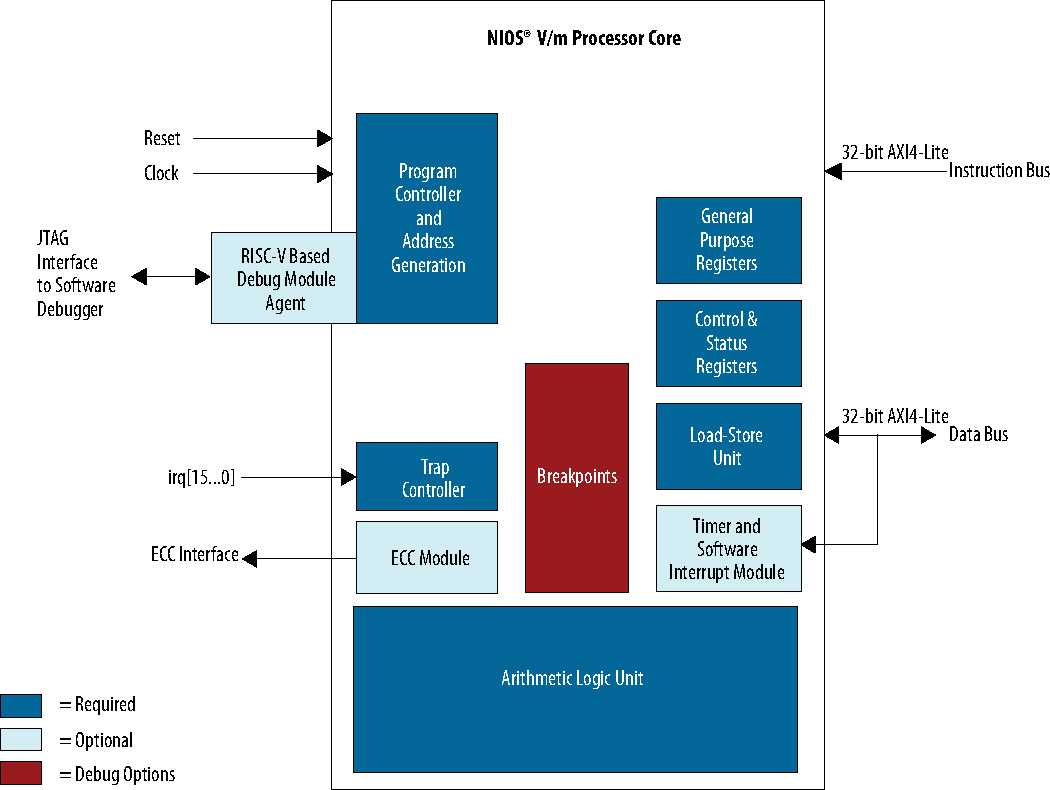
\includegraphics[width=0.6\linewidth]{Images/02_00_NiosVm_Architecture.pdf}
        \caption{Kiến trúc Nios V/m \cite{niosv_architecture}.}
        \label{fig:niosv_architecture}
    \end{figure}
    \item \textbf{Pipeline (Tùy chọn):} Nios V/m có thể được cấu hình với pipeline 5 tầng kinh điển (Fetch, Decode, Execute, Memory, Write back) để tăng hiệu suất hoặc không có pipeline (non-pipelined) để tối ưu diện tích. Khi sử dụng pipeline, có thể xảy ra hiện tượng stall (trì hoãn) do phụ thuộc dữ liệu (data dependency) hoặc tranh chấp tài nguyên (resource stall).
\end{itemize}

\section{Truy cập Bộ nhớ Trực tiếp (DMA)}
\acrfull{dma} là một tính năng của hệ thống máy tính cho phép một số hệ thống con phần cứng nhất định truy cập bộ nhớ hệ thống chính (\acrshort{ram}) để đọc và/hoặc ghi một cách độc lập với bộ xử lý trung tâm (CPU).
\begin{itemize}
    \item \textbf{Mục đích:} Giảm tải cho CPU trong các tác vụ truyền dữ liệu khối lượng lớn giữa bộ nhớ và các thiết bị ngoại vi (hoặc giữa các vùng nhớ khác nhau). Khi CPU khởi tạo một hoạt động DMA, nó có thể thực hiện các công việc khác trong khi bộ điều khiển DMA (DMA Controller - DMAC) thực hiện việc truyền dữ liệu.
    \item \textbf{Hoạt động:} CPU cấu hình DMAC với địa chỉ nguồn, địa chỉ đích, và số lượng dữ liệu cần truyền. Sau đó, CPU ra lệnh cho DMAC bắt đầu. DMAC chiếm quyền điều khiển bus hệ thống (hoặc sử dụng một bus riêng) để thực hiện việc truyền dữ liệu trực tiếp. Khi hoàn tất, DMAC thường thông báo cho CPU thông qua một ngắt (interrupt) hoặc bằng cách đặt một cờ trạng thái.
    \item \textbf{Lợi ích:} Tăng thông lượng dữ liệu, giải phóng CPU cho các tác vụ tính toán khác, cải thiện hiệu suất hệ thống tổng thể, đặc biệt quan trọng trong các hệ thống xử lý dữ liệu lớn hoặc thời gian thực.
\end{itemize}

% --- Section 4: Avalon Bus (Đã di chuyển từ Section 6 cũ) ---
\section{Giao tiếp Hệ thống: Bus Avalon}
\label{sec:avalon_bus}
Trong các hệ thống SoC được thiết kế trên nền tảng FPGA của Intel bằng công cụ Platform Designer, Giao tiếp Bus Avalon đóng vai trò là chuẩn kết nối (interconnect) nền tảng. 

Đặc tả Avalon bao gồm nhiều loại giao diện con, trong đó Avalon Memory-Mapped (Avalon-MM) là giao diện được sử dụng chủ yếu trong thiết kế bộ điều khiển DMA này để truy cập bộ nhớ và thanh ghi điều khiển.

\subsection{Giao tiếp Bus Avalon Memory Mapped Interface (Avalon-MM)}
Avalon-MM là một giao diện dựa trên địa chỉ, được thiết kế theo kiến trúc Master-Slave cho các giao dịch truy cập vào không gian bộ nhớ hoặc thanh ghi.

% Figure 02_01 (Existing)
\begin{figure}[htbp]
    \centering
    % Assumes this PDF is in the Images folder
    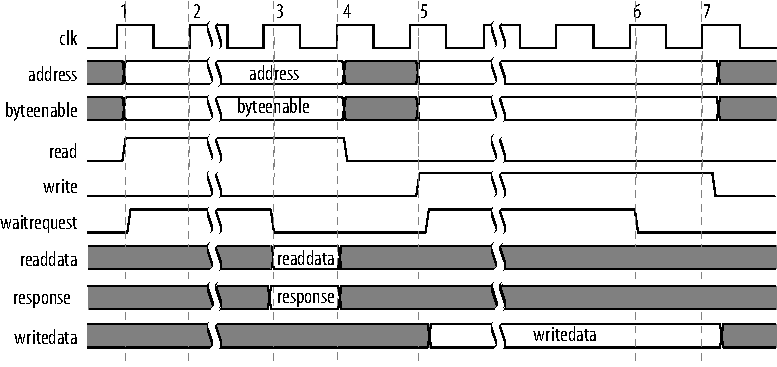
\includegraphics[width=\linewidth]{Images/02_01_Avalon_MM_Transfers.pdf}
    \caption{Các giao dịch đọc và ghi Avalon-MM điển hình với tín hiệu waitrequest \cite{avalon_mm_transfer}.}
    \label{fig:02_01_avalon_mm_transfer} % Kept original label
\end{figure}

\subsubsection{Đặc tả và Yêu cầu Giao thức}
\begin{itemize}
    \item \textbf{Vai trò Master/Slave:} 
    \begin{itemize}
        \item Một giao dịch luôn được khởi tạo bởi Master (ví dụ: CPU, DMA Master) và được phản hồi bởi Slave (ví dụ: Bộ nhớ, Thanh ghi DMA).
        \item Master chịu trách nhiệm cung cấp địa chỉ và tín hiệu điều khiển (\texttt{read}, \texttt{write}, \texttt{byteenable}), trong khi Slave giải mã địa chỉ, phản hồi bằng dữ liệu (\texttt{readdata}) hoặc chấp nhận ghi dữ liệu (\texttt{writedata}), và có thể sử dụng tín hiệu điều khiển luồng (\texttt{waitrequest}, \texttt{readdatavalid}).
    \end{itemize} 
    \item \textbf{Giao dịch Đọc (Read Transaction):}
        \begin{itemize}
            \item Master kích hoạt tín hiệu \texttt{read=1} và đưa ra \texttt{address}.
            \item Slave, sau khi giải mã địa chỉ và sẵn sàng dữ liệu, sẽ đặt dữ liệu lên \texttt{readdata}.
            \item \textbf{Điều khiển luồng (\texttt{waitrequest}):} Nếu Slave cần thêm thời gian (ví dụ: bộ nhớ chậm), nó sẽ kích hoạt \texttt{waitrequest=1}. Master \textit{phải} giữ nguyên \texttt{address} và \texttt{read} cho đến khi \texttt{waitrequest} bị hủy kích hoạt (\texttt{=0}). Slave trả về \texttt{readdata} trong chu kỳ clock mà \texttt{read=1} và \texttt{waitrequest=0}.
            \item \textbf{Tính hợp lệ dữ liệu (\texttt{readdatavalid}):} Trong các giao dịch đọc có độ trễ thay đổi (variable-latency reads, thường là pipelined), Slave sẽ kích hoạt \texttt{readdatavalid=1} cùng lúc với \texttt{readdata} để báo hiệu dữ liệu hợp lệ. Master \textit{phải} chỉ lấy dữ liệu khi \texttt{readdatavalid=1} (và \texttt{waitrequest=0}). Giao diện Read Master của DMA này (\texttt{READ\_MASTER}) được thiết kế để hỗ trợ \texttt{readdatavalid}.
            \item Giản đồ sóng đọc điển hình được minh họa trong Hình \ref{fig:02_01_avalon_mm_transfer} (phần Read), Hình \ref{fig:avalon_slave_waveforms}(a), \ref{fig:02_05_avalon_master_read}, và \ref{fig:memory_waveforms}(a).
        \end{itemize}
    \item \textbf{Giao dịch Ghi (Write Transaction):}
        \begin{itemize}
            \item Master kích hoạt \texttt{write=1}, đưa ra \texttt{address}, \texttt{writedata}, và \texttt{byteenable} (nếu có).
            \item \textbf{Điều khiển luồng (\texttt{waitrequest}):} Nếu Slave cần thêm thời gian để chuẩn bị nhận dữ liệu, nó sẽ kích hoạt \texttt{waitrequest=1}. Master *phải* giữ nguyên tất cả tín hiệu (\texttt{address}, \texttt{write}, \texttt{writedata}, \texttt{byteenable}) cho đến khi \texttt{waitrequest} bị hủy kích hoạt (\texttt{=0}). Slave sẽ ghi dữ liệu vào chu kỳ clock mà \texttt{write=1} và \texttt{waitrequest=0}.
            \item Tín hiệu \texttt{byteenable} cho phép ghi vào các byte cụ thể trong word dữ liệu (ví dụ: \texttt{4'b0011} chỉ ghi 2 byte thấp). Thiết kế DMA này sử dụng \texttt{byteenable=4'b1111} để ghi toàn bộ word 32-bit (Hình \ref{fig:02_02_memory_byteenable}).
            \item Giản đồ sóng ghi điển hình được minh họa trong Hình \ref{fig:02_01_avalon_mm_transfer} (phần Write), Hình \ref{fig:avalon_slave_waveforms}(b), \ref{fig:02_06_avalon_master_write}, và \ref{fig:memory_waveforms}(b).
        \end{itemize}
\end{itemize}

% Figure 02_02 (Existing, fixed label)
\begin{figure}[htbp]
    \centering
    % Assumes this PDF is in the Images folder
    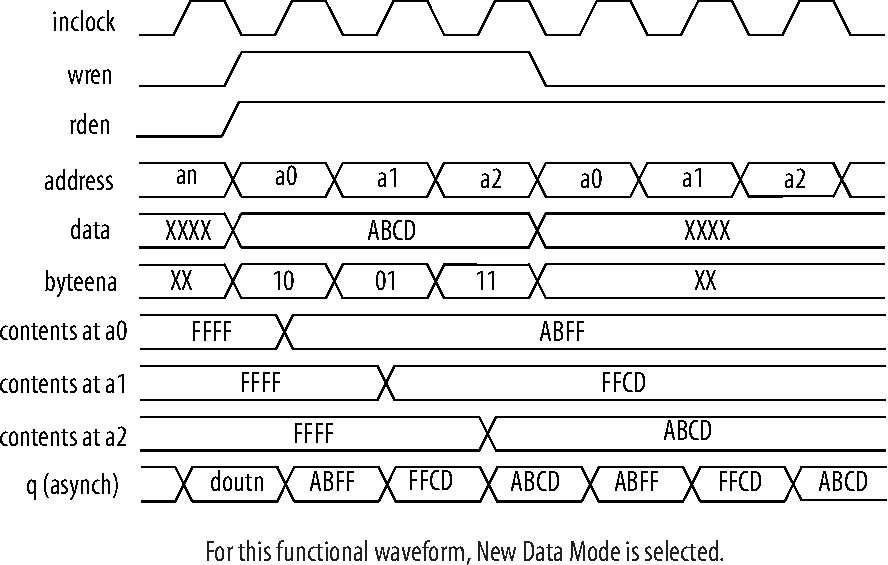
\includegraphics[width=\linewidth]{Images/02_02_Memory_ByteEnable.pdf}
    \caption{Giản đồ sóng chức năng của Byte Enable. Hình này minh họa ảnh hưởng của byte enable lên dữ liệu được ghi vào và đọc ra từ bộ nhớ \cite{memory_byteenable}.}
    \label{fig:02_02_memory_byteenable} % Fixed duplicate label
\end{figure}

Việc hiểu rõ và tuân thủ các yêu cầu về thời gian và hành vi của các tín hiệu này là cực kỳ quan trọng khi thiết kế một thành phần IP tương thích Avalon-MM.

% --- Section 5: Thiết kế và Kiến trúc DMA (Gộp từ Section 4, 5 cũ) ---
\section{Thiết kế và Kiến trúc Bộ điều khiển DMA Tùy chỉnh}
\label{sec:dma_design_and_architecture} % Label mới cho section gộp
Mục tiêu chính của việc thiết kế bộ điều khiển DMA này là tạo ra một thành phần phần cứng có khả năng truyền dữ liệu hiệu quả giữa các vùng nhớ trong hệ thống SoC trên FPGA, qua đó giảm tải cho bộ xử lý trung tâm Nios V/m. Để đạt được mục tiêu này, việc thiết kế phải tuân thủ các đặc tả giao tiếp của hệ thống bus Avalon-MM đã được trình bày ở Mục \ref{sec:avalon_bus}, đồng thời đảm bảo tính đúng đắn và hiệu quả của quá trình truyền dữ liệu.

Dựa trên yêu cầu về khả năng truyền dữ liệu tốc độ cao và độc lập với CPU, cũng như đặc tả của bus Avalon-MM, bộ điều khiển DMA tùy chỉnh được thiết kế với kiến trúc và các lựa chọn sau:

\subsection{Mục tiêu và Bối cảnh: Truyền dữ liệu giữa Bộ nhớ On-Chip}
\label{subsec:dma_context_onchip}
Một trong những ứng dụng ban đầu và quan trọng thúc đẩy việc thiết kế bộ điều khiển DMA này là nhu cầu truyền dữ liệu nhanh chóng và hiệu quả giữa các khối bộ nhớ trong chip (On-chip Memory - OCM) trên FPGA. Bộ nhớ on-chip, thường được hiện thực hóa bằng các khối RAM tích hợp sẵn trong cấu trúc FPGA, cung cấp tốc độ truy cập rất cao so với bộ nhớ ngoài (off-chip). Việc sử dụng DMA để di chuyển dữ liệu giữa các khối OCM (ví dụ: từ một vùng RAM chứa dữ liệu thô sang một vùng RAM khác để xử lý) giúp giải phóng CPU Nios V/m khỏi các vòng lặp sao chép bộ nhớ (\texttt{memcpy}) tốn thời gian, cho phép CPU tập trung vào các nhiệm vụ tính toán hoặc điều khiển khác.

Do đó, các giao diện Avalon-MM Master của \texttt{READ\_MASTER} và \texttt{WRITE\_MASTER} được thiết kế với giả định ban đầu là tương tác với các Slave là bộ nhớ on-chip. Điều này có nghĩa là chúng được tối ưu cho các giao dịch truy cập bộ nhớ có độ trễ tương đối thấp và ổn định, như được minh họa trong các giản đồ sóng đọc/ghi bộ nhớ (Hình \ref{fig:memory_waveforms}). Mặc dù vậy, thiết kế vẫn tuân thủ đầy đủ đặc tả Avalon-MM, cho phép DMA hoạt động với các loại bộ nhớ hoặc ngoại vi khác có hành vi thời gian khác nhau, miễn là chúng cũng tuân thủ chuẩn Avalon-MM.

\subsection{Kiến trúc Tổng thể và Luồng Dữ liệu}
Kiến trúc DMA được chọn dựa trên mô hình tách biệt luồng đọc và ghi dữ liệu để tối đa hóa thông lượng, bao gồm các khối chính sau:
\begin{itemize}
    \item \textbf{CONTROL\_SLAVE (`CONTROL\_SLAVE.v`):} Hoạt động như giao diện điều khiển Avalon-MM Slave cho CPU.
    \item \textbf{READ\_MASTER (`READ\_MASTER.v`):} Hoạt động như Avalon-MM Master để đọc dữ liệu từ bộ nhớ nguồn.
    \item \textbf{WRITE\_MASTER (`WRITE\_MASTER.v`):} Hoạt động như Avalon-MM Master để ghi dữ liệu vào bộ nhớ đích.
    \item \textbf{FIFO (`FIFO\_IP.v`):} Bộ đệm dữ liệu giữa Read và Write Master, được tạo từ IP Catalog của Quartus.
\end{itemize}
Luồng dữ liệu cơ bản diễn ra như sau: CPU cấu hình DMA thông qua \texttt{CONTROL\_SLAVE} (ghi địa chỉ nguồn, đích, độ dài). CPU kích hoạt DMA bằng cách ghi vào thanh ghi điều khiển. Khi được kích hoạt (\texttt{Start=1}), \texttt{READ\_MASTER} bắt đầu đọc dữ liệu từ bộ nhớ nguồn theo địa chỉ và độ dài đã cấu hình, đẩy dữ liệu vào FIFO. Đồng thời, \texttt{WRITE\_MASTER} đọc dữ liệu từ FIFO (khi FIFO không rỗng - \texttt{FF\_empty=0}) và ghi vào bộ nhớ đích theo cấu hình. \texttt{WRITE\_MASTER} báo hiệu hoàn thành (\texttt{WM\_done=1}) khi ghi xong từ cuối cùng, tín hiệu này được \texttt{CONTROL\_SLAVE} sử dụng để cập nhật thanh ghi trạng thái và tự động xóa bit Go.

\subsection{Thiết kế Module Điều khiển (`CONTROL\_SLAVE`)}
\begin{itemize}
    \item \textbf{Yêu cầu:} Cung cấp giao diện để CPU cấu hình (địa chỉ nguồn/đích, độ dài), khởi động và kiểm tra trạng thái DMA.
    \item \textbf{Giải pháp thiết kế (Dựa trên Avalon-MM Slave):}
        \begin{itemize}
            \item \textbf{Thanh ghi ánh xạ bộ nhớ:} Định nghĩa các thanh ghi nội bộ cho địa chỉ đọc (\texttt{readaddress\_reg}), địa chỉ ghi (\texttt{writeaddress\_reg}), độ dài (\texttt{length\_reg}), điều khiển (\texttt{control\_go}), và trạng thái (\texttt{status\_busy}, \texttt{status\_done}). Các thanh ghi này được gán các địa chỉ offset cụ thể (0, 1, 2, 4, 5) trong không gian địa chỉ 3-bit của module.
            \item \textbf{Logic giải mã địa chỉ:} Khi \texttt{iChipselect=1}, module giải mã \texttt{iAddress} từ CPU để xác định thanh ghi nào đang được truy cập cho thao tác đọc (\texttt{iRead=1}) hoặc ghi (\texttt{iWrite=1}).
            \item \textbf{Logic đọc/ghi:} Nếu đọc, dữ liệu từ thanh ghi được chọn sẽ được đưa ra \texttt{oReaddata}. Nếu ghi, dữ liệu từ \texttt{iWritedata} sẽ được ghi vào thanh ghi được chọn (ngoại trừ thanh ghi trạng thái chỉ có thể xóa bit Done).
            \item \textbf{Logic điều khiển/trạng thái:} Bit \texttt{GO} (bit 0 của thanh ghi điều khiển \texttt{iWritedata[0]} tại địa chỉ 4) được CPU ghi (\texttt{iWrite=1}) để khởi động DMA; giá trị này được chốt vào thanh ghi nội bộ \texttt{control\_go}. Tín hiệu \texttt{Start} được gán bằng \texttt{control\_go}. Module cập nhật \texttt{status\_busy} và \texttt{status\_done} dựa trên \texttt{Start} và tín hiệu \texttt{WM\_done} từ \texttt{WRITE\_MASTER}. Khi \texttt{WM\_done} tích cực, \texttt{status\_busy} bị xóa, \texttt{status\_done} được đặt, và quan trọng là \texttt{control\_go} cũng tự động bị xóa để ngăn DMA tự khởi động lại. Bit \texttt{status\_done} có thể được CPU xóa bằng cách ghi 1 vào bit 0 của thanh ghi trạng thái (địa chỉ 5).
        \end{itemize}
    \item \textbf{Mã nguồn tham khảo:} Phụ lục \ref{app:verilog_control_slave}.
\end{itemize}

\subsection{Thiết kế Module Master Đọc (\texttt{READ\_MASTER})}
\begin{itemize}
    \item \textbf{Yêu cầu:} Đọc tuần tự dữ liệu từ bộ nhớ nguồn theo cấu hình và đẩy vào FIFO, tuân thủ giao thức Avalon-MM Read Master và xử lý điều khiển luồng từ FIFO.
    \item \textbf{Giải pháp thiết kế (Dựa trên Avalon-MM Master và FSM):}
        \begin{itemize}
            \item \textbf{Giao diện Avalon-MM Master:} Module tạo tín hiệu \texttt{oRM\_read}, \texttt{oRM\_readaddress}. Nó phản hồi với \texttt{iRM\_waitrequest} bằng cách giữ nguyên trạng thái và tín hiệu yêu cầu đọc. Nó chỉ chấp nhận dữ liệu \texttt{iRM\_readdata} khi \texttt{iRM\_readdatavalid=1}.
            \item \textbf{Giao diện FIFO:} Module tạo tín hiệu \texttt{FF\_writerequest=1} và đưa \texttt{FF\_data} khi có dữ liệu hợp lệ từ Avalon bus và sẵn sàng ghi vào FIFO. Nó phản hồi với \texttt{FF\_almostfull} bằng cách tạm dừng gửi yêu cầu đọc Avalon mới để tránh làm đầy FIFO.
            \item \textbf{Máy trạng thái hữu hạn (FSM):} Quản lý chu trình đọc: Chờ \texttt{Start} (IDLE), kiểm tra FIFO không gần đầy (CHECK\_FIFO), gửi yêu cầu đọc Avalon (REQUEST), chờ \texttt{waitrequest=0} và sau đó là \texttt{readdatavalid=1} (WAIT\_DATA), ghi dữ liệu vào FIFO khi hợp lệ (WRITE\_FIFO), cập nhật địa chỉ/bộ đếm và quay lại kiểm tra FIFO/gửi yêu cầu mới (WAIT\_FIFO), lặp lại cho đến khi đọc đủ \texttt{Length} byte.
        \end{itemize}
    \item \textbf{Mã nguồn tham khảo:} Phụ lục \ref{app:verilog_read_master}.
\end{itemize}

\subsection{Thiết kế Module Master Ghi (\texttt{WRITE\_MASTER})}
\begin{itemize}
    \item \textbf{Yêu cầu:} Đọc dữ liệu từ FIFO (khi \texttt{FF\_empty=0}) và ghi tuần tự vào bộ nhớ đích theo cấu hình (\texttt{WM\_startaddress}, \texttt{Length}) khi \texttt{Start=1}, tuân thủ giao thức Avalon-MM Write Master (xử lý \texttt{iWM\_waitrequest}) và báo hiệu hoàn thành (\texttt{WM\_done=1}).
    \item \textbf{Giải pháp thiết kế (Dựa trên Avalon-MM Master và FSM):}
        \begin{itemize}
            \item \textbf{Giao diện FIFO:} Module kiểm tra \texttt{FF\_empty}. Nếu không rỗng, nó tạo tín hiệu \texttt{FF\_readrequest=1} để lấy dữ liệu \texttt{FF\_q} trong chu kỳ tiếp theo.
            \item \textbf{Giao diện Avalon-MM Master:} Module tạo tín hiệu \texttt{oWM\_write=1}, đưa ra địa chỉ ghi \texttt{oWM\_writeaddress}, dữ liệu ghi \texttt{oWM\_writedata} (lấy từ thanh ghi nội bộ chứa dữ liệu đọc từ FIFO), và \texttt{oWM\_byteenable=4'b1111}. Nó phản hồi với \texttt{iWM\_waitrequest=1} bằng cách giữ nguyên trạng thái và tất cả tín hiệu đầu ra Avalon.
            \item \textbf{Máy trạng thái hữu hạn (FSM):} Quản lý chu trình ghi: Chờ \texttt{Start} (IDLE), kiểm tra FIFO không rỗng (CHECK\_FIFO), yêu cầu đọc FIFO (READ\_FIFO), chờ dữ liệu FIFO được chốt (WAIT\_FIFO\_DATA), gửi yêu cầu ghi Avalon (START\_WRITE), chờ \texttt{waitrequest=0} (WAIT\_WRITE\_ACK), cập nhật địa chỉ/bộ đếm (UPDATE\_CNT). Lặp lại từ CHECK\_FIFO. Khi hoàn thành (\texttt{bytes\_remaining <= 4} trong trạng thái UPDATE\_CNT), FSM chuyển về IDLE và kích hoạt \texttt{WM\_done} trong một chu kỳ.
        \end{itemize}
    \item \textbf{Mã nguồn tham khảo:} Phụ lục \ref{app:verilog_write_master}.
\end{itemize}

\subsection{Tích hợp và Tín hiệu Giao tiếp}
Module \texttt{DMAController.v} (Phụ lục \ref{app:verilog_dmac}) đóng vai trò kết nối các module con (\texttt{CONTROL\_SLAVE}, \texttt{READ\_MASTER}, \texttt{WRITE\_MASTER}, \texttt{FIFO\_IP}) lại với nhau và cung cấp giao diện mức cao cho hệ thống. Bảng \ref{tab:dma_signals} liệt kê chi tiết các tín hiệu vào/ra của module này, thể hiện giao diện với CPU (qua Avalon Slave) và với bộ nhớ (qua Avalon Master).

\begin{figure}[htbp]
    \centering
    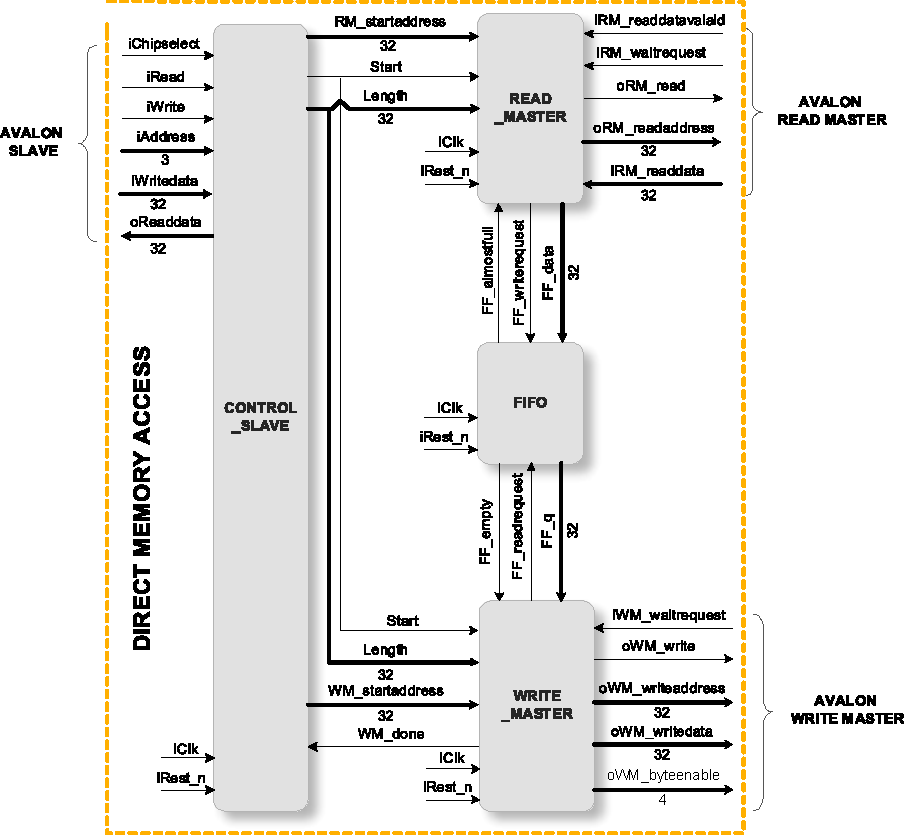
\includegraphics[width=\linewidth]{Images/02_09_DMABlockDiagram}
    \caption{Sơ đồ khối tổng thể của bộ điều khiển DMA.}
    \label{fig:02_09_DMA_BlockDiagram}
\end{figure}

\begin{figure}[htbp]
    \centering
    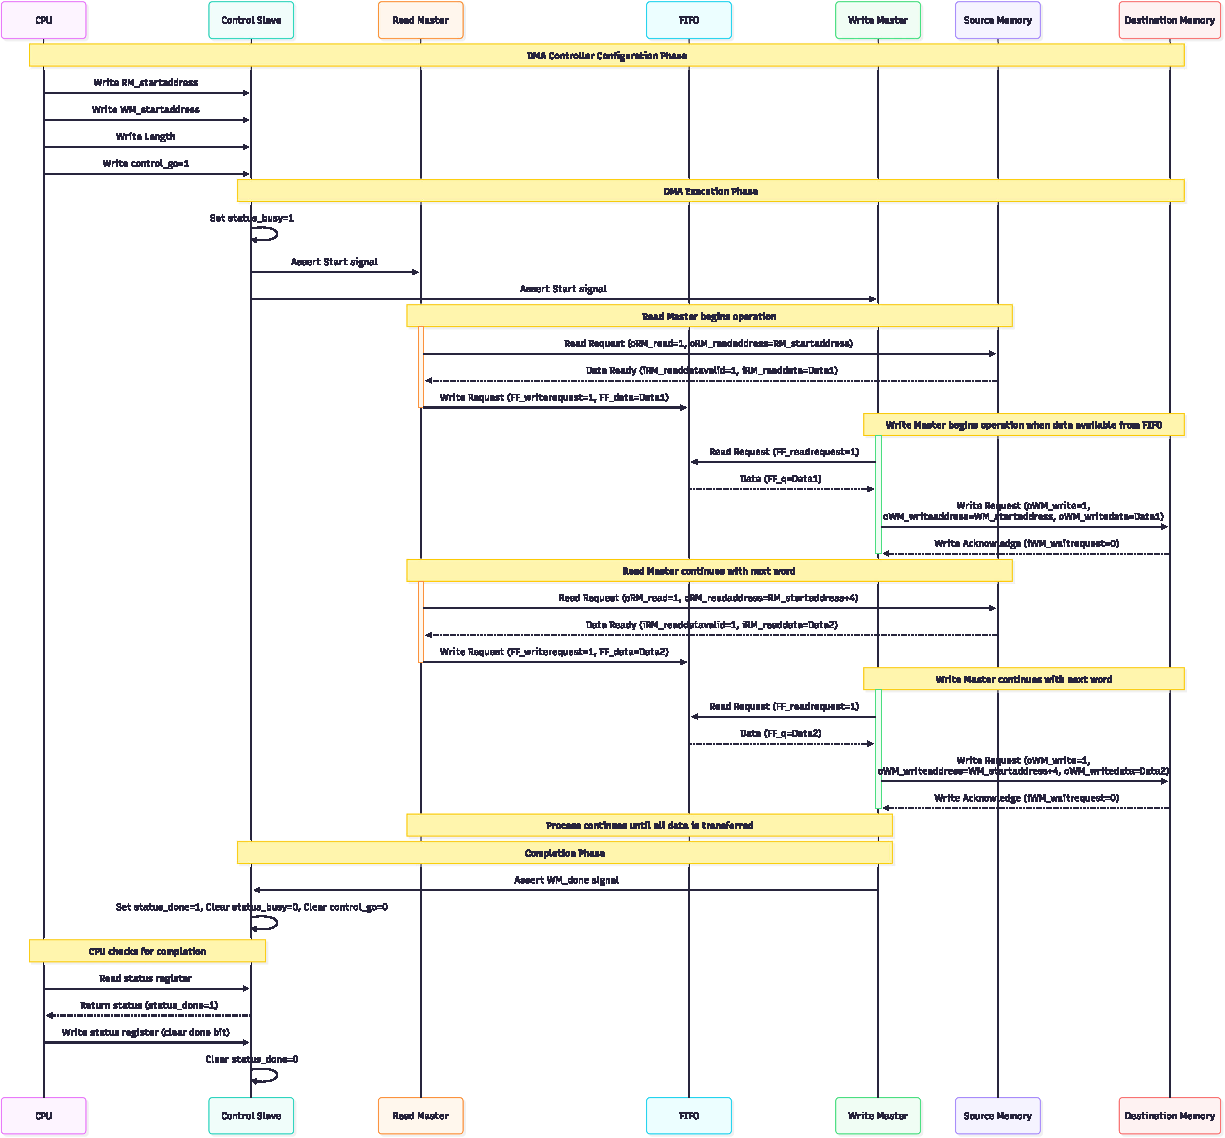
\includegraphics[width=\linewidth]{Images/02_10_SystemSequenceDiagram}
    \caption{Sơ đồ tuần tự hoạt động của DMA.}
    \label{fig:dma_flowchart_pdf}
\end{figure}

\begin{figure}[htbp]
    \centering
    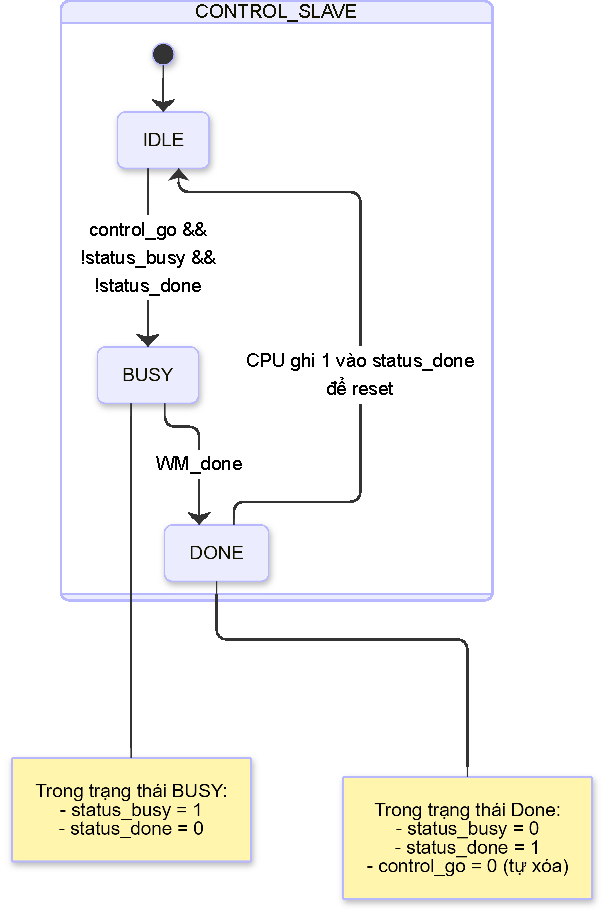
\includegraphics[width=0.5\linewidth]{Images/02_11_StateDiagram_ControlSlave}
    \caption{Sơ đồ trạng thái của module \texttt{CONTROL\_SLAVE}.}
    \label{fig:02_11_StateDiagram_ControlSlave}
\end{figure}

\begin{figure}[htbp]
    \centering
    % Subfigure for Memory Read
    \begin{subfigure}[b]{0.48\textwidth}
        \centering
        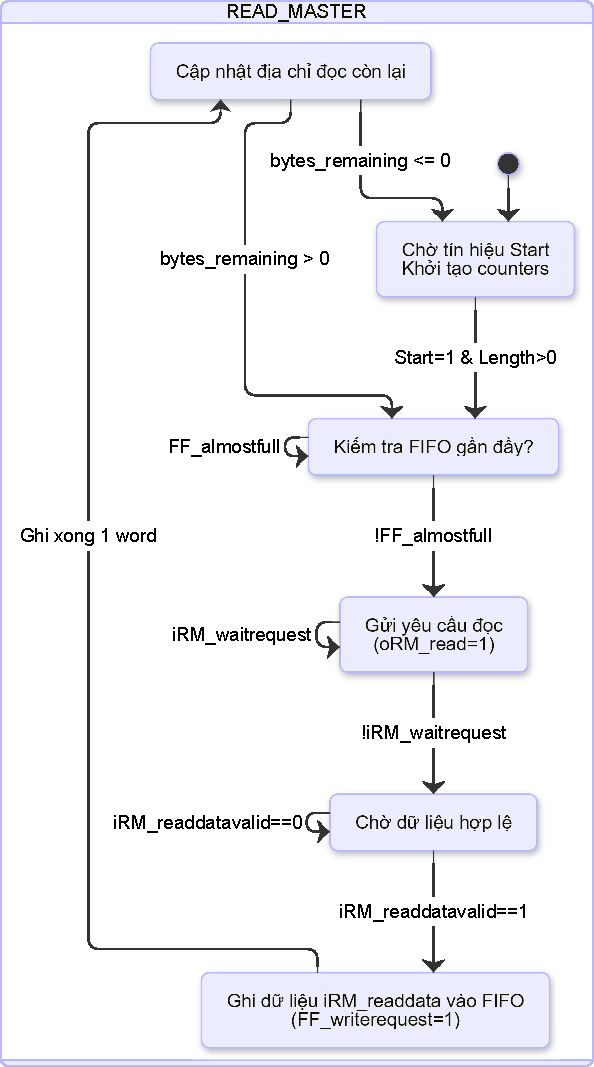
\includegraphics[width=\linewidth]{Images/02_12_StateDiagram_ReadMaster.pdf}
        \caption{\texttt{READ\_MASTER}.}
        \label{fig:02_12_StateDiagram_ReadMaster}
    \end{subfigure}
    \hfill % Thêm khoảng cách ngang
    % Subfigure for Memory Write
    \begin{subfigure}[b]{0.48\textwidth}
        \centering
        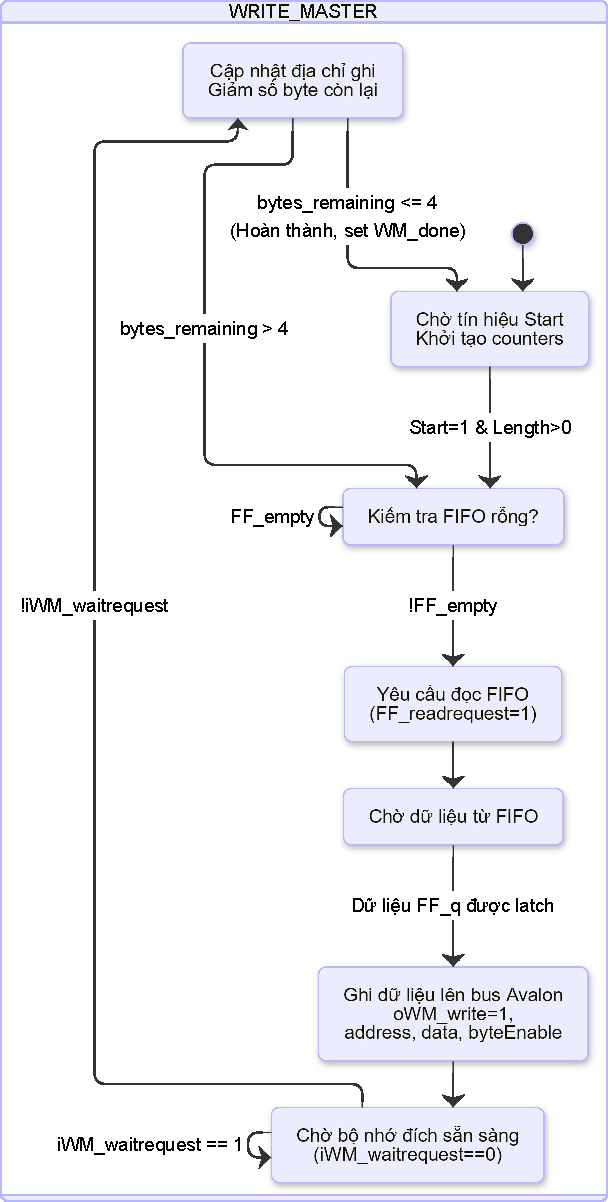
\includegraphics[width=\linewidth]{Images/02_13_StateDiagram_WriteMaster.pdf}
        \caption{\texttt{WRITE\_MASTER}.}
        \label{fig:02_13_StateDiagram_WriteMaster}
    \end{subfigure}
    \caption{Sơ đồ trạng thái các module.}
    \label{fig:memory_waveforms} % Nhãn chung cho cả cặp hình
\end{figure}

\subsection{Tín hiệu giao tiếp của DMA Controller} % Đã di chuyển bảng lên đây
Bảng \ref{tab:dma_signals} liệt kê các tín hiệu chính của module DMA Controller tùy chỉnh ở mức cao nhất (`DMAController.v`), thể hiện giao diện kết nối với CPU và hệ thống bus Avalon.

% --- Bảng tín hiệu DMA (Sử dụng định dạng gốc của người dùng) ---
\begin{table}[htbp]
    \centering
    \caption{Bảng mô tả tín hiệu chính của DMA Controller.}
    \label{tab:dma_signals}
    \begin{tabular}{@{}ccccp{7cm}@{}} % Định dạng gốc người dùng yêu cầu
        \toprule % Đường kẻ trên cùng
        \textbf{STT} & \textbf{Tên tín hiệu} & \textbf{Ngõ vào/ra} & \textbf{Số bit} & \textbf{Mô tả} \\
        \midrule % Đường kẻ giữa header và nội dung
        1 & \texttt{iClk} & In & 1 & Cấp xung clock 50 MHz cho DMA hoạt động \\
        2 & \texttt{iReset\_n} & In & 1 & \texttt{iReset\_n = 0}: reset lại DMA \\
        \midrule % Đường kẻ phân tách các nhóm tín hiệu
        \multicolumn{5}{@{}l}{\textbf{Giao tiếp Bus Avalon Slave (Từ CPU tới DMA)}} \\ % Sử dụng l căn trái cho tiêu đề nhóm
        \midrule
        3 & \texttt{iChipselect} & In & 1 & \texttt{iChipselect = 1}: cho phép truy xuất vào các thanh ghi trạng thái và điều khiển của DMA \\
        4 & \texttt{iRead} & In & 1 & \texttt{iRead = 1}: cho phép đọc giá trị của các thanh ghi trong DMA \\
        5 & \texttt{iWrite} & In & 1 & \texttt{iWrite = 1}: cho phép ghi giá trị vào các thanh ghi của DMA \\
        6 & \texttt{iAddress} & In & 3 & Chọn địa chỉ của thanh ghi cần đọc/ghi \\
        7 & \texttt{iWritedata} & In & 32 & Truyền giá trị cần ghi vào thanh ghi từ Avalon bus \\
        8 & \texttt{oReaddata} & Out & 32 & Xuất giá trị cần đọc từ thanh ghi ra Avalon bus \\
        \midrule
        \multicolumn{5}{@{}l}{\textbf{Giao tiếp Bus Avalon Read Master (Từ DMA tới Bộ nhớ Nguồn)}} \\
        \midrule
        9 & \texttt{iRM\_readdatavalid} & In & 1 & \texttt{=1}: báo hiệu \texttt{iRM\_readdata} hợp lệ \\
        10 & \texttt{iRM\_waitrequest} & In & 1 & \texttt{=1}: yêu cầu Read Master chờ \\
        11 & \texttt{oRM\_read} & Out & 1 & \texttt{=1}: yêu cầu đọc dữ liệu từ \texttt{oRM\_readaddress} \\
        12 & \texttt{oRM\_readaddress} & Out & 32 & Địa chỉ byte của vùng nhớ cần đọc \\
        13 & \texttt{iRM\_readdata} & In & 32 & Dữ liệu đọc được từ Avalon bus \\
        \midrule
        \multicolumn{5}{@{}l}{\textbf{Giao tiếp Bus Avalon Write Master (Từ DMA tới Bộ nhớ Đích)}} \\
        \midrule
        14 & \texttt{iWM\_waitrequest} & In & 1 & \texttt{=1}: yêu cầu Write Master chờ \\
        15 & \texttt{oWM\_write} & Out & 1 & \texttt{=1}: yêu cầu ghi dữ liệu vào \texttt{oWM\_writeaddress} \\
        16 & \texttt{oWM\_writeaddress} & Out & 32 & Địa chỉ byte của vùng nhớ cần ghi \\
        17 & \texttt{oWM\_writedata} & Out & 32 & Dữ liệu cần ghi ra Avalon bus \\
        18 & \texttt{oWM\_byteenable} & Out & 4 & Cho phép ghi từng byte (luôn là 4'b1111) \\
        \bottomrule
    \end{tabular}
\end{table}
% --- Kết thúc Bảng tín hiệu DMA ---

\FloatBarrier % Ngăn bảng và hình ảnh trôi qua section tiếp theo

\subsection{Hiện thực hóa Giao diện Avalon-MM trong DMA Controller}
Dựa trên đặc tả Avalon-MM, các giao diện của bộ điều khiển DMA tùy chỉnh được thiết kế như sau:
\begin{enumerate}
    \item \textbf{Giao diện Slave của \texttt{CONTROL\_SLAVE}:} Module này hoạt động như một Slave đơn giản, không sử dụng \texttt{waitrequest}. Nó giải mã \texttt{iAddress} khi \texttt{iChipselect=1} để đọc/ghi các thanh ghi nội bộ.
        \begin{itemize}
            \item \textbf{Khi đọc (\texttt{iRead=1}):} Dữ liệu từ thanh ghi tương ứng (địa chỉ nguồn/đích, độ dài, control, status) được đưa ra \texttt{oReaddata}. Hình \ref{fig:02_03_avalon_slave_read_sub}.
            \item \textbf{Khi ghi (\texttt{iWrite=1}):} Dữ liệu \texttt{iWritedata} được ghi vào thanh ghi cấu hình (địa chỉ nguồn/đích, độ dài) hoặc bit GO của thanh ghi điều khiển. Ghi 1 vào bit 0 của thanh ghi trạng thái sẽ xóa cờ Done. Hình \ref{fig:02_04_avalon_slave_write_sub}.
        \end{itemize}

    % Figures 02_03 and 02_04 side-by-side
    \begin{figure}[htbp]
        \centering
        \begin{subfigure}[b]{0.48\textwidth}
            \centering
            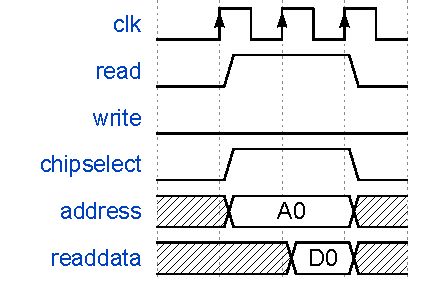
\includegraphics[width=\linewidth]{Images/02_03_AvalonSlave_ReadWaveform.pdf}
            \caption{Giản đồ sóng đọc Slave.}
            \label{fig:02_03_avalon_slave_read_sub}
        \end{subfigure}
        \hfill
        \begin{subfigure}[b]{0.48\textwidth}
            \centering
            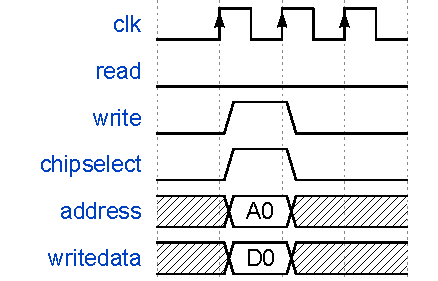
\includegraphics[width=\linewidth]{Images/02_04_AvalonSlave_WriteWaveform.pdf}
            \caption{Giản đồ sóng ghi Slave.}
            \label{fig:02_04_avalon_slave_write_sub}
        \end{subfigure}
        \caption{Giản đồ sóng đọc và ghi của giao tiếp Avalon-MM Slave.}
        \label{fig:avalon_slave_waveforms}
    \end{figure}

    \item \textbf{Giao diện Master của \texttt{READ\_MASTER}:} Module chủ động tạo giao dịch đọc, xử lý \texttt{waitrequest} và \texttt{readdatavalid}.
        \begin{itemize}
            \item Kích hoạt \texttt{oRM\_read=1} và đưa ra \texttt{oRM\_readaddress}.
            \item Nếu \texttt{iRM\_waitrequest=1}, giữ nguyên tín hiệu và trạng thái.
            \item Khi \texttt{iRM\_waitrequest=0}, chờ \texttt{iRM\_readdatavalid=1} mới lấy dữ liệu \texttt{iRM\_readdata} và ghi vào FIFO. Hình \ref{fig:02_05_avalon_master_read}.
        \end{itemize}

    \begin{figure}[htbp]
        \centering
        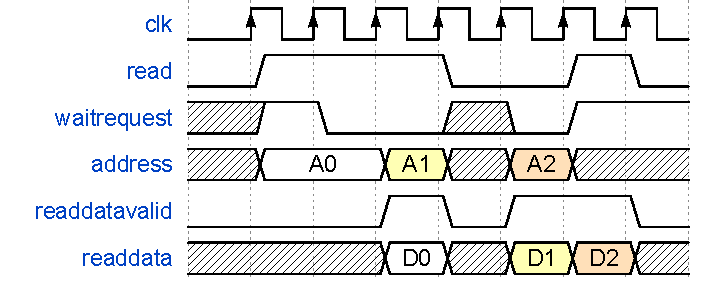
\includegraphics[width=\linewidth]{Images/02_05_AvalonMaster_ReadWaveform.pdf}
        \caption{Giản đồ sóng đọc của giao tiếp Avalon-MM Master.}
        \label{fig:02_05_avalon_master_read}
    \end{figure}

    \item \textbf{Giao diện Master của \texttt{WRITE\_MASTER}:} Module chủ động tạo giao dịch ghi, xử lý \texttt{waitrequest}.
        \begin{itemize}
            \item Kích hoạt \texttt{oWM\_write=1}, đưa ra \texttt{oWM\_writeaddress}, \texttt{oWM\_writedata}, và \texttt{oWM\_byteenable = 4'b1111}.
            \item Nếu \texttt{iWM\_waitrequest=1}, giữ nguyên tất cả tín hiệu đầu ra và trạng thái.
            \item Khi \texttt{iWM\_waitrequest=0}, giao dịch ghi được xem là hoàn thành, FSM chuyển trạng thái. Hình: \ref{fig:02_06_avalon_master_write}.
        \end{itemize}

    \begin{figure}[htbp]
        \centering
        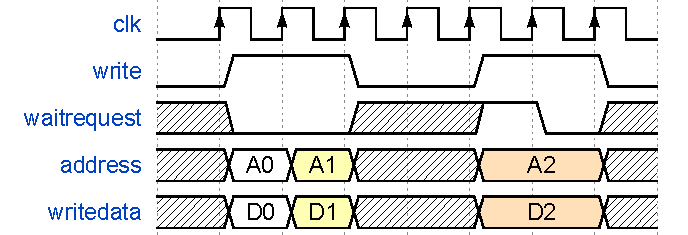
\includegraphics[width=\linewidth]{Images/02_06_AvalonMaster_WriteWaveform.pdf}
        \caption{Giản đồ sóng ghi của giao tiếp Avalon-MM Master.}
        \label{fig:02_06_avalon_master_write}
    \end{figure}
\end{enumerate}
Việc thiết kế các giao diện DMA dựa trên và tuân thủ chặt chẽ đặc tả Avalon-MM là yếu tố then chốt đảm bảo bộ điều khiển DMA tùy chỉnh có thể hoạt động chính xác và tích hợp liền mạch vào hệ thống SoC Nios V trên Platform Designer.

\begin{figure}[htbp]
    \centerin
    % Subfigure for Memory Read
    \begin{subfigure}[b]{0.48\textwidth}
        \centering
        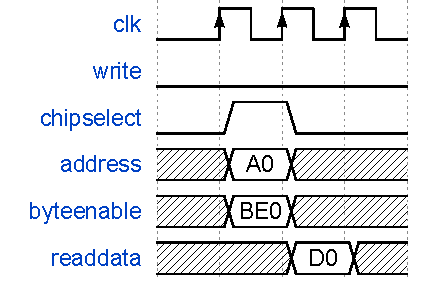
\includegraphics[width=\linewidth]{Images/02_07_Memory_ReadWaveform.pdf}
        \caption{Giản đồ sóng đọc Memory.}
        \label{fig:02_07_memory_read_sub}
    \end{subfigure}
    \hfill
    \begin{subfigure}[b]{0.48\textwidth}
        \centering
        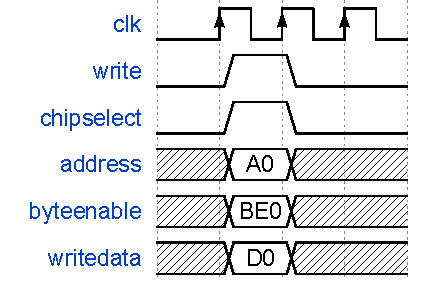
\includegraphics[width=\linewidth]{Images/02_08_Memory_WriteWaveform.pdf}
        \caption{Giản đồ sóng ghi Memory.}
        \label{fig:02_08_memory_write_sub}
    \end{subfigure}
    \caption{Giản đồ sóng đọc và ghi bộ nhớ qua giao tiếp Avalon-MM.}
    \label{fig:memory_waveforms}
\end{figure}


\section{TRIỂN KHAI VÀ KIỂM THỬ HỆ THỐNG NIOS V VỚI DMA}
\label{sec:chapter3_content} % Changed label from Chapter3
Phần \ref{sec:chapter3_content} trình bày chi tiết quy trình từng bước được thực hiện để triển khai và kiểm thử một Hệ thống trên Chip (\acrshort{soc}) dựa trên bộ xử lý mềm (soft-core processor) Nios V/m của Intel, tích hợp một bộ điều khiển Truy cập Bộ nhớ Trực tiếp (\acrfull{dma}) tùy chỉnh. Nền tảng phần cứng mục tiêu là bo mạch phát triển (development board) Terasic DE10-Standard \cite{terasicDE10Std} trang bị \acrshort{fpga} Intel Cyclone V \acrshort{soc}. Việc triển khai sử dụng Phần mềm Quartus Prime Lite Edition của Intel, Platform Designer (trước đây là Qsys), và \acrshort{ide} Ashling RiscFree™ \cite{ashling_riscfree_guide} cho việc phát triển và gỡ lỗi (debug) phần mềm.
\subsection{Xây dựng Hệ thống Phần cứng trên Quartus Prime}
\label{sec:build_hardware}

Phần này bao gồm việc tạo dự án Quartus và thiết kế hệ thống phần cứng bằng Platform Designer.

\begin{enumerate}
    \item \textbf{Tạo Dự án Quartus:}
    \begin{itemize}
        \item Khởi động Quartus Prime Lite Edition.
        \item Tạo một dự án mới bằng Trình hướng dẫn Dự án Mới (New Project Wizard) (File -> New Project Wizard...).
        \item Chỉ định thư mục làm việc (working directory) và tên dự án (project name) (ví dụ: \texttt{D:\textbackslash FETEL\_WorkDir\textbackslash Y4S2\_DMANiosVIntern}, \texttt{DMANiosV}) (Hình \ref{fig:03_11}).
        \item Chọn thiết bị mục tiêu (target device) tương ứng với bo mạch DE10-Standard: Họ (Family) `Cyclone V`, Thiết bị (Device) \texttt{5CSXFC6D6F31C6} (Hình \ref{fig:03_12}).
    \end{itemize}
    \item \textbf{Chuẩn bị các tệp Verilog DMA Controller:} Sao chép các tệp nguồn Verilog được cung cấp cho bộ điều khiển DMA (\texttt{DMAController.v} (\ref{app:verilog_dmac}), \texttt{CONTROL\_SLAVE.v} (\ref{app:verilog_control_slave}), \texttt{FIFO\_IP.v}, \texttt{READ\_MASTER.v} (\ref{app:verilog_read_master}), \texttt{WRITE\_MASTER.v} (\ref{app:verilog_write_master})) vào thư mục dự án Quartus (Hình \ref{fig:03_13}).
    \item \textbf{Tạo Hệ thống Platform Designer:}
    \begin{itemize}
        \item Khởi chạy Platform Designer (Tools -> Platform Designer).
        \item \textbf{Thêm Bộ xử lý Nios V/m:} Trong IP Catalog, tìm và thêm "Nios V/m Microcontroller Intel FPGA IP". Trong cấu hình của nó, bật tùy chọn  "Enable Reset from Debug Module" để dễ dàng reset phần mềm khi gỡ lỗi (Hình \ref{fig:03_15}).
        \item \textbf{Thêm Bộ nhớ Trên Chip (On-Chip Memory):} Thêm instances của IP "On-Chip Memory (\acrshort{ram} or \acrshort{rom})". Cấu hình cả hai là \acrshort{ram}. Đặt "Tổng dung lượng bộ nhớ (Total memory size)" cho mỗi bộ nhớ là 131072 byte (128 KB) (Cấu hình ví dụ Hình \ref{fig:03_16}). Một bộ nhớ (\texttt{onchip\_memory2\_0}) cho lệnh (instructions), và bộ nhớ còn lại (\texttt{onchip\_memory2\_1}) sẽ được sử dụng cho dữ liệu (data).
        \item \textbf{Thêm JTAG UART:} Thêm "\acrshort{jtag} \acrshort{uart} Intel FPGA IP" để giao tiếp (communication) giữa bộ xử lý Nios V và máy tính chủ (host PC) thông qua kết nối \acrshort{jtag} (cho việc in ra terminal \texttt{printf}).
        \item \textbf{Tạo IP DMA Controller:}
        \begin{itemize}
            \item Trong IP Catalog, chọn "New Component...".
            \item Trong Component Editor, đặt tên (ví dụ: \texttt{DMA\_Controller}).
            \item Chuyển đến tab "Files". Thêm tất cả các tệp Verilog DMA tùy chỉnh (`.v`). Đặt \texttt{DMAController.v} làm Top-Level File bằng cách nhấp đúp vào "Attributes". 
            \item Nhấp vào "Analyze Synthesis Files" để Quartus tổng hợp các tệp Verilog. Nhấn vào "Copy from Synthesis Files" để điền các tệp mô phỏng (simulation files) (Hình \ref{fig:03_21}).
            \item Chuyển đến tab "Signals". Sau đó cấu hình các tín hiệu như hình \ref{fig:03_23}. 
            \item Chuyển đến tab "Signals \& Interfaces". Đảm bảo các interface được cấu hình như sau (Hình \ref{fig:03_26}, \ref{fig:03_27}):
            \begin{itemize}
                \item Ngõ vào Đồng hồ (Clock input - \texttt{clk}): \texttt{clock\_sink}.
                \item Ngõ vào Reset (\texttt{reset\_n}): \texttt{reset\_sink}.
                \item Associated Clock: \texttt{clk} .
                \item Associated Reset: \texttt{reset\_n}.
            \end{itemize}
            \item Nhấp vào "Finish..." để lưu IP DMA Controller (tệp `.tcl`).
        \end{itemize}
        \item \textbf{Thêm IP DMA Controller vào Hệ thống \acrshort{soc}}.
        \item \textbf{Kết nối các Thành phần:} Thực hiện kết nối như hình \ref{fig:03_28}.
        \item \textbf{Gán Địa chỉ Cơ sở (Assign Base Addresses):} Đi đến menu "System" và chọn "Assign Base Addresses" (Hình \ref{fig:03_29}). Công cụ sẽ tự động gán các địa chỉ không trùng lặp cho tất cả các giao diện slave. Các địa chỉ này được lưu trong thư viện BSP dưới file \textbf{system.h}.
        \item \textbf{Thay Nios V (Vector Reset):} Vector reset (reset vector) của Nios V cần trỏ đến bộ nhớ chứa mã lệnh ban đầu (initial program code memory). 
        \begin{itemize}
            \item Ngắt kết nối \texttt{instruction\_master} khỏi \texttt{onchip\_memory2\_1} (hình \ref{fig:03_30}). 
            \item Mở lại cấu hình Nios V/m (nhấp đúp). Đặt "Bộ nhớ Vector Reset (Reset Agent)" thành \texttt{onchip\_memory2\_0.s1} (hình \ref{fig:03_31}).
        \end{itemize}
        \item \textbf{Lưu Hệ thống:} Lưu hệ thống Platform Designer (\texttt{system.qsys}).
    \end{itemize}
    \item \textbf{Generate HDL:} Trong Platform Designer, nhấp vào nút "Generate HDL..." và nhấp vào "Generate" (Hình \ref{fig:03_34}). Thao tác này tạo ra các tệp Verilog đại diện cho hệ thống \acrshort{soc} được kết nối với nhau. Sau khi tổng hợp thành công, ta tích hợp hệ thống vào thiết kế bằng việc thêm tệp `.qip` vào Project Quartus.
    \item \textbf{Tích hợp Hệ thống vào Project Quartus:}
    \begin{itemize}
        \item Trong Quartus, thêm tệp `.qip` được tạo (\texttt{system/synthesis/system.qip}) vào project (Project -> Add/Remove Files in Project...) (Hình \ref{fig:03_37}, Hình \ref{fig:03_38}).
        \item Tạo một tệp Verilog top-level (\texttt{DMANiosV.v} \ref{lst:verilog_top}) để khởi tạo hệ thống được tạo ra, kết nối các ngõ vào đồng hồ (clock) và reset của hệ thống tương ứng với ngõ vào đồng hồ của \acrshort{fpga} (\texttt{CLOCK\_50}) và một nút reset (\texttt{KEY[0]}) (Hình \ref{fig:03_42}). 
    \end{itemize}
    \item \textbf{Import cấu hình chân (Import Pin Assignments):} Sử dụng tệp gán chân DE10-Standard (`.qsf`) được cung cấp từ FPGAcademy \cite{fpgacademy-qsf}, \cite{fpgacademy-boards}. Trong Quartus, mở menu Assignments -> Import Assignments... (Hình \ref{fig:03_39}). Duyệt đến tệp `.qsf` đã tải xuống và import nó (Hình \ref{fig:03_40}).
    \item \textbf{Biên dịch thiết kế (Compile Design):} Chạy quy trình biên dịch toàn bộ trong Quartus (Processing -> Start Compilation) (Hình \ref{fig:03_41}). Xác minh biên dịch thành công và kiểm tra các gán chân trong Assignment Editor (Assignments -> Assignment Editor) (Hình \ref{fig:03_42}). Thao tác này tạo ra tệp `.sof` cần thiết để lập trình \acrshort{fpga}.
\end{enumerate}

% Figure environments for Section 3.2
\begin{figure}[htbp] \centering 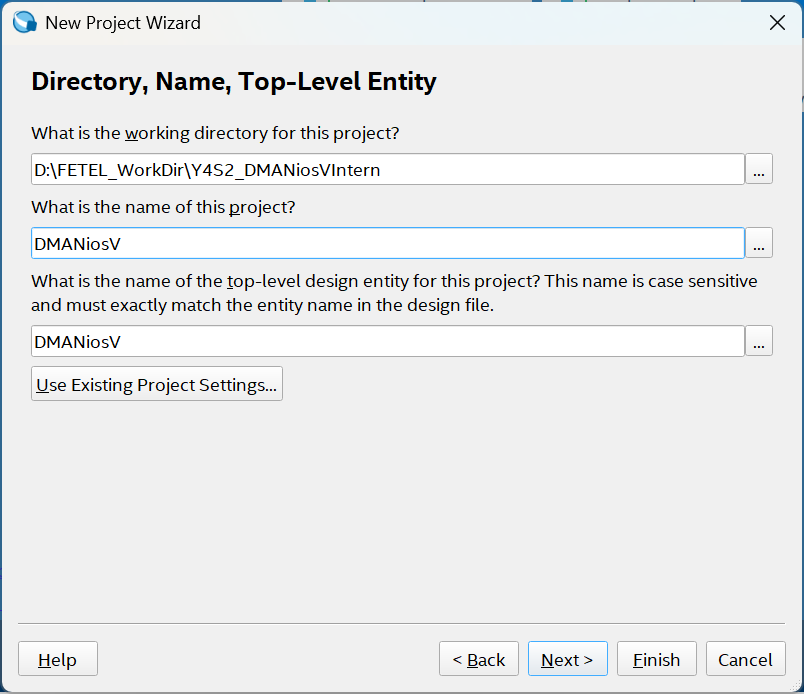
\includegraphics[width=0.7\linewidth]{03_11_QuartusNewProjectWizard1.png} \caption{Quartus: New Project Wizard: Chỉ định đường dẫn thư mục và tên Project.} \label{fig:03_11} \end{figure}
\begin{figure}[htbp] \centering 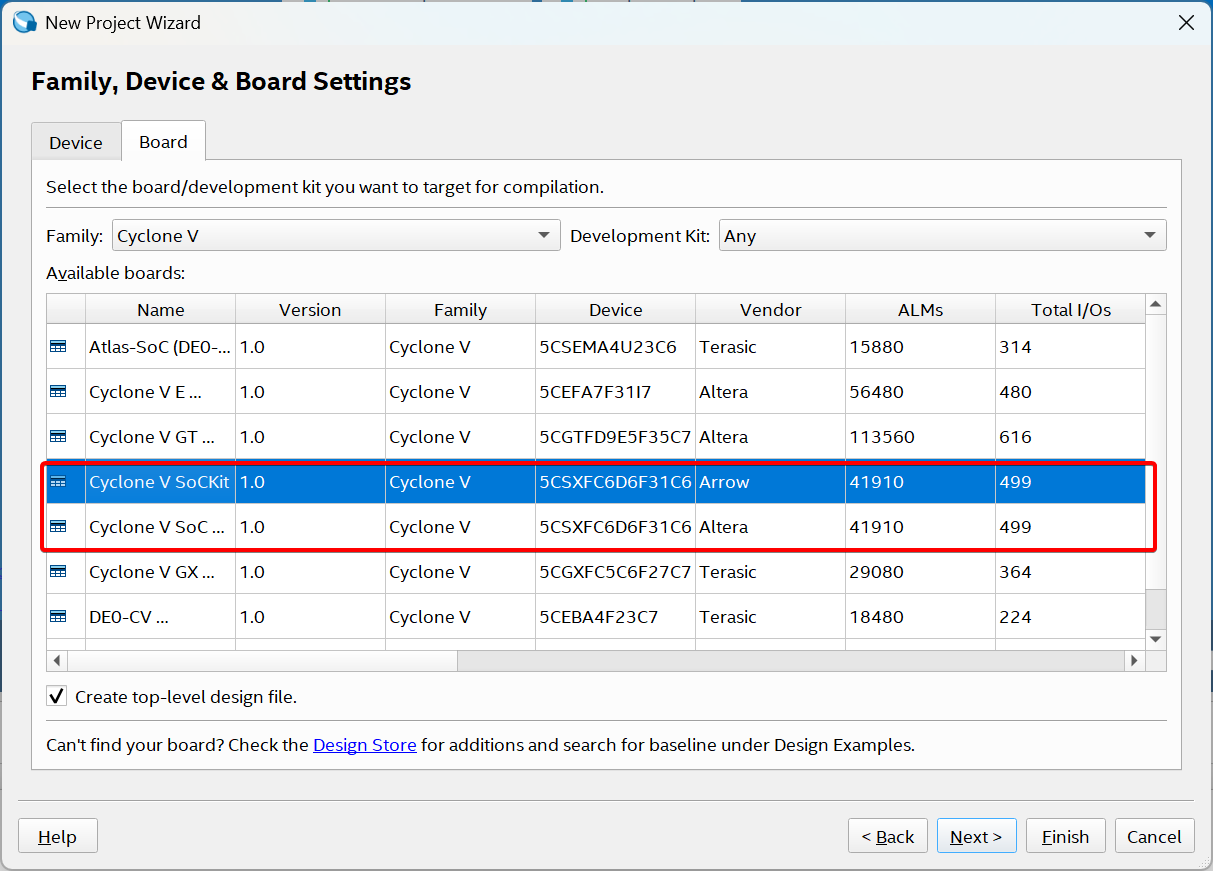
\includegraphics[width=0.9\linewidth]{03_12_QuartusNewProjectWizard2.png} \caption{Quartus: New Project Wizard: Device Selector} \label{fig:03_12} \end{figure}
\begin{figure}[htbp] \centering 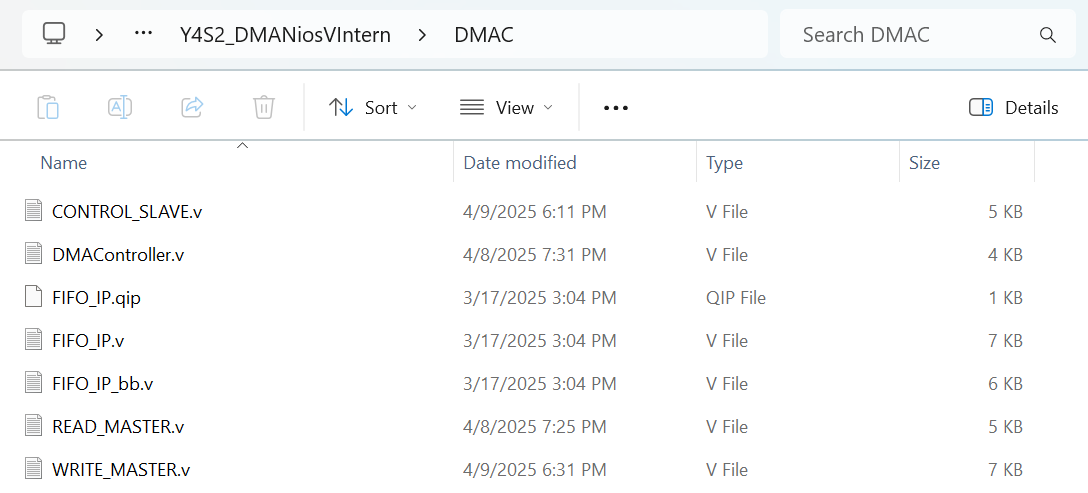
\includegraphics[width=0.9\linewidth]{03_13_ProjectFilesDMA.png} \caption{Thư mục dự án hiển thị các tệp Verilog DMA tùy chỉnh đã sao chép.} \label{fig:03_13} \end{figure}
% \begin{figure}[htbp] \centering 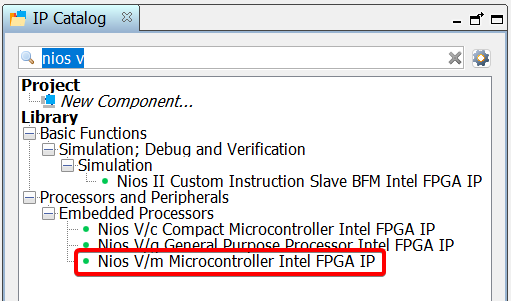
\includegraphics[width=0.6\linewidth]{03_14_IPCatalogNiosVSelection.png} \caption{Platform Designer IP Catalog: Chọn Nios V/m Microcontroller.} \label{fig:03_14} \end{figure}
\begin{figure}[htbp] \centering 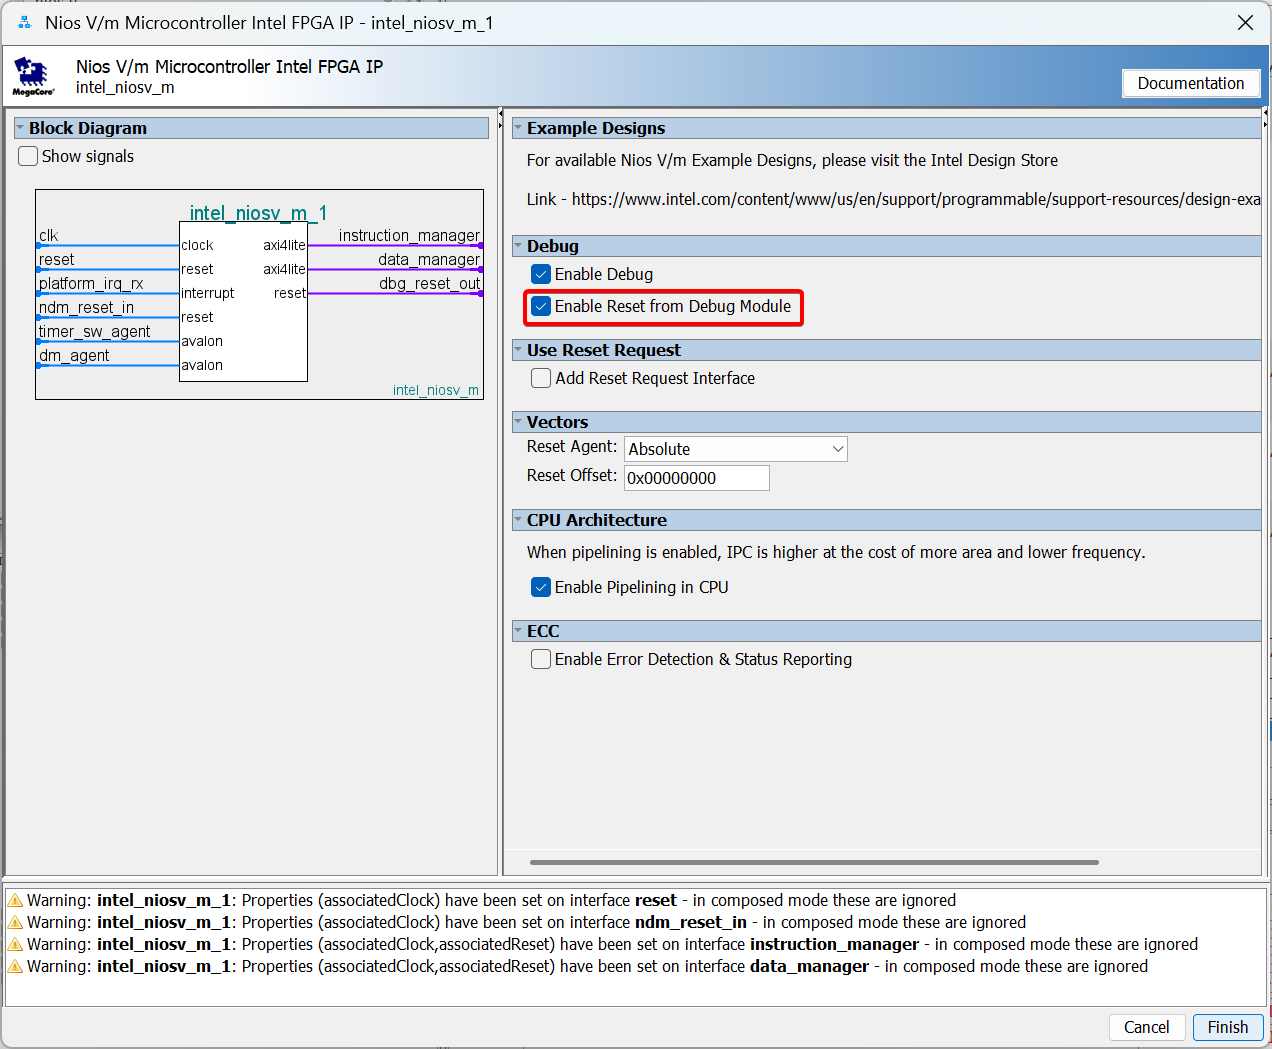
\includegraphics[width=0.9\linewidth]{03_15_NiosVIPConfig1.png} \caption{Cấu hình IP Nios V/m: Bật "Enable Reset from Debug Module".} \label{fig:03_15} \end{figure}
\begin{figure}[htbp] \centering 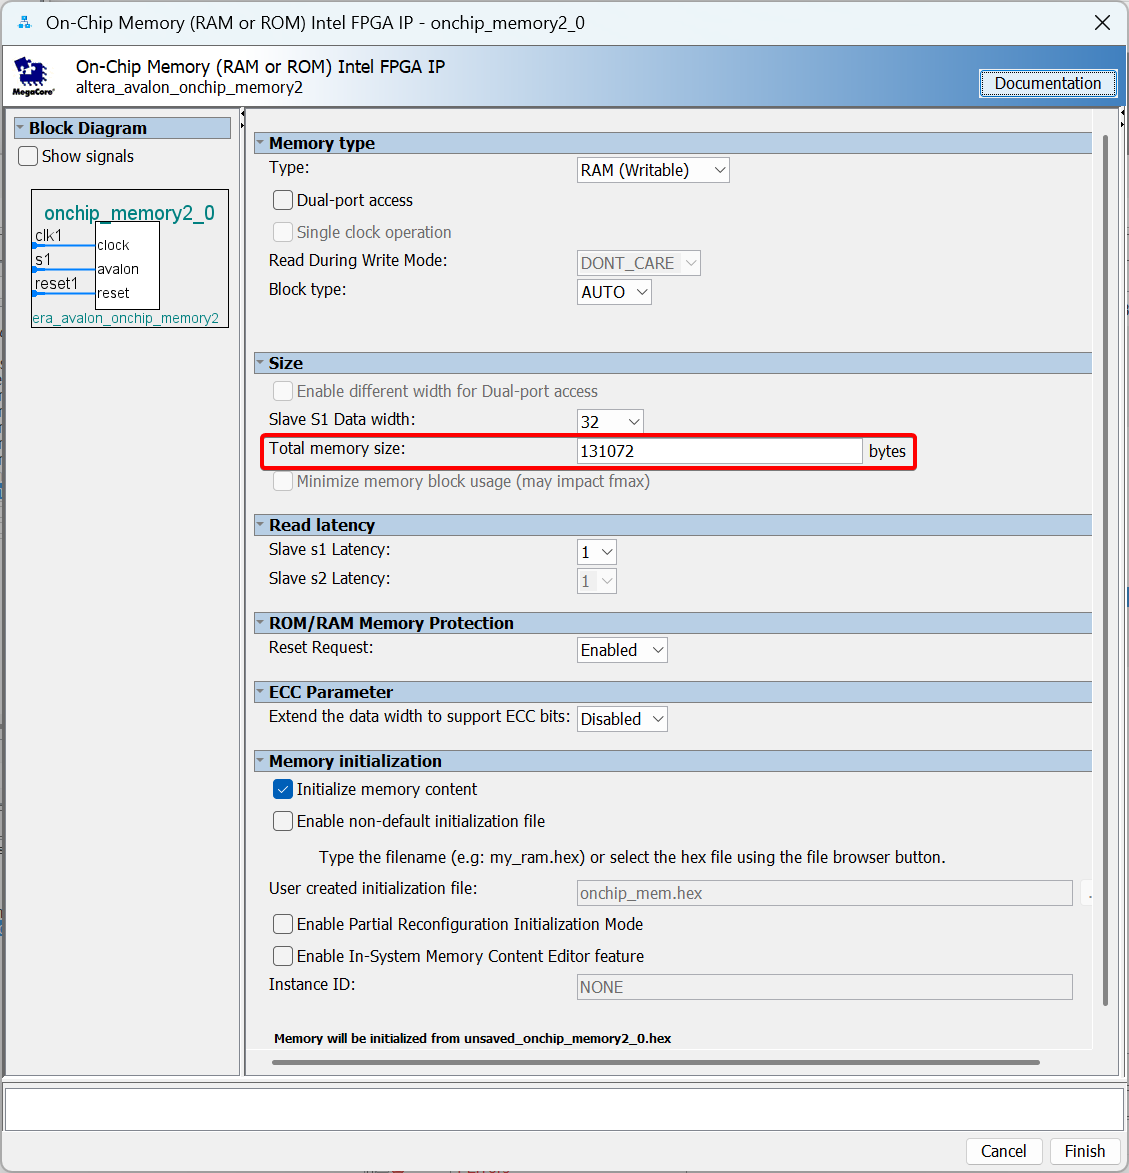
\includegraphics[width=0.9\linewidth]{03_16_OnChipMemoryIPConfig.png} \caption{Cấu hình IP Bộ nhớ Trên Chip: Đặt kích thước thành 128 KB.} \label{fig:03_16} \end{figure}
\begin{figure}[htbp] \centering 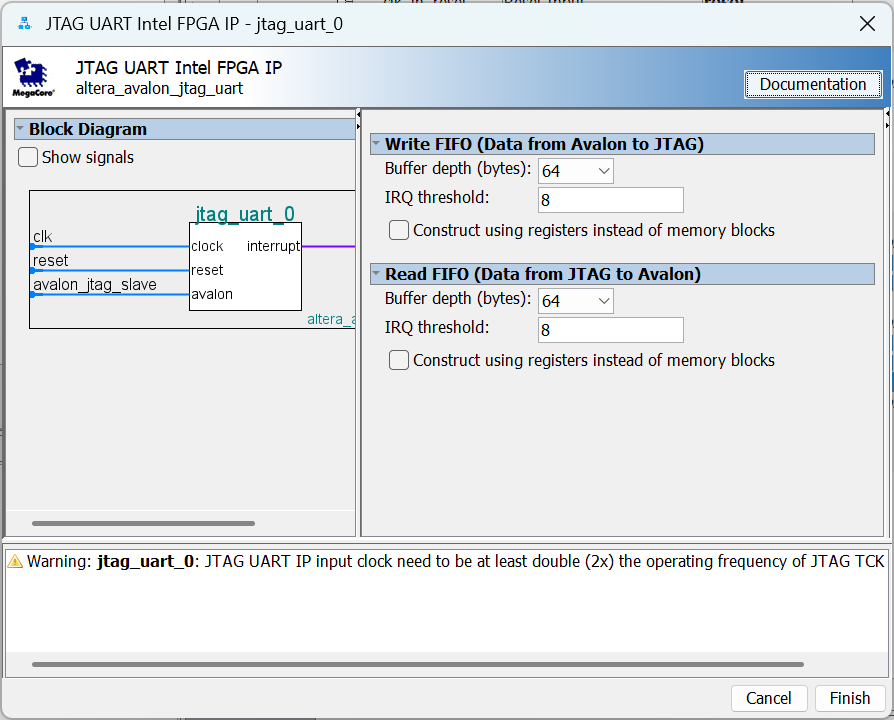
\includegraphics[width=0.9\linewidth]{03_17_JTAGUARTIPConfig.png} \caption{Cấu hình IP JTAG UART.} \label{fig:03_17} \end{figure}
% \begin{figure}[htbp] \centering 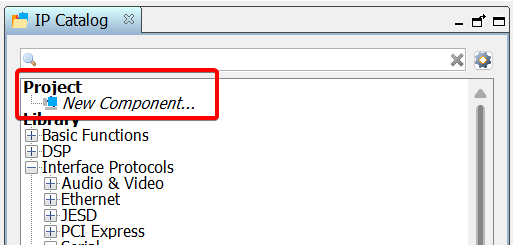
\includegraphics[width=0.6\linewidth]{03_18_IPCatalog_AddComponent.png} \caption{IP Catalog Platform Designer: Chọn "New Component...".} \label{fig:03_18} \end{figure}
% \begin{figure}[htbp] \centering 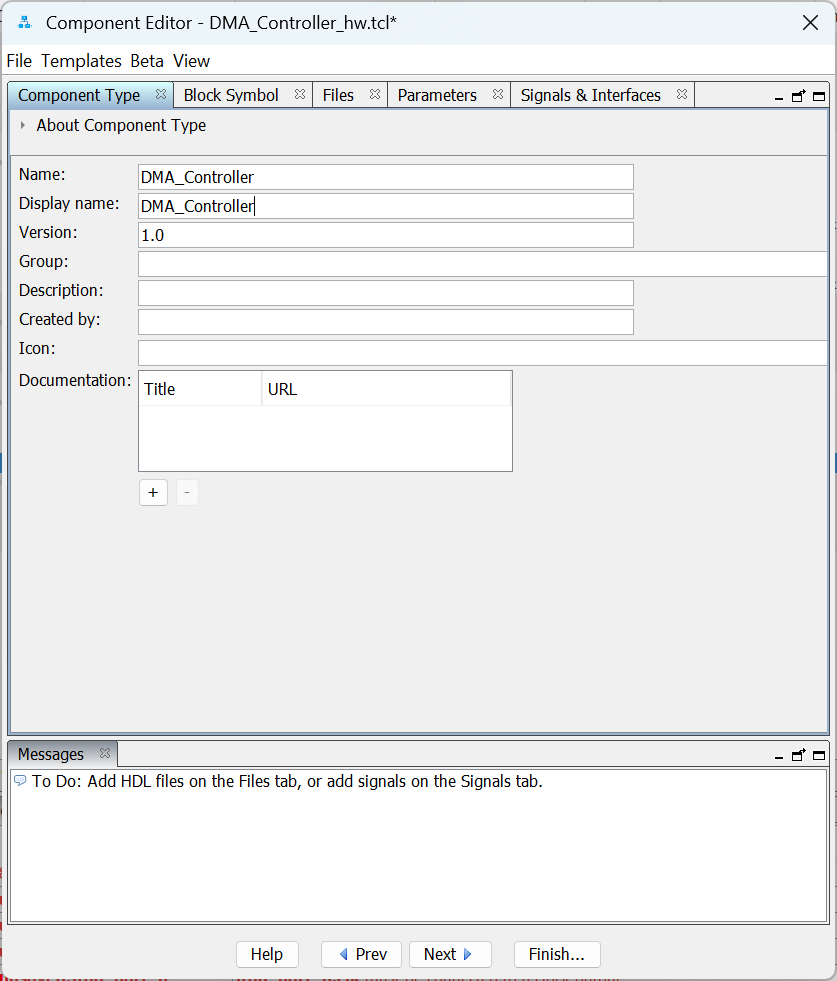
\includegraphics[width=0.9\linewidth]{03_19_ComponentEditorType.png} \caption{Component Editor: Đặt tên cho thành phần DMA tùy chỉnh.} \label{fig:03_19} \end{figure}
% \begin{figure}[htbp] \centering 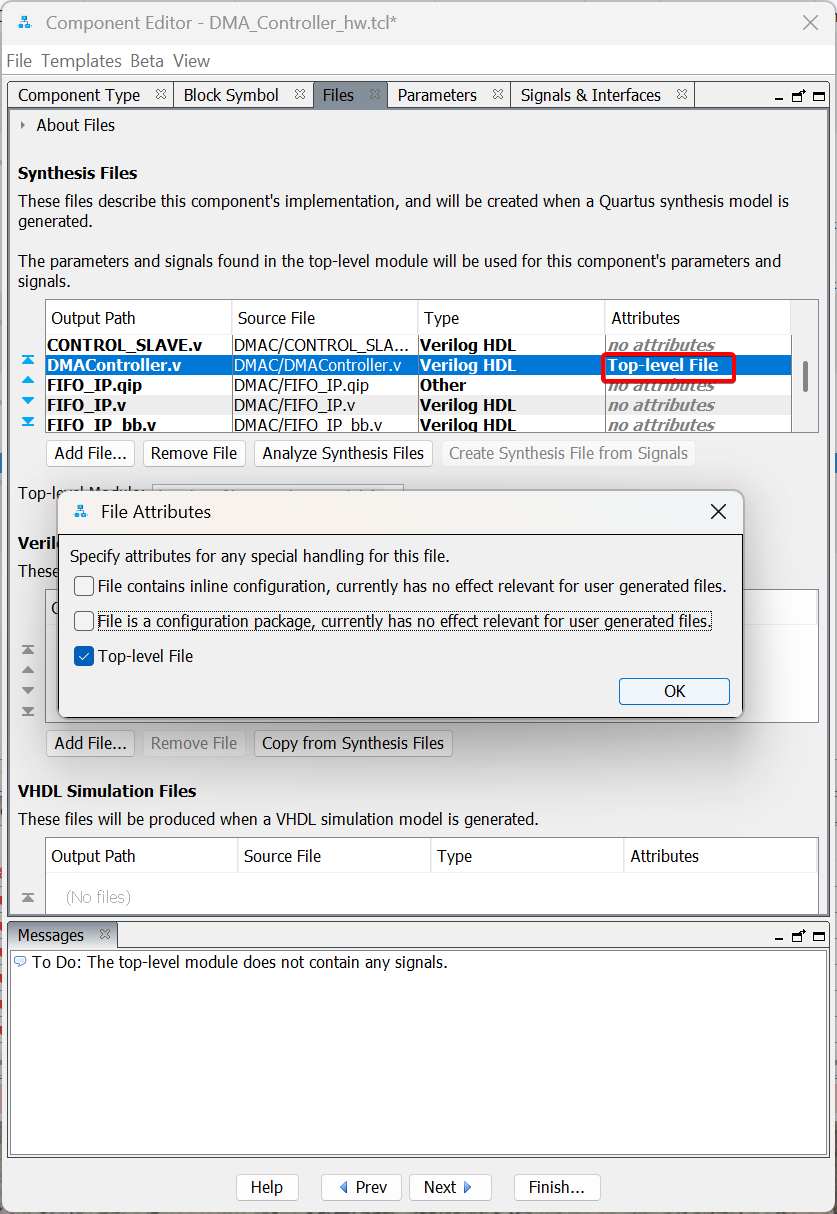
\includegraphics[width=0.9\linewidth]{03_20_ComponentEditorFiles_TopLevel.png} \caption{Component Editor: Thêm tệp Verilog và đặt top-level.} \label{fig:03_20} \end{figure}
\begin{figure}[htbp] \centering 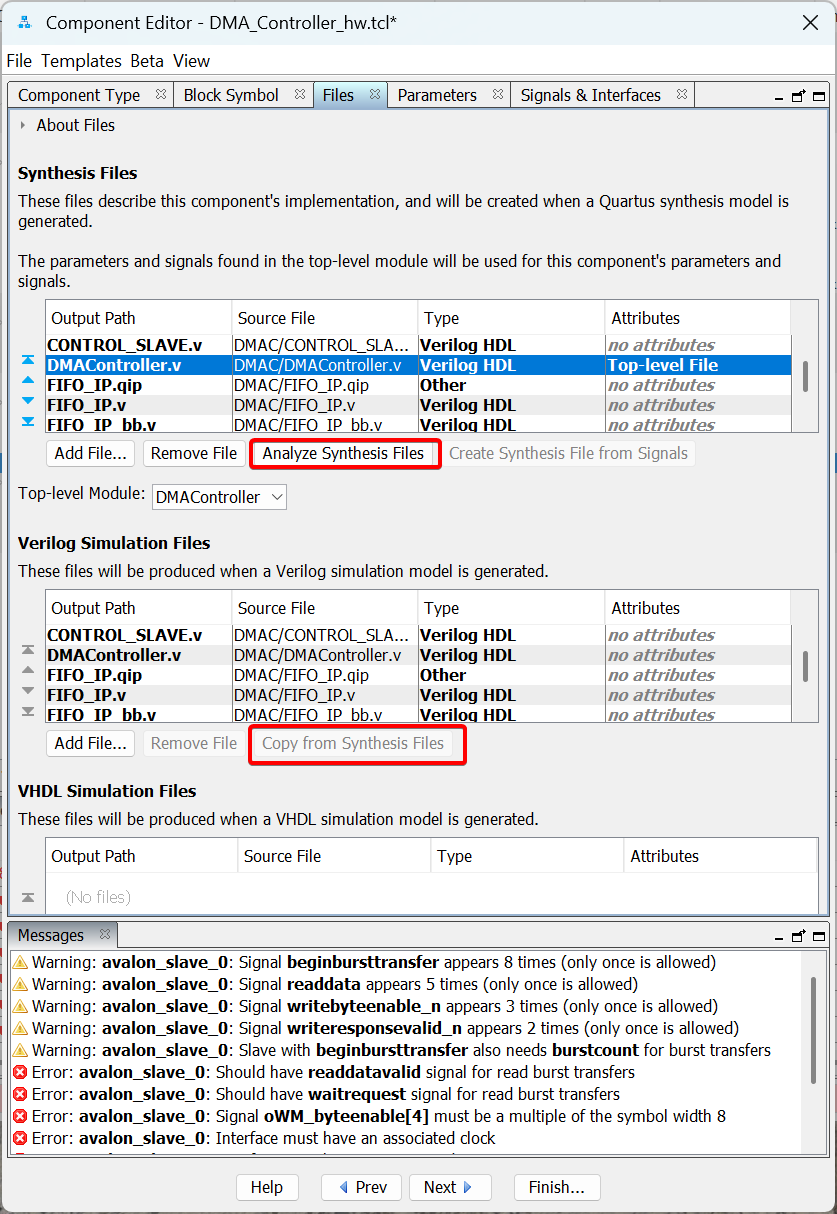
\includegraphics[width=0.9\linewidth]{03_21_ComponentEditorFilesAnalyzed.png} \caption{Component Editor: Các tệp sau khi Phân tích và Sao chép từ Tổng hợp.} \label{fig:03_21} \end{figure}
% \begin{figure}[htbp] \centering 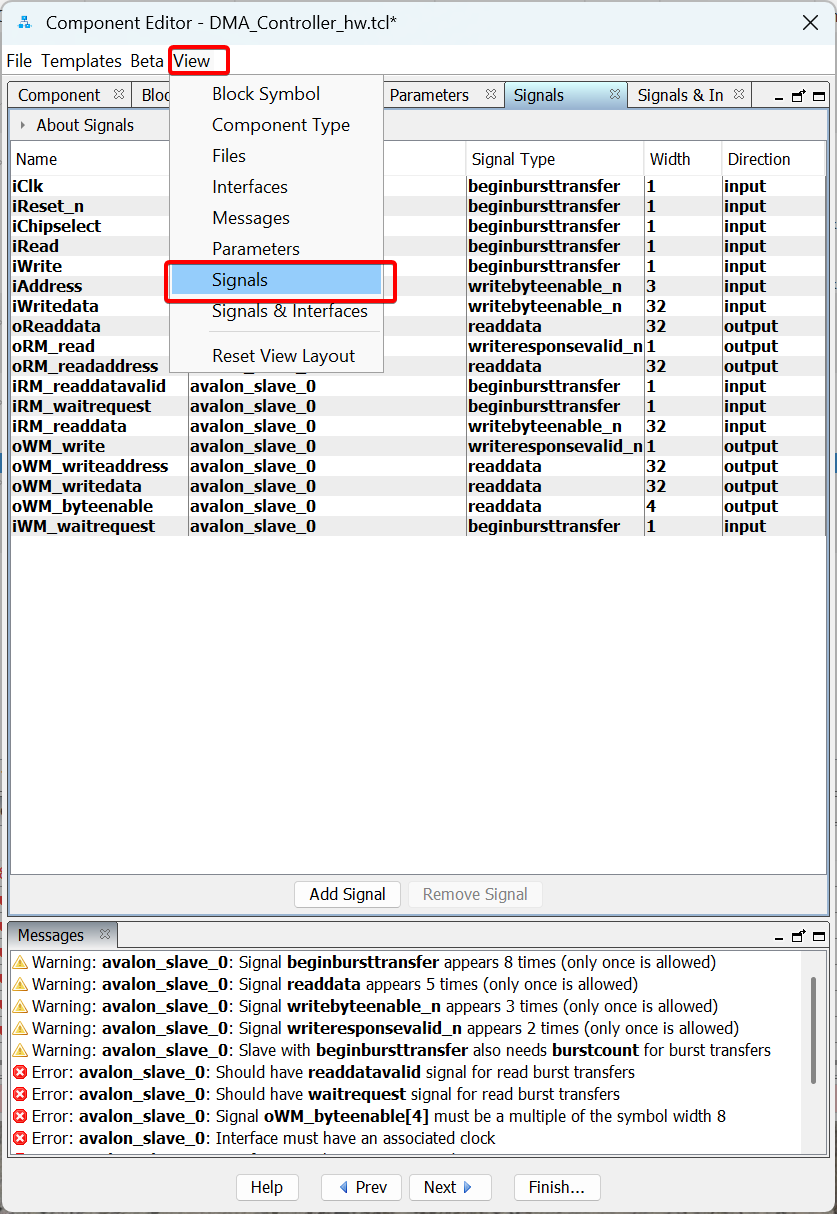
\includegraphics[width=0.9\linewidth]{03_22_ComponentEditorSignals1.png} \caption{Component Editor: Tab Tín hiệu \& Giao diện ban đầu hiển thị cảnh báo.} \label{fig:03_22} \end{figure}
\begin{figure}[htbp] \centering 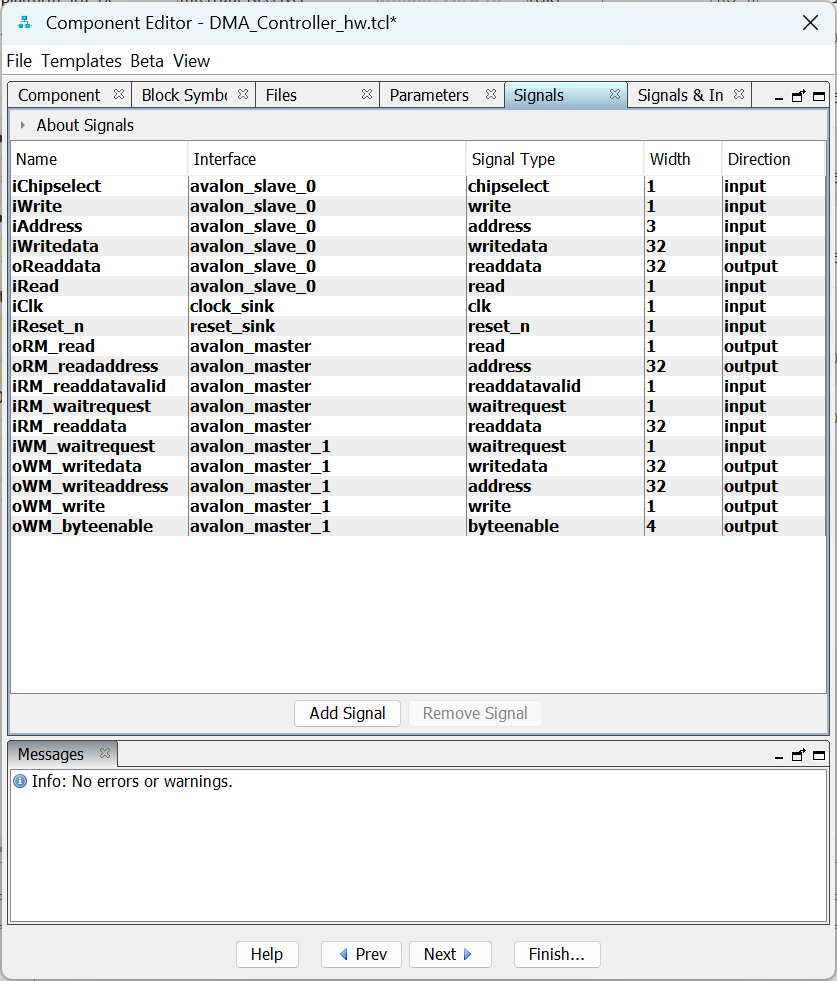
\includegraphics[width=0.9\linewidth]{03_23_ComponentEditorSignals_DMAC.png} \caption{Component Editor: Các loại tín hiệu clock và reset đã được sửa.} \label{fig:03_23} \end{figure}
% \begin{figure}[htbp] \centering 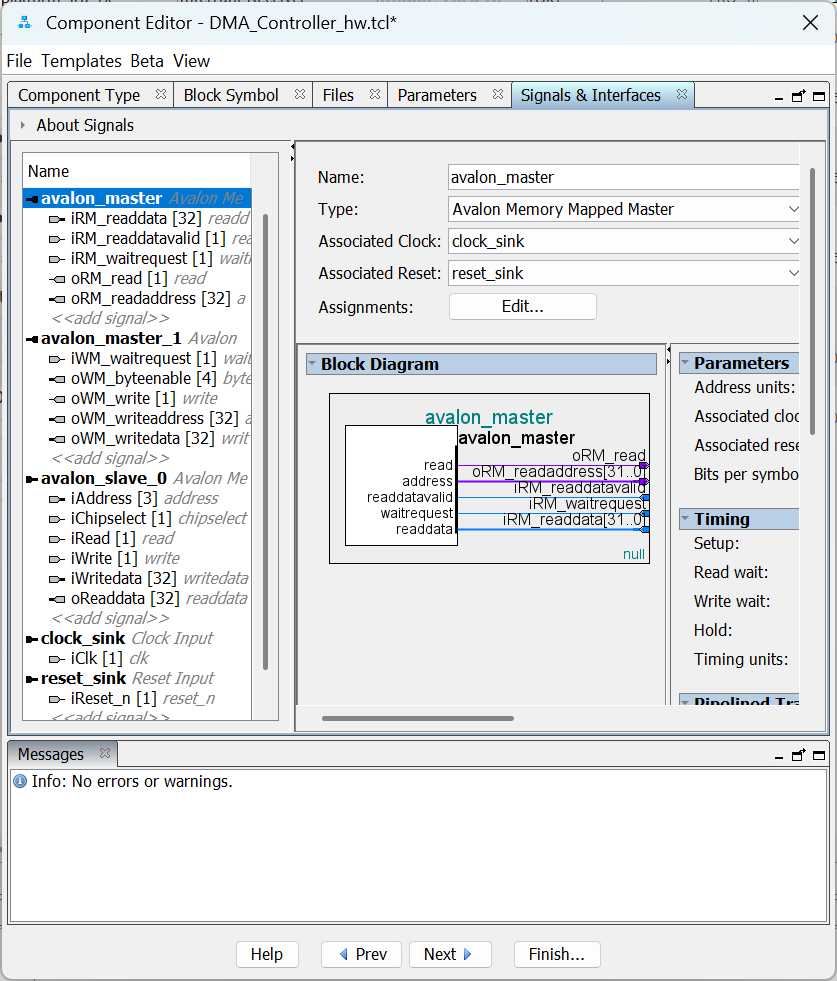
\includegraphics[width=0.5\linewidth]{03_24_ComponentEditorInterfaces1.png} \caption{Component Editor: Định nghĩa giao diện Avalon Master.} \label{fig:03_24} \end{figure}
% \begin{figure}[htbp] \centering 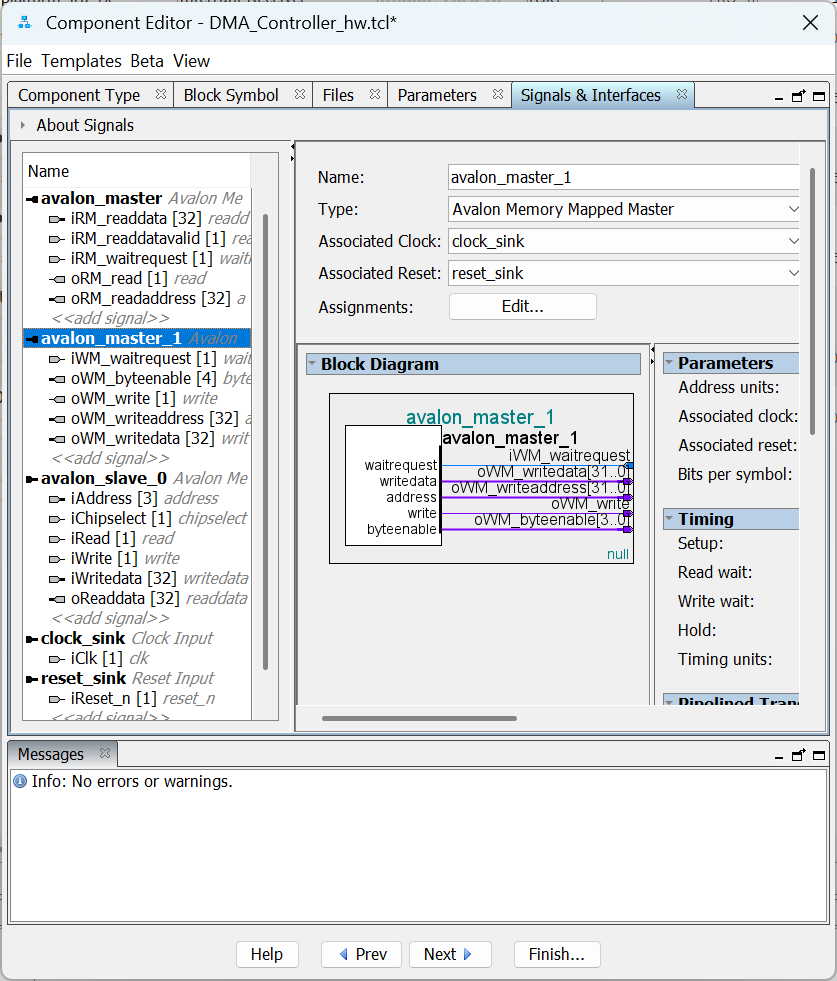
\includegraphics[width=0.5\linewidth]{03_25_ComponentEditorInterfaces2.png} \caption{Component Editor: Chế độ xem sơ đồ khối giao diện Avalon Master.} \label{fig:03_25} \end{figure}
\begin{figure}[htbp] \centering 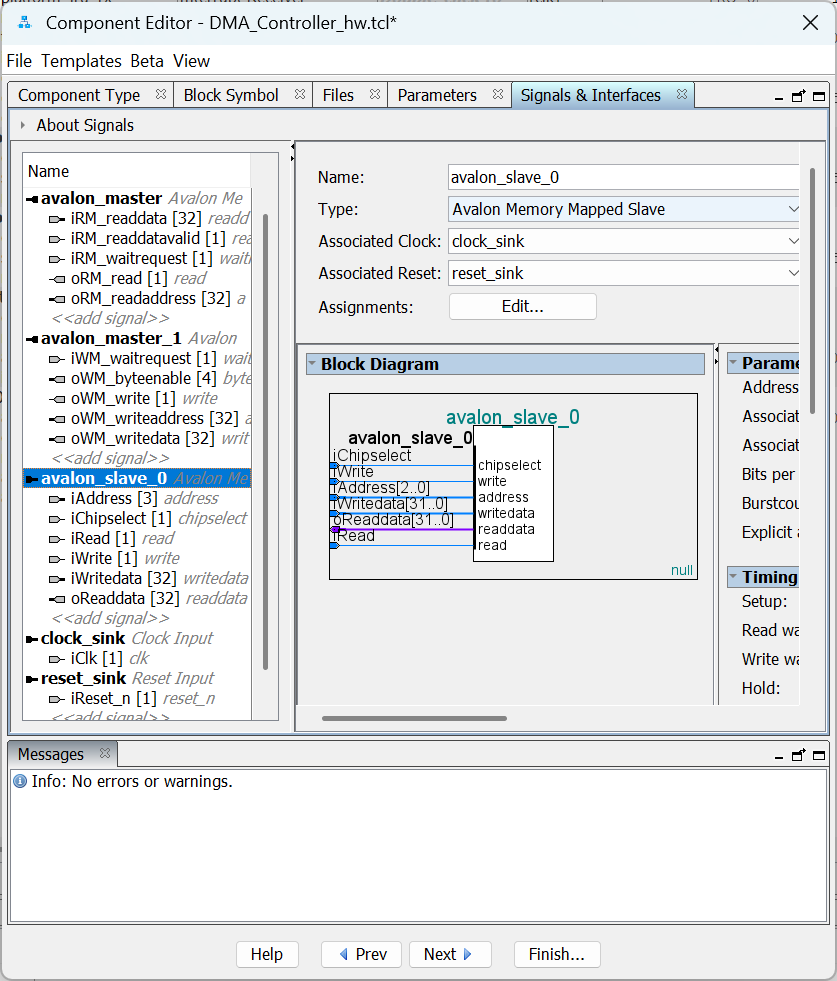
\includegraphics[width=0.5\linewidth]{03_26_ComponentEditorInterfaces3.png} \caption{Component Editor: Chế độ xem sơ đồ khối giao diện Avalon Slave.} \label{fig:03_26} \end{figure}
\begin{figure}[htbp] \centering 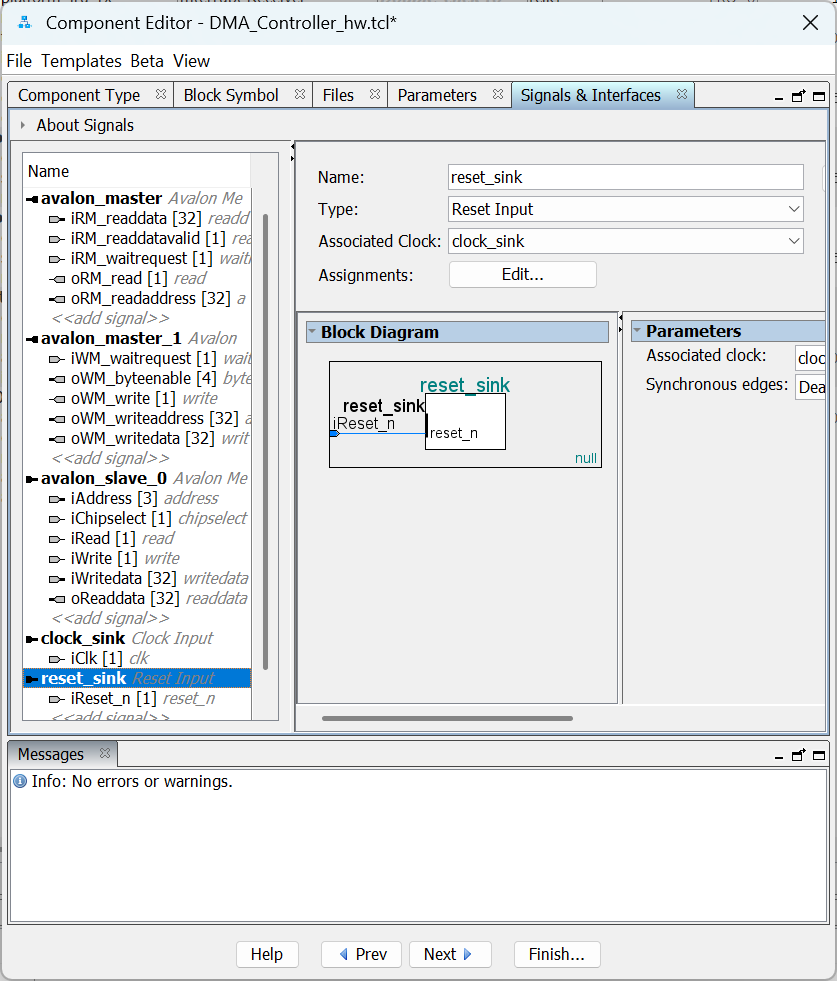
\includegraphics[width=0.5\linewidth]{03_27_ComponentEditorInterfaces4.png} \caption{Component Editor: Chế độ xem giao diện Reset và Clock sink.} \label{fig:03_27} \end{figure}
\begin{figure}[htbp] \centering 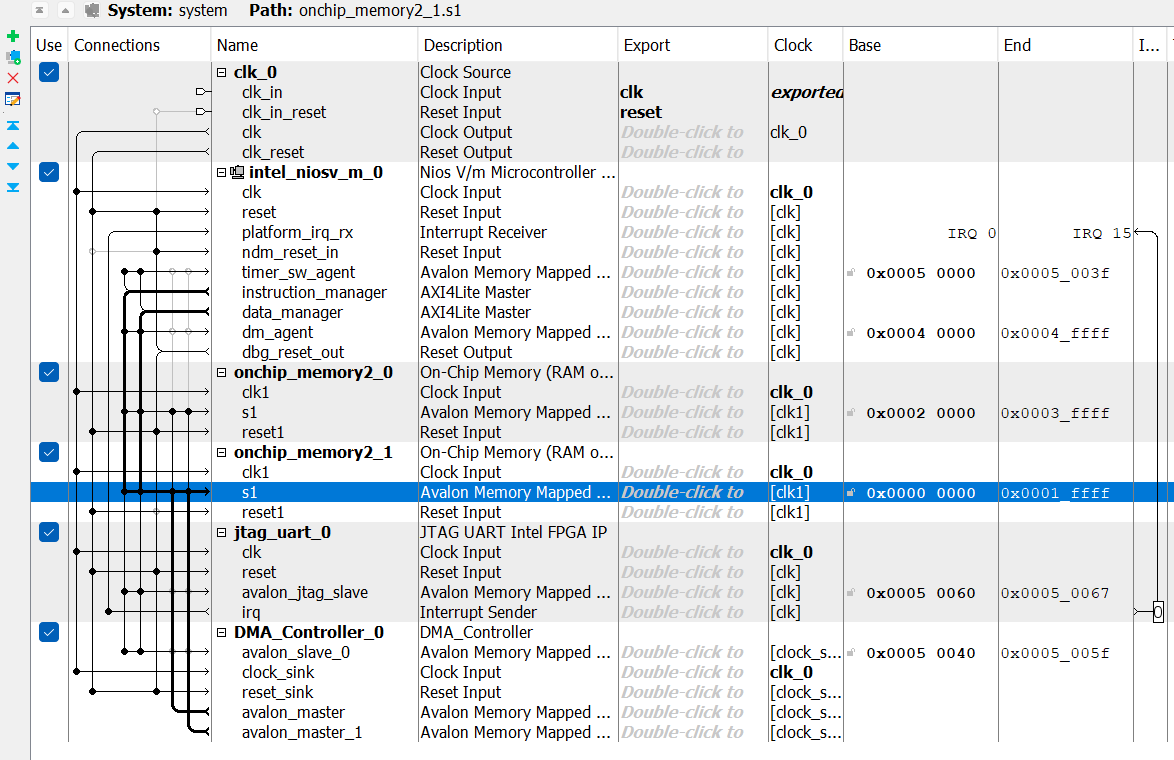
\includegraphics[width=\linewidth]{03_28_PlatformDesignerSystemView1.png} \caption{Platform Designer: Hệ thống có kết nối giữa \texttt{instruction\_master} với s1 (của \texttt{onchip\_memory2\_1}).} \label{fig:03_28} \end{figure}
\begin{figure}[htbp] \centering 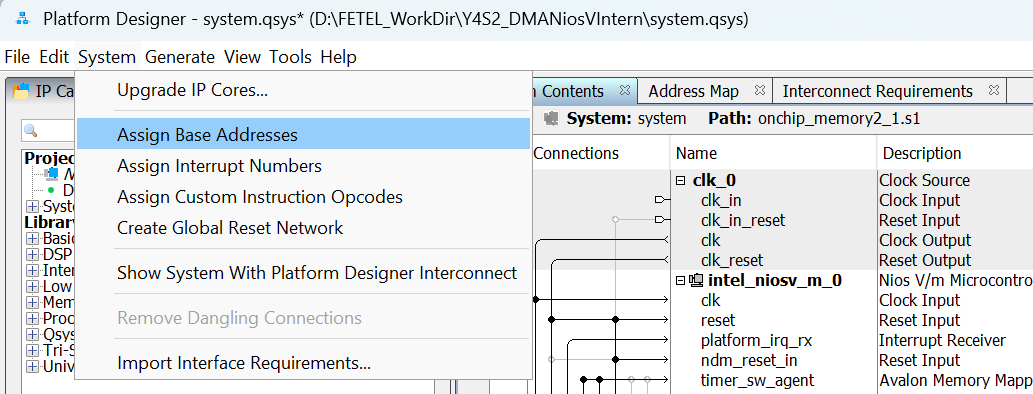
\includegraphics[width=\linewidth]{03_29_PlatformDesignerAssignBaseAddr.png} \caption{Platform Designer: Gán Địa chỉ Cơ sở (Assign Base Addresses).} \label{fig:03_29} \end{figure}
\begin{figure}[htbp] \centering 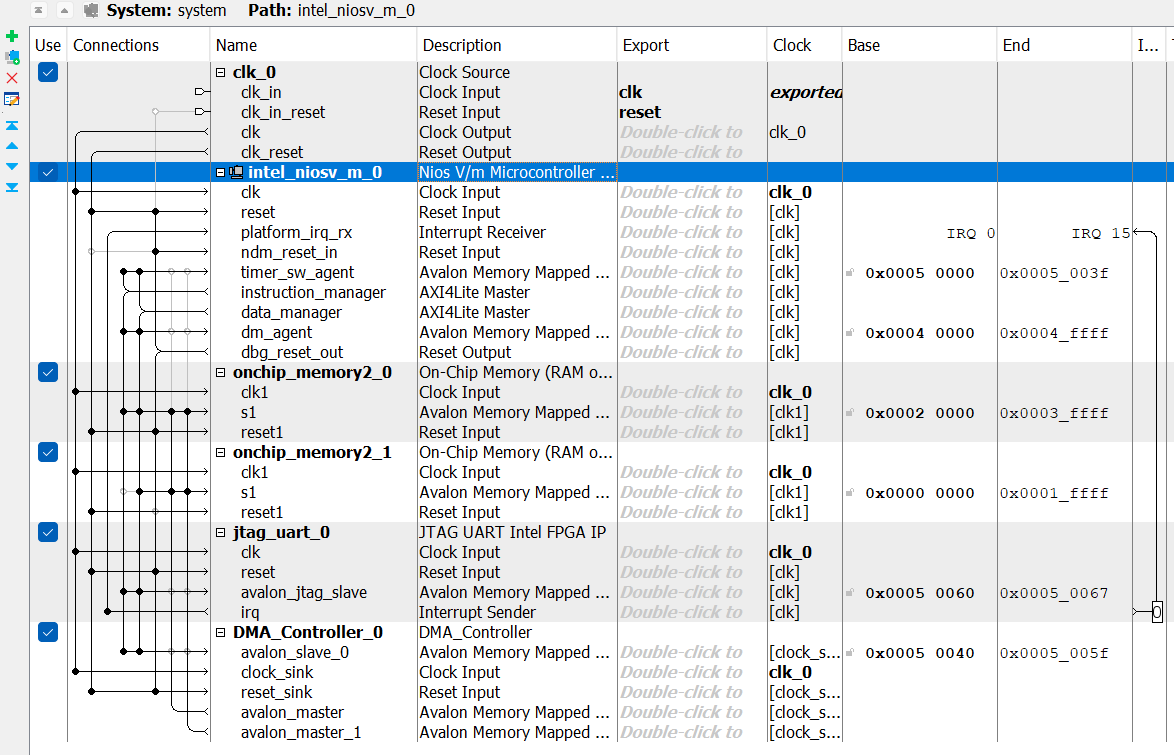
\includegraphics[width=\linewidth]{03_30_PlatformDesignerSystemView_FinalDMAC.png} \caption{Platform Designer: Mô hình hệ thống hoàn chỉnh (sau khi ngắt kết nối \texttt{instruction\_master} với \texttt{s1} trên \texttt{onchip\_memory2\_1}).} \label{fig:03_30} \end{figure}
\begin{figure}[htbp] \centering 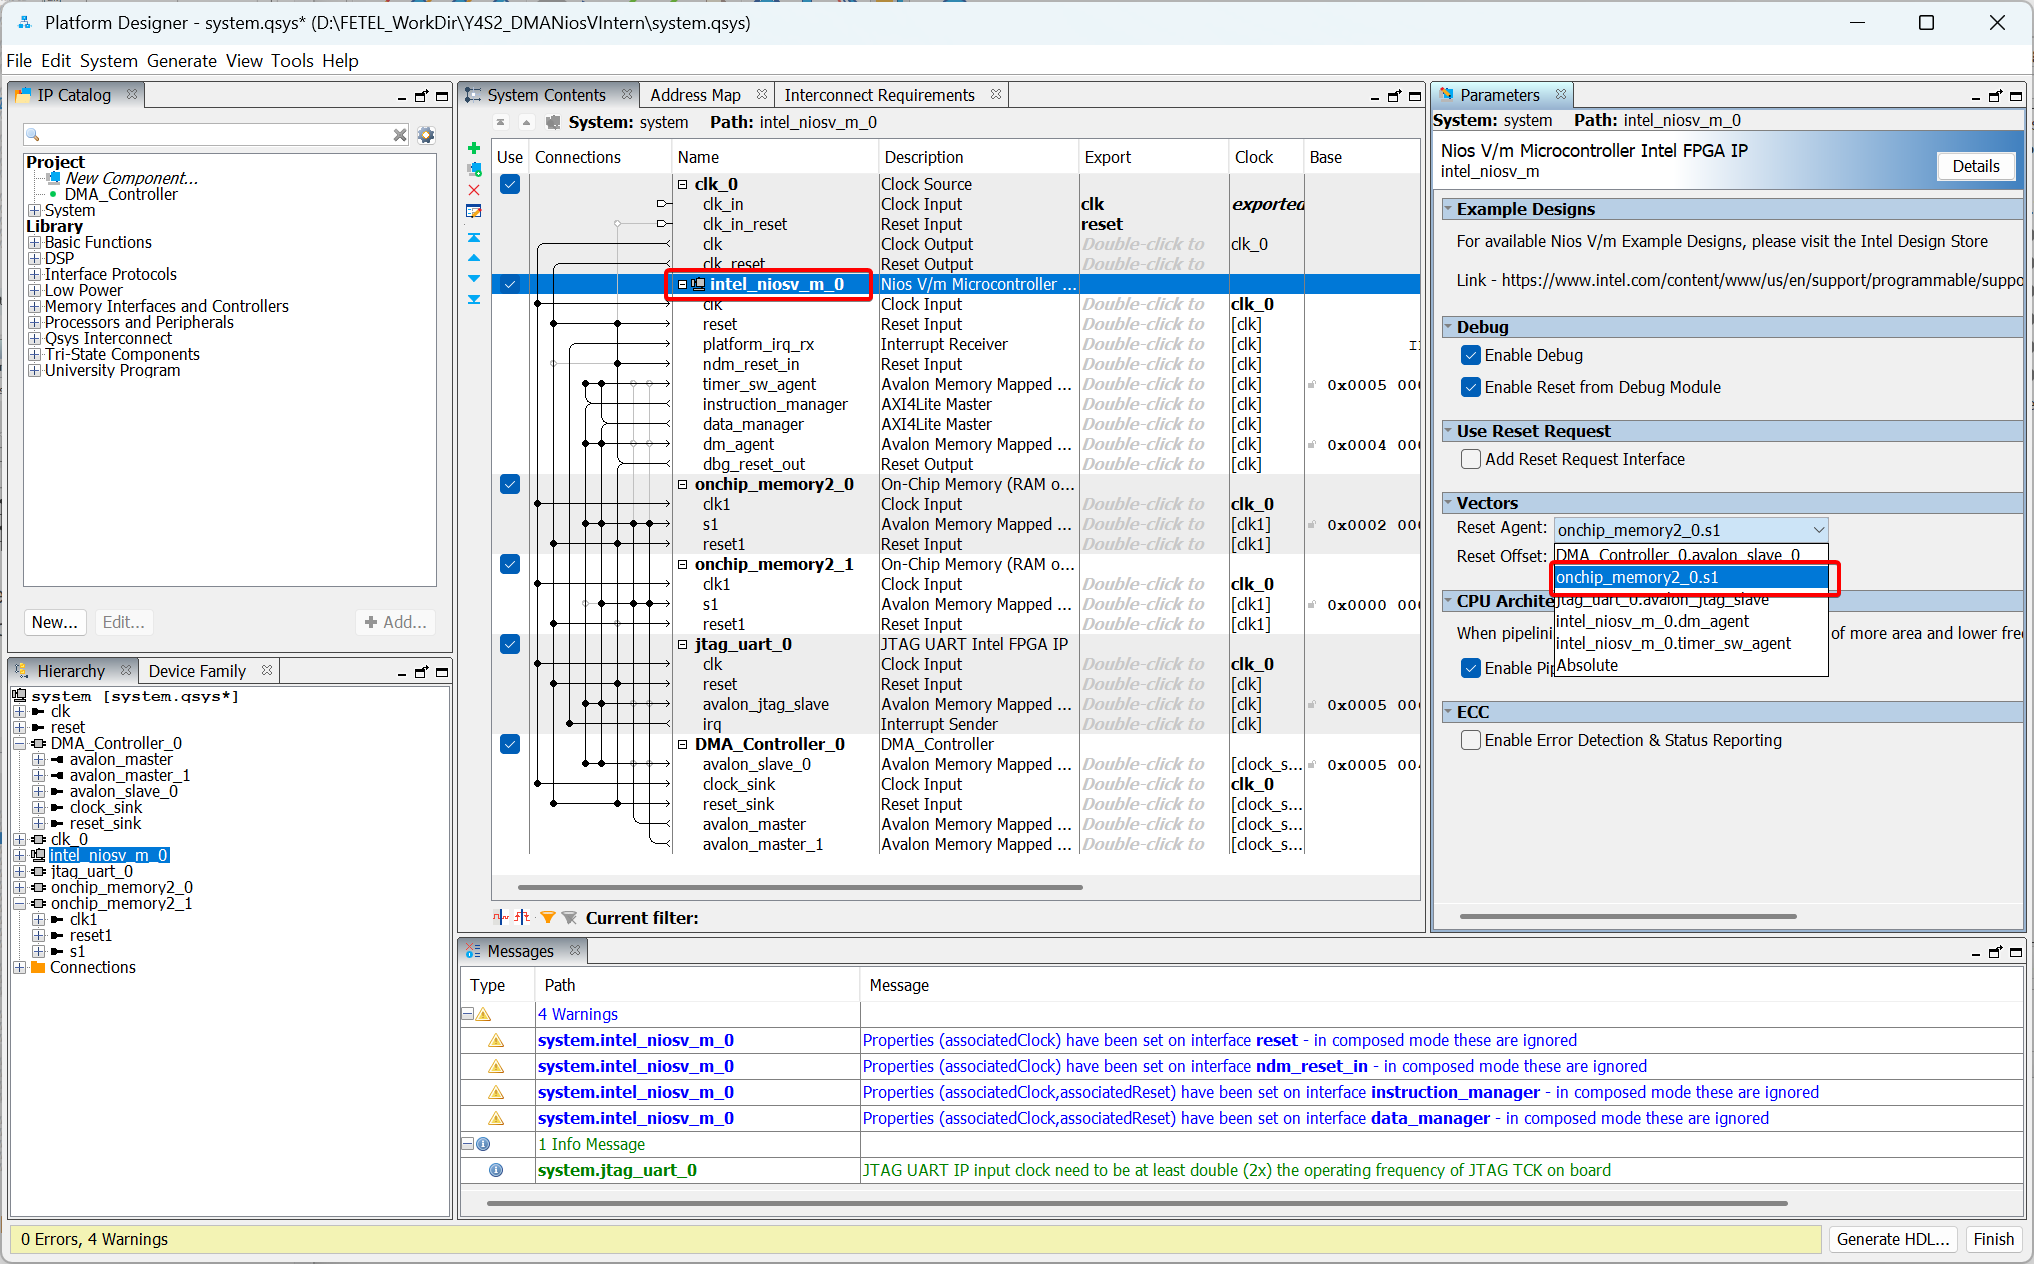
\includegraphics[width=\linewidth]
{03_31_NiosVVectorConfig.png} \caption{Cấu hình IP Nios V/m: Đặt Bộ nhớ Vector Reset (Reset Vector Memory).} \label{fig:03_31} \end{figure}
% \begin{figure}[htbp] \centering 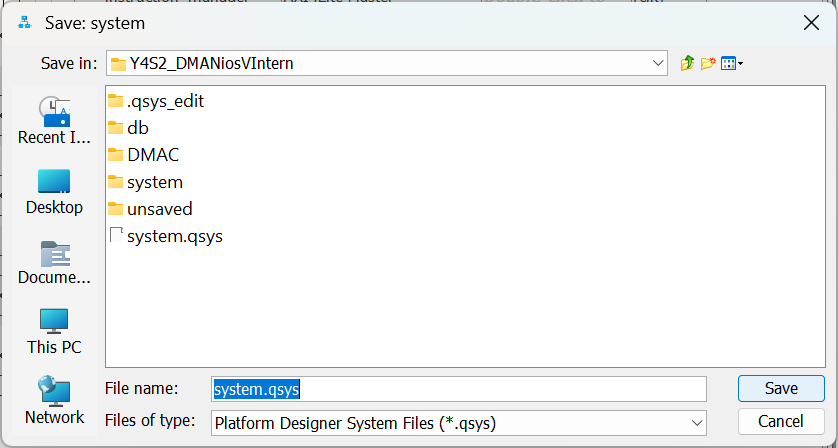
\includegraphics[width=0.5\linewidth]{03_32_PlatformDesignerSaveSystem.png} \caption{Platform Designer: Lưu hệ thống thành system.qsys.} \label{fig:03_32} \end{figure}
% \begin{figure}[htbp] \centering 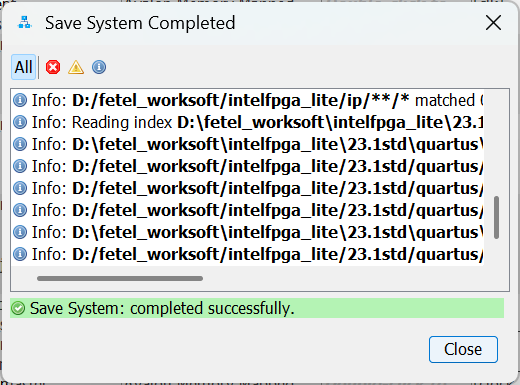
\includegraphics[width=0.5\linewidth]{03_33_PlatformDesignerSaveComplete.png} \caption{Platform Designer: Thông báo lưu hệ thống thành công.} \label{fig:03_33} \end{figure}
\begin{figure}[htbp] \centering 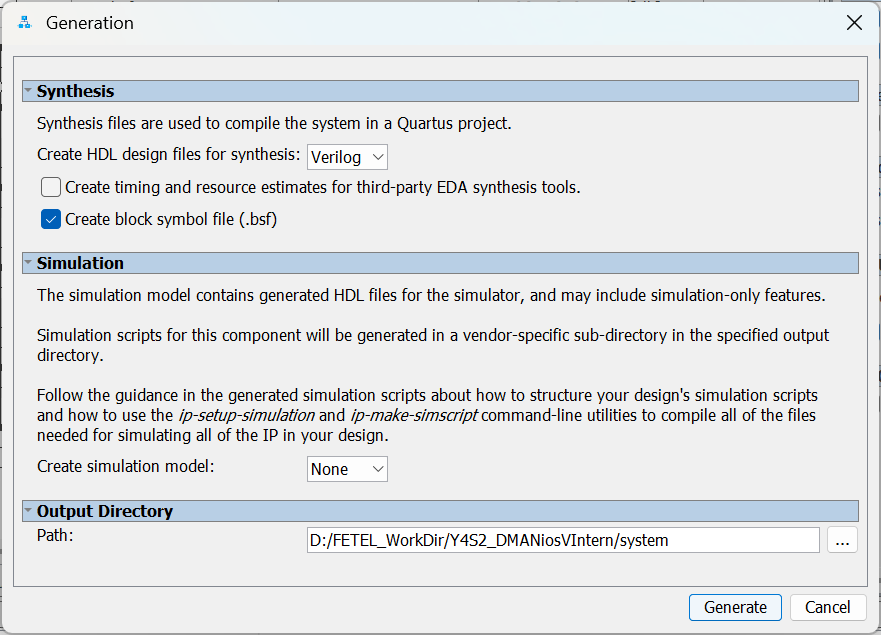
\includegraphics[width=0.7\linewidth]{03_34_PlatformDesignerGenerateHDL.png} \caption{Platform Designer: Hộp thoại Tạo HDL (Generate HDL).} \label{fig:03_34} \end{figure}
% \begin{figure}[htbp] \centering 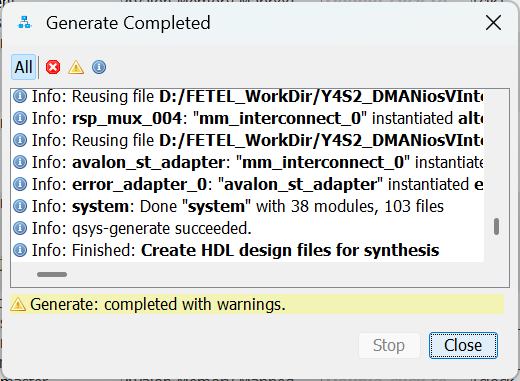
\includegraphics[width=0.4\linewidth]{03_35_PlatformDesignerGenerateComplete.png} \caption{Platform Designer: Thông báo hoàn thành tạo HDL.} \label{fig:03_35} \end{figure}
% \begin{figure}[htbp] \centering 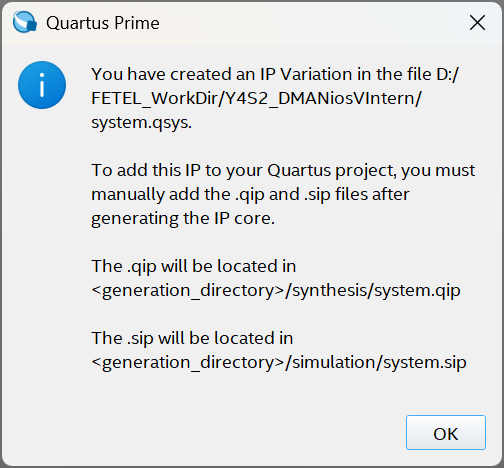
\includegraphics[width=0.4\linewidth]{03_36_QuartusAddGeneratedIPInfo.png} \caption{Quartus: Thông báo đề xuất thêm tệp .qip đã tạo.} \label{fig:03_36} \end{figure}
\begin{figure}[htbp] \centering 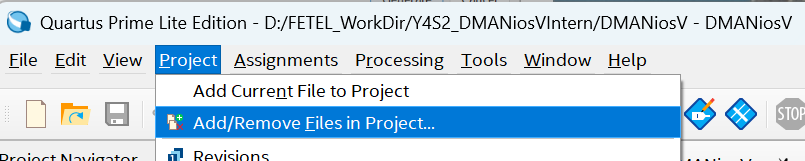
\includegraphics[width=0.8\linewidth]{03_37_QuartusAddFilesToProjectMenu.png} \caption{Quartus: Menu Project -> Add/Remove Files in Project...} \label{fig:03_37} \end{figure}
\begin{figure}[htbp] \centering 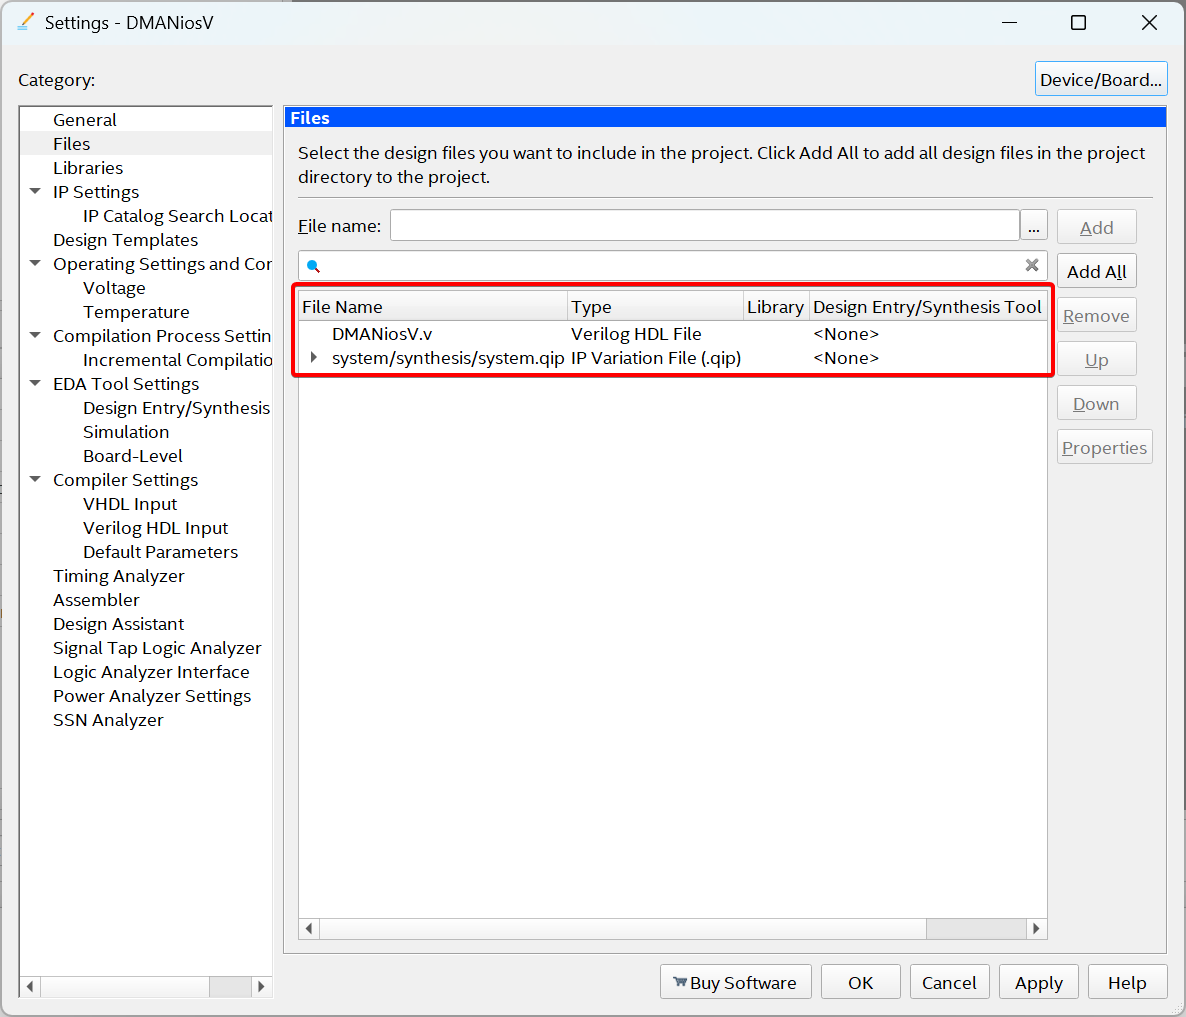
\includegraphics[width=0.7\linewidth]{03_38_QuartusProjectFilesSettings.png} \caption{Quartus: Cài đặt Dự án - Cửa sổ Tệp hiển thị tệp .qip đã thêm.} \label{fig:03_38} \end{figure}
\begin{figure}[htbp] \centering 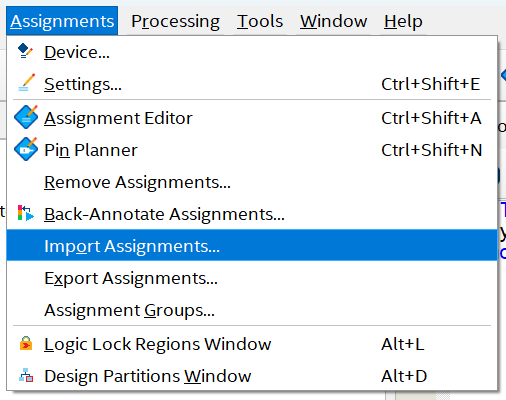
\includegraphics[width=0.5\linewidth]{03_39_QuartusImportAssignmentsMenu.png} \caption{Quartus: Menu Assignments -> Import Assignments...} \label{fig:03_39} \end{figure}
\begin{figure}[htbp] \centering 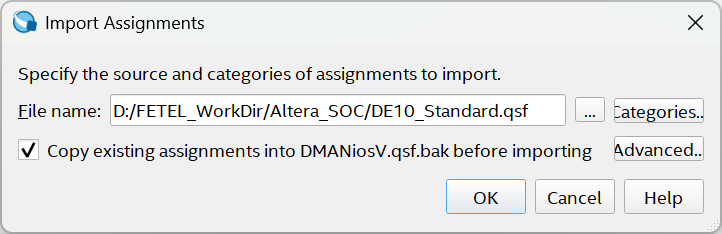
\includegraphics[width=0.5\linewidth]{03_40_QuartusImportAssignmentsDialog.png} \caption{Quartus: Hộp thoại Nhập Gán chân (Import Assignments) để chọn tệp .qsf.} \label{fig:03_40} \end{figure}
\begin{figure}[htbp] \centering 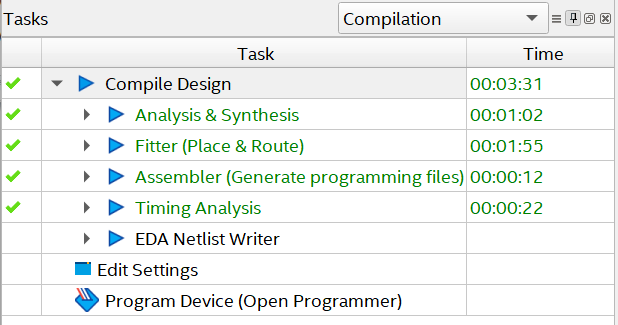
\includegraphics[width=0.6\linewidth]{03_41_QuartusCompilationTasks.png} \caption{Quartus: Compile Design thành công.} \label{fig:03_41} \end{figure}
\begin{figure}[htbp] \centering 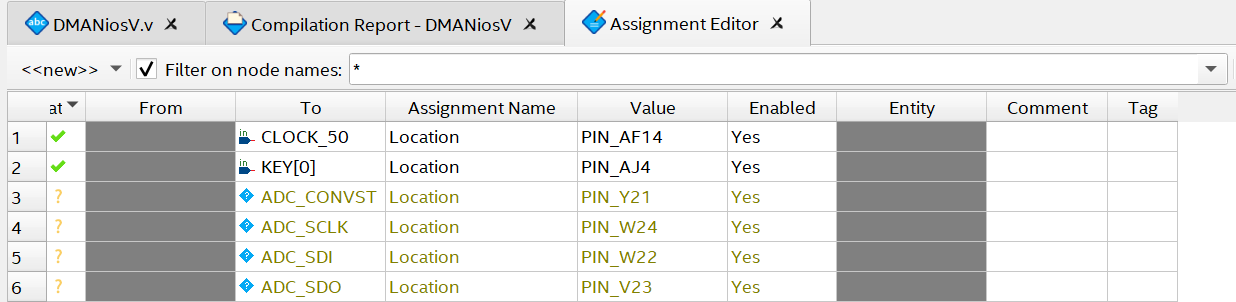
\includegraphics[width=\linewidth]{03_42_QuartusAssignmentEditor.png} \caption{Quartus: Trình chỉnh sửa Gán chân (Assignment Editor) hiển thị các gán chân đã nhập.} \label{fig:03_42} \end{figure}

\FloatBarrier

\subsection{Phát triển Ứng dụng Phần mềm Nios V}
\label{sec:develop_software}

Phần này mô tả việc tạo Gói Hỗ trợ Bo mạch (Board Support Package - \acrshort{bsp}) và mã ứng dụng C, sau đó biên dịch và gỡ lỗi (debug) nó bằng \acrshort{ide} Ashling RiscFree.

\begin{enumerate}
    \item \textbf{Chuẩn bị Cấu trúc Thư mục Phần mềm:} Tạo một thư mục \texttt{software} trong thư mục dự án chính (\texttt{DMANiosVIntern}). Bên trong \texttt{software}, tạo hai thư mục con: \texttt{app} và \texttt{bsp} (Hình \ref{fig:03_43}). Đặt mã nguồn ứng dụng C của bạn (ví dụ: \texttt{source.c} chứa logic kiểm thử DMA) vào bên trong thư mục \texttt{app} (Hình \ref{fig:03_45}).
    \item \textbf{Tạo BSP và Tệp CMake:}
    \begin{itemize}
        \item Mở Nios V command shell (\texttt{niosv-shell.exe}) nằm trong thư mục cài đặt Intel FPGA (ví dụ: \texttt{intelFPGA\_lite/23.1std/niosv/bin}) (Hình \ref{fig:03_46}).
        \item Điều hướng Nios V Shell đến thư mục dự án (Working Directory, \ref{fig:03_11}): 
        \begin{lstlisting}[language=bash, caption={Điều hướng trong Nios V Shell}, label=lst:cd_project] 
        cd D:\FETEL_WorkDir\Y4S2_DMANiosVIntern \end{lstlisting}
        \item Tạo \acrshort{bsp} bằng lệnh \texttt{niosv-bsp}. Lệnh này sử dụng tệp thông tin phần cứng (\texttt{.sopcinfo}) được tạo bởi Platform Designer để tạo các trình điều khiển (drivers) và các tệp tiêu đề hệ thống (system headers) \cite{intelNiosVSoftwareDevHandbook}:
        \begin{lstlisting}[language=bash, caption={Lệnh tạo BSP Nios V}, label=lst:gen_bsp]
# -c: create BSP, -t=hal: type HAL, --sopcinfo: path to hardware info
niosv-bsp -c -t=hal --sopcinfo=system.sopcinfo software/bsp/settings.bsp \end{lstlisting}
        \item Tạo các tệp xây dựng CMake cho ứng dụng bằng \texttt{niosv-app}. Lệnh này liên kết nguồn ứng dụng (\texttt{-a}) với \acrshort{bsp} đã tạo (\texttt{-b}) và chỉ định thư mục nguồn (\texttt{-s}) \cite{intelNiosVSoftwareDevHandbook}:
        \begin{lstlisting}[language=bash, caption={Lệnh tạo tệp CMake ứng dụng Nios V}, label=lst:gen_app]
# -a: app dir, -b: bsp dir, -s: source dir (relative to app dir)
niosv-app -a=software/app -b=software/bsp -s=software/app \end{lstlisting}
        (Xem Hình \ref{fig:03_47} cho việc thực thi lệnh và Hình \ref{fig:03_48} cho đầu ra tạo BSP). Đảm bảo không có lỗi xảy ra. Một tệp \texttt{CMakeLists.txt} bây giờ sẽ tồn tại trong thư mục \texttt{software/app}.
    \end{itemize}
    \item \textbf{Xây dựng Ứng dụng bằng Ashling RiscFree™ IDE \cite{ashling_riscfree_guide}:}
    \begin{itemize}
        \item \textbf{Khởi chạy IDE:} Quan trọng là khởi chạy Ashling RiscFree™ IDE từ \texttt{ niosv-shell.exe} bằng cách gõ \texttt{riscfree}. Điều này đảm bảo các biến môi trường (environment variables) được thiết lập chính xác (Hình \ref{fig:03_49}).
        \item \textbf{Chọn Workspace:} Chọn thư mục \texttt{software} (Hình \ref{fig:03_50}).
        \item \textbf{Import Project:} Trong IDE (Hình \ref{fig:03_51}), đi đến File -> New -> C/C++ Project (Hình \ref{fig:03_52}). Chọn "C Project". Đặt tên dự án là \texttt{app} (trùng với tên thư mục). Chọn "Empty Project" dưới loại dự án "CMake driven" (Hình \ref{fig:03_53}). Nhấp Finish. IDE sẽ phát hiện \texttt{CMakeLists.txt} và cấu hình dự án.
        \item \textbf{Xây dựng Dự án (Build Project):} Nhấp chuột phải vào dự án \texttt{app} trong Trình khám phá Dự án (Project Explorer) (Hình \ref{fig:03_54}) và chọn "Build Project" (hoặc sử dụng Ctrl+B) (Hình \ref{fig:03_55}). Kiểm tra cửa sổ Console để xem tiến trình xây dựng và đảm bảo nó hoàn thành mà không có lỗi (Hình \ref{fig:03_56}). Thao tác này tạo ra tệp thực thi (\texttt{app.elf}) bên trong một thư mục xây dựng (ví dụ: \texttt{software/app/build/Debug}). 
    \end{itemize}
    \item \textbf{Nạp chương trình cho FPGA và Chạy/Gỡ lỗi Phần mềm:}
    \begin{itemize}
        \item \textbf{Nạp chương trình cho FPGA (Program FPGA):} Sử dụng Quartus Programmer (Tools -> Programmer) để tải thiết kế phần cứng đã biên dịch (tệp \texttt{.sof} từ mục \ref{sec:build_hardware}) lên bo mạch DE10-Standard thông qua kết nối \acrshort{usb}-Blaster. Đảm bảo phần cứng đã được kết nối và bắt đầu quá trình nạp (Hình \ref{fig:03_59}).
        \item \textbf{Cấu hình Trình gỡ lỗi (Configure Debugger):} Trong Ashling IDE, nhấp chuột phải vào dự án \texttt{app} -> Run As -> Ashling RISC-V Hardware Debugging... (Hình \ref{fig:03_60}). Chọn app.elf (Hình \ref{fig:03_61}).
        \begin{itemize}
            \item Chuyển đến tab "Debugger". Chọn Đầu dò Gỡ lỗi (Debug Probe) chính xác (ví dụ: "DE-SoC [\acrshort{usb}-1]"). Đảm bảo "Lựa chọn Thiết bị/TAP (Device/TAP selection)" khớp với lõi Nios V được xác định trên chuỗi \acrshort{jtag} (sử dụng "Auto-detect Scan Chain" nếu không chắc chắn). Loại Vận chuyển (Transport type) phải là \acrshort{jtag} (Hình \ref{fig:03_62}). Áp dụng (Apply) và nhấp Debug.
        \end{itemize}
        \item \textbf{Chạy và Quan sát (Run and Observe):} IDE sẽ kết nối với lõi Nios V, tải xuống tệp \texttt{.elf}, và dừng tại đầu hàm \texttt{main()} (Hình \ref{fig:03_63}). Mở một \texttt{juart-terminal} trong Nios V shell để xem đầu ra (output) của chương trình:
        \begin{lstlisting}[language=bash, caption={Khởi chạy JTAG UART Terminal}, label=lst:juart]
juart-terminal \end{lstlisting}
        \item Quan sát đầu ra trong cửa sổ \texttt{juart-terminal} (Hình \ref{fig:03_64}, \ref{fig:03_65}, \ref{fig:03_66}). Đầu ra ví dụ cho thấy các thanh ghi DMA đang được cấu hình, trạng thái đang được thăm dò (polling), bộ đệm bộ nhớ đang được xóa/xả (cleared/flushed), và cuối cùng, xác minh rằng việc truyền dữ liệu qua DMA đã diễn ra chính xác.
    \end{itemize}
\end{enumerate}

% Figure environments for Section 3.3
\begin{figure}[htbp] \centering 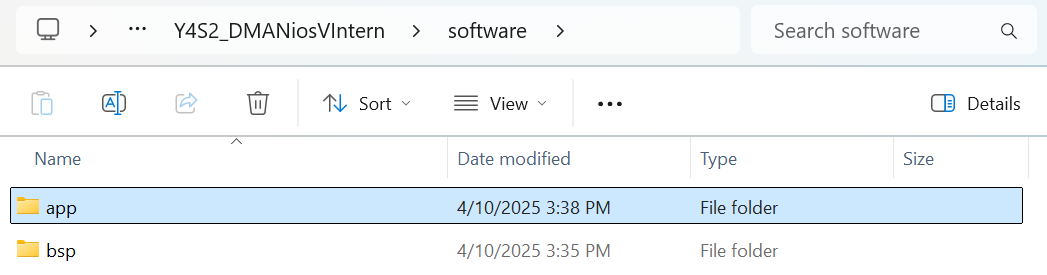
\includegraphics[width=0.8\linewidth]{03_43_SoftwareFoldersAppBSP.png} \caption{Cấu trúc thư mục Software gồm các thư mục con \texttt{app} và \texttt{bsp}.} \label{fig:03_43} \end{figure}
\begin{figure}[htbp] \centering 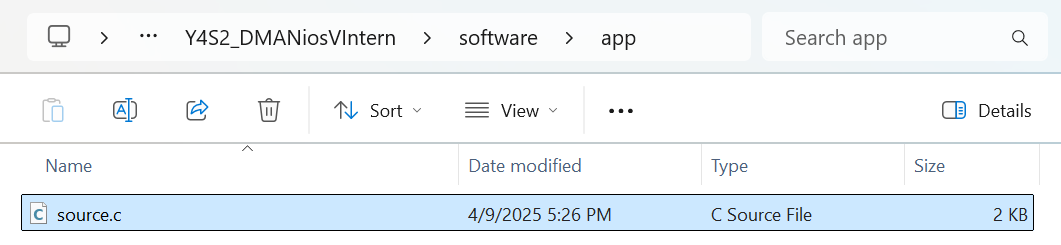
\includegraphics[width=0.8\linewidth]{03_45_SoftwareAppFolderSourceC.png} \caption{Thư mục \texttt{software/app} chứa tệp mã nguồn \texttt{source.c}.} \label{fig:03_45} \end{figure}
\begin{figure}[htbp] \centering 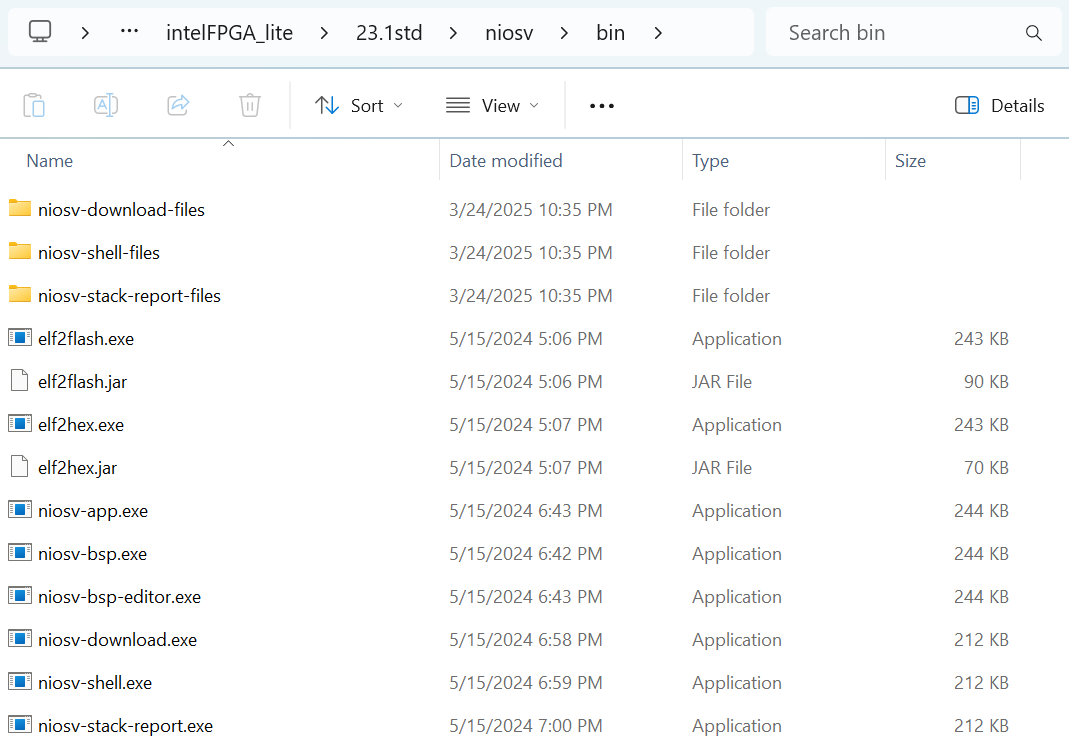
\includegraphics[width=0.8\linewidth]{03_46_NiosVShellLocation.png} \caption{Vị trí của \texttt{niosv-shell.exe}.} \label{fig:03_46} \end{figure}
\begin{figure}[htbp] \centering 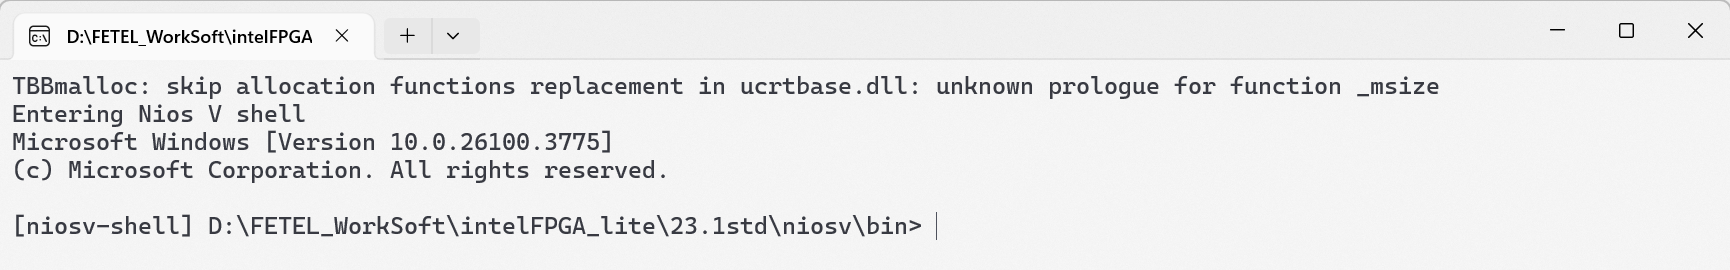
\includegraphics[width=\linewidth]{03_47_NiosVShellCommands.png} \caption{Cửa sổ Nios V Shell.} \label{fig:03_47} \end{figure}
\begin{figure}[htbp] \centering \includegraphics[width=\linewidth]{03_48_NiosVShellBSPOutput.png} \caption{Đầu ra từ việc thực thi lệnh \texttt{niosv-bsp}.} \label{fig:03_48} \end{figure}\begin{figure}[htbp] \centering \includegraphics[width=0.9\linewidth]{03_49_NiosVShellAppOutput.png} \caption{Đầu ra từ việc thực thi lệnh \texttt{niosv-app}.} \label{fig:03_49} \end{figure}
\begin{figure}[htbp] \centering \includegraphics[width=\linewidth]{03_50_AshlingRiscFreefromNiosVShell.png} \caption{Khởi chạy Ashling RiscFree™ IDE từ Nios V Shell, chọn đường dẫn Workspace.} \label{fig:03_50} \end{figure}
\begin{figure}[htbp] \centering \includegraphics[width=0.8\linewidth]{03_51_AshlingRiscFreeLauncher2.png} \caption{Màn hình chào mừng Ashling RiscFree™ IDE: Chọn "Create a project...".} \label{fig:03_51} \end{figure}
\begin{figure}[htbp] \centering \includegraphics[width=0.8\linewidth]{03_52_AshlingIDEWelcome.png} \caption{Ashling IDE: Chọn C/C++ $\longrightarrow$ C Project.} \label{fig:03_52} \end{figure}
\begin{figure}[htbp] \centering \includegraphics[width=0.8\linewidth]{03_53_AshlingIDENewProjectWizard1.png} \caption{Ashling IDE: Chọn CMake driven $\longrightarrow$ Empty Project.} \label{fig:03_53} \end{figure}
\begin{figure}[htbp] \centering \includegraphics[width=0.8\linewidth]{03_54_AshlingIDENewProjectWizard2.png} \caption{Ashling IDE: Project Explorer hiển thị dự án 'app'.} \label{fig:03_54} \end{figure}
\begin{figure}[htbp] \centering \includegraphics[width=0.4\linewidth]{03_55_AshlingIDEProjectExplorer.png} \caption{Ashling IDE: nhấp chuột phải 'app' $\longrightarrow$ Build Project.} \label{fig:03_55} \end{figure}
\begin{figure}[htbp] \centering \includegraphics[width=\linewidth]{03_56_AshlingIDEBuildMenu.png} \caption{Ashling IDE: Console thông báo Build thành công.} \label{fig:03_56} \end{figure}
% \begin{figure}[htbp] \centering \includegraphics[width=0.8\linewidth]{03_57_AshlingIDEBuildConsole.png} \caption{Ashling IDE: Tab Problems không có lỗi.} \label{fig:03_57} \end{figure}
% \begin{figure}[htbp] \centering \includegraphics[width=0.6\linewidth]{03_58_QuartusProgrammerSetup.png} \caption{Trình lập trình Quartus: Cửa sổ Cài đặt Phần cứng (Hardware Setup) hiển thị DE-SoC đã được nhận.} \label{fig:03_58} \end{figure}
\begin{figure}[htbp] \centering \includegraphics[width=0.7\linewidth]{03_59_QuartusProgrammerWindow.png} \caption{Quartus Programmer: Nạp tệp .sof xuống board thành công.} \label{fig:03_59} \end{figure}
\begin{figure}[htbp] \centering \includegraphics[width=0.8\linewidth]{03_60_AshlingIDEDebugMenu.png} \caption{Ashling IDE: Nạp Firmware xuống lõi Nios V (Run As $\longrightarrow$ Ashling RISC-V Hardware Debugging.} \label{fig:03_60} \end{figure}
\begin{figure}[htbp] \centering \includegraphics[width=0.4\linewidth]{03_61_AshlingIDERunConfigELF.png} \caption{Ashling IDE: Cấu hình Gỡ lỗi - Chỉ định ứng dụng C/C++ (.elf).} \label{fig:03_61} \end{figure}
\begin{figure}[htbp] \centering \includegraphics[width=\linewidth]{03_62_AshlingIDEDebugConfig.png} \caption{Ashling IDE: Cấu hình Gỡ lỗi - Cài đặt tab Debugger.} \label{fig:03_62} \end{figure}
\begin{figure}[htbp] \centering \includegraphics[width=\linewidth]{03_63_AshlingIDEDebugConsole.png} \caption{Ashling IDE: Debug Console cho biết đang chờ kết nối (Nhấn nút đỏ để ngừng chạy).} \label{fig:03_63} \end{figure}
\begin{figure}[htbp] \centering \includegraphics[width=0.8\linewidth]{03_64_JUARTTerminalOutput1.png} \caption{Đầu ra JTAG UART Terminal: Thông báo ban đầu và reset DMA.} \label{fig:03_64} \end{figure}
\begin{figure}[htbp] \centering \includegraphics[width=0.8\linewidth]{03_65_JUARTTerminalOutput2.png} \caption{Đầu ra JTAG UART Terminal: Trạng thái bộ đệm và cấu hình DMA.} \label{fig:03_65} \end{figure}
\begin{figure}[htbp] \centering \includegraphics[width=0.7\linewidth]{03_66_JUARTTerminalOutput3.png} \caption{Đầu ra JTAG UART Terminal: Xác minh truyền DMA thành công.} \label{fig:03_66} \end{figure}

\FloatBarrier

% Platform Designer có thể tạo ra các mô hình mô phỏng (simulation models) (Hình \ref{fig:03_34}), nhưng việc tạo ra một hệ thống bàn thử nghiệm (testbench system) đầy đủ, đặc biệt là liên quan đến các mô hình bộ xử lý như Nios V/g, có thể phức tạp và đôi khi gặp hạn chế về công cụ trên hệ điều hành Windows cho việc tạo testbench \cite{intel-forum-simulation}.

% Note: Appendix content moved to appendix1.tex as per user's template structure
% References moved to references.bib

\chapter{Mô phỏng Hệ thống Nios V và DMA}
\label{Chapter4}

Mô phỏng (Simulation) là một bước quan trọng trong quy trình thiết kế \acrshort{fpga}, cho phép xác minh chức năng của thiết kế phần cứng và sự tương tác giữa các thành phần trước khi triển khai lên phần cứng vật lý. Việc này giúp phát hiện lỗi sớm, tiết kiệm thời gian và công sức gỡ lỗi trên bo mạch. Chương này trình bày quy trình và các công cụ được sử dụng để mô phỏng hệ thống \acrshort{soc} Nios V/m tích hợp bộ điều khiển DMA tùy chỉnh.

\section{Công cụ Mô phỏng và Yêu cầu Môi trường}

Công cụ chính được sử dụng để mô phỏng hệ thống trong dự án này là \textbf{Questa Advanced Simulator} (trước đây là ModelSim-Intel FPGA Edition), một trình mô phỏng mạnh mẽ được cung cấp bởi Siemens.

Khác với \acrshort{nios2}, hệ thống \acrshort{niosv} không hỗ trợ Generate Testbench System với các phiên bản Quartus Prime Lite và Standard trên hệ điều hành Windows (và Intel cũng đã thông báo sẽ không hỗ trợ cho việc này trên hệ điều hành Windows \cite{intel-forum-simulation}). Có 2 cách để tạo testbench cho hệ thống \acrshort{niosv}:

\begin{enumerate}
    \item \textbf{Sử dụng Quartus Prime Pro:} Phiên bản Pro này có nhiều tính năng hơn, tuy nhiên phiên bản này tốn dung lượng ổ cứng từ 40-145 GB.
    \item \textbf{Generate Testbench System trên Linux:} Thực hiện cài đặt Quartus Prime Lite/Standard trên hệ điều hành Linux. Sau đó sử dụng Platform Designer để Generate Testbench System cho hệ thống \texttt{system.qsys}. Sau khi testbench được tạo trên Linux thành công (hình \ref{fig:04_01_UbuntuGenerateTestbenchSystem}), các tệp này có thể được sao chép sang môi trường Windows để thực hiện mô phỏng bằng QuestaSim/ModelSim trên Windows nếu muốn.
\end{enumerate}

\begin{figure}[htbp]
    \centering
    \includegraphics[width=\linewidth]{Images/04_01_UbuntuGenerateTestbenchSystem.png}
    \caption{Generate Testbench System trong Platform Designer trên Ubuntu 22.04.5 thành công.}
    \label{fig:04_01_UbuntuGenerateTestbenchSystem}
\end{figure}

Ngoài ra, để mô phỏng hoạt động của bộ xử lý \acrshort{niosv} chạy mã phần mềm, tệp chương trình thực thi (\texttt{.elf}) cần được biên dịch và chuyển đổi thành định dạng bộ nhớ (\texttt{.hex}) để nạp vào mô hình bộ nhớ trong quá trình mô phỏng.

\FloatBarrier

\section{Quy trình Thiết lập và Chạy Mô phỏng}

\begin{enumerate}
    \item \textbf{Tạo Testbench System:} Như đã đề cập, bước này cần thực hiện trên Linux dùng Platform Designer. Chọn File -> Generate Testbench System...
    \item \textbf{Chuẩn bị Thư mục Mô phỏng trên Windows:}
        \begin{itemize}
            \item Tạo một thư mục cho mô phỏng trên Windows (ví dụ: \texttt{D:\textbackslash ...\textbackslash DMANiosVIntern\_Sim}).
            \item Sao chép toàn bộ thư mục \texttt{testbench} được tạo bởi Platform Designer trên Linux vào thư mục mô phỏng trên Windows này. Cấu trúc thư mục sẽ tương tự như: \texttt{.../testbench/system\_tb/simulation/}.
        \end{itemize}
    \item \textbf{Biên dịch Phần mềm và Tạo file .hex:}
        \begin{itemize}
            \item Sử dụng Ashling RiscFree™ IDE (chạy từ Nios V Shell) để biên dịch dự án phần mềm C (thư mục \texttt{software/app}) như mô tả trong Chương \ref{Chapter3}. Thao tác này tạo ra tệp \texttt{app.elf}.
            \item Chạy lệnh sau trong Nios V Shell để chuyển đổi tệp \texttt{.elf} thành các tệp \texttt{.hex} cho bộ nhớ on-chip được sử dụng trong mô phỏng:
            \begin{lstlisting}[language=bash, caption={Command to generate .hex file from .elf}]
elf2hex --input=software/app/app.elf \
--output=system/testbench/system_tb/simulation/submodules/system_onchip_memory2_0.hex \
--base=0x20000 --end=0x3FFFF --width=32 --little-endian-mem --create-lanes=0

elf2hex --input=software/app/app.elf \
--output=system/testbench/system_tb/simulation/submodules/system_onchip_memory2_1.hex \
--base=0x40000 --end=0x5FFFF --width=32 --little-endian-mem --create-lanes=0
            \end{lstlisting}
            \textit{Lưu ý:} Các địa chỉ base (\texttt{--base}) và end (\texttt{--end}) phải khớp với địa chỉ của các khối \texttt{onchip\_memory2\_0} và \texttt{onchip\_memory2\_1} trong hệ thống Platform Designer. Các tệp \texttt{.hex} này sẽ được tự động đọc bởi testbench khi mô phỏng.
        \end{itemize}
    \item \textbf{(Nếu Di chuyển Testbench) Chỉnh sửa tệp TCL và C:}
        \begin{itemize}
            \item Mở tệp \texttt{<project\_dir>/system/testbench/system\_tb/simulation/msim\_setup.tcl}.
            \item Tìm và thay đổi đường dẫn thư viện QuestaSim từ định dạng Linux (\texttt{/}) sang định dạng Windows (\texttt{\textbackslash\textbackslash} hoặc \texttt{/}). Ví dụ: Thay đổi \texttt{D:/intelFPGA/23.1std/...} thành \texttt{D:/intelFPGA/23.1std/...} (thường thì dấu `/` vẫn hoạt động trên Windows trong TCL). Đảm bảo đường dẫn trỏ đến thư mục cài đặt QuestaSim chính xác trên máy Windows.
            \item Trong mã nguồn C (\texttt{hello\_world.c}), nếu có các định nghĩa \texttt{\#ifdef} dựa trên hệ điều hành (ví dụ: \texttt{\#ifdef linux}), chúng cần được điều chỉnh hoặc loại bỏ để đảm bảo mã hoạt động đúng trên Windows khi biên dịch cho mô phỏng.
        \end{itemize}
    \item \textbf{Chạy Mô phỏng bằng QuestaSim:}
        \begin{itemize}
            \item Mở QuestaSim.
            \item Trong cửa sổ Transcript, thay đổi thư mục làm việc đến thư mục \texttt{simulation} của testbench:
            \begin{lstlisting}[language=bash, caption={Setup QuestaSim environment}]
cd D:/FETEL_WorkDir/Y4S2_DMANiosVIntern_Sim/testbench/system_tb/simulation/
            \end{lstlisting}
            \item Thực thi tệp script cài đặt mô phỏng:
            \begin{lstlisting}[language=bash, caption={Run QuestaSim setup script}]
do msim_setup.tcl
            \end{lstlisting}
            Script này sẽ biên dịch các tệp Verilog/SystemVerilog cần thiết (bao gồm mã nguồn DMA, các IP hệ thống, và testbench) và nạp thiết kế.
            \item Nạp thiết kế cấp cao nhất và kích hoạt gỡ lỗi (nếu script chưa làm):
            \begin{lstlisting}[language=bash, caption={Load design and enable debug}]
ld_debug
            \end{lstlisting}
            \item Thêm các tín hiệu cần quan sát vào cửa sổ Wave:
            \begin{lstlisting}[language=bash, caption={Add signals to Wave window}]
# Example: Add all signals from the DMA controller
add wave -r sim:/system_tb/system_inst/dma_controller_0/*

# Or add specific signals and group them
add wave -divider "Control Slave"
add wave sim:/system_tb/system_inst/dma_controller_0/u_CONTROL_SLAVE/*
add wave -divider "Read Master"
add wave sim:/system_tb/system_inst/dma_controller_0/u_READ_MASTER/*
# ... (similarly for WRITE_MASTER, FIFO, and Avalon interfaces) ...
            \end{lstlisting}
            \item Chạy mô phỏng:
            \begin{lstlisting}[language=bash, caption={Run simulation}]
run -all
            \end{lstlisting}
        \end{itemize}
    \item \textbf{Phân tích Kết quả:} Quan sát các dạng sóng (waveforms) trong cửa sổ Wave để kiểm tra hoạt động của các tín hiệu điều khiển DMA, các giao dịch Avalon-MM, trạng thái FSM, và dữ liệu truyền qua FIFO. Kiểm tra output trong cửa sổ Transcript (từ các lệnh \texttt{printf} trong mã C thông qua mô hình JTAG UART) để xác minh kết quả truyền dữ liệu.
\end{enumerate}

Dạng sóng từ 3228702804 ps tới 3237620332 ps với argsimulationzero 

\begin{figure}
    \centering
    \includegraphics[width=\linewidth]{Images/04_03_QuestaSimWaveform_argsimulationzero.png}
    \caption{Dạng sóng mô phỏng cho các tín hiệu DMA và giao dịch Avalon-MM.}
    \label{fig:04_03_QuestaSimWaveform}
\end{figure}

\section{Gỡ lỗi Phần cứng với Signal Tap}

Bên cạnh mô phỏng, công cụ \textbf{Signal Tap Logic Analyzer} tích hợp trong Quartus Prime là một phương pháp hiệu quả để gỡ lỗi thiết kế trực tiếp trên phần cứng \acrshort{fpga}. Signal Tap cho phép chọn và quan sát các tín hiệu nội bộ trong thiết kế theo thời gian thực khi hệ thống đang chạy trên bo mạch.

Trong dự án này, Signal Tap có thể được sử dụng để:
\begin{itemize}
    \item Quan sát trạng thái của các FSM bên trong \texttt{READ\_MASTER} và \texttt{WRITE\_MASTER}.
    \item Theo dõi các giao dịch trên bus Avalon-MM (tín hiệu \texttt{read}, \texttt{write}, \texttt{address}, \texttt{readdata}, \texttt{writedata}, \texttt{waitrequest}, \texttt{readdatavalid}).
    \item Kiểm tra các tín hiệu điều khiển FIFO (\texttt{FF\_writerequest}, \texttt{FF\_readrequest}, \texttt{FF\_full}, \texttt{FF\_empty}).
    \item Xác minh tín hiệu \texttt{Start} và \texttt{WM\_done}.
\end{itemize}
Việc thiết lập Signal Tap bao gồm chọn các tín hiệu cần theo dõi (Nodes to Tap), thiết lập điều kiện kích hoạt (Trigger Conditions), và cấu hình bộ nhớ đệm (Buffer Depth). Sau khi biên dịch lại thiết kế với cấu hình Signal Tap, có thể sử dụng công cụ Signal Tap trong Quartus để nạp cấu hình và quan sát dạng sóng khi chạy ứng dụng phần mềm trên \acrshort{niosv}. Đây là một công cụ bổ trợ hữu ích cho mô phỏng, đặc biệt khi cần gỡ lỗi các vấn đề liên quan đến thời gian thực hoặc tương tác phần cứng phức tạp không dễ tái tạo trong mô phỏng.

% ----- END NEW Chapter 4 -----

\chapter{KẾT QUẢ ĐẠT ĐƯỢC VÀ THÁI ĐỘ} % Suggested Chapter Title
\label{Chapter5}

\section{Về kiến thức} % Renumbered subsection
\label{sec:knowledge_gained}

Qua quá trình thực tập tại \acrshort{ceslab}, tôi đã đạt được những kiến thức chuyên môn sau:

\begin{itemize}
    \item \textbf{Kiến thức chuyên sâu về bộ xử lý Nios II\footnote{Mặc dù dự án chính tập trung vào Nios V, quá trình tìm hiểu và so sánh có thể bao gồm cả Nios II.}}: Hiểu rõ về kiến trúc, cách thức hoạt động và các thành phần chính của bộ xử lý \acrshort{nios2}. Nắm vững cách cấu hình và tùy chỉnh bộ xử lý cho các ứng dụng cụ thể. 
    \item \textbf{Hiểu biết về \acrshort{dma} và cơ chế truyền dữ liệu:} Hiểu rõ về cơ chế hoạt động của \acrshort{dma}, các loại truyền dữ liệu và các phương pháp tối ưu hóa hiệu suất truyền dữ liệu.
    \item \textbf{Kiến thức về thiết kế hệ thống nhúng:} Nắm vững các nguyên tắc thiết kế hệ thống nhúng, cách tổ chức và quản lý bộ nhớ, cũng như các kỹ thuật tối ưu hóa hiệu suất.
    \item \textbf{Hiểu biết về lập trình nhúng:} Phát triển kỹ năng lập trình cho hệ thống nhúng, bao gồm lập trình driver, lập trình giao tiếp với phần cứng và xử lý các vấn đề về đồng bộ hóa.
    \item \textbf{Kiến thức về các công cụ phát triển:} Làm quen với các công cụ phát triển phần cứng và phần mềm cho hệ thống nhúng, bao gồm Quartus Prime, ModelSim/Questa Sim, và các công cụ phát triển phần mềm cho \acrshort{niosv} (như Ashling RiscFree™ \acrshort{ide}). 
\end{itemize}

\section{Về kỹ năng}
\label{sec:skills_developed}

Ngoài những kiến thức chuyên môn, tôi cũng đã phát triển và cải thiện nhiều kỹ năng quan trọng:

\begin{itemize}
    \item \textbf{Kỹ năng phân tích và giải quyết vấn đề:} Học được cách phân tích các vấn đề phức tạp, xác định nguyên nhân gốc rễ và đề xuất các giải pháp hiệu quả.
    \item \textbf{Kỹ năng lập trình và debug:} Cải thiện khả năng viết mã sạch, dễ bảo trì và có khả năng mở rộng.
    \item \textbf{Kỹ năng thiết kế và tối ưu hóa hệ thống:} Học được cách thiết kế hệ thống đáp ứng các yêu cầu kỹ thuật và tối ưu hóa hiệu suất bằng cách điều chỉnh các tham số hệ thống (ví dụ: cấu hình \acrshort{ip} trong Platform Designer). 
    \item \textbf{Kỹ năng trình bày và báo cáo:} Cải thiện khả năng trình bày ý tưởng và kết quả một cách rõ ràng, ngắn gọn và thuyết phục thông qua việc chuẩn bị báo cáo này. 
\end{itemize}

\section{Về thái độ} 
\label{sec:attitude_developed}

Trong quá trình thực tập, tôi đã phát triển và thể hiện những thái độ tích cực sau:
\begin{itemize}
    \item \textbf{Tinh thần học hỏi và cầu tiến:} Luôn giữ tâm thế sẵn sàng học hỏi kiến thức mới, chủ động tìm hiểu thêm về các công nghệ và kỹ thuật mới liên quan đến \acrshort{fpga}, \acrshort{soc}, và RISC-V.
    \item \textbf{Tinh thần trách nhiệm:} Luôn có trách nhiệm với công việc được giao, hoàn thành đúng thời hạn và đạt chất lượng yêu cầu.
    \item \textbf{Sự kiên trì và kiên nhẫn:} Không nản lòng trước khó khăn, luôn kiên trì tìm hiểu và giải quyết các vấn đề phức tạp, đặc biệt là trong quá trình debug phần cứng và phần mềm.
    \item \textbf{Thái độ cầu thị và tiếp nhận phản hồi:} Luôn sẵn sàng tiếp nhận phản hồi từ người hướng dẫn, coi đó là cơ hội để học hỏi và cải thiện bản thân.
\end{itemize}

Những kết quả đạt được trong quá trình thực tập không chỉ giúp tôi hoàn thành tốt nhiệm vụ được giao mà còn là nền tảng vững chắc cho sự phát triển nghề nghiệp của tôi trong tương lai trong lĩnh vực thiết kế hệ thống nhúng và \acrshort{fpga}. 

% \chapter{KẾT LUẬN VÀ HƯỚNG PHÁT TRIỂN}
\label{Chapter6}

\section{Kết luận}

\subsection{Kết quả đạt được}

\begin{description}
    \item[-] Hiểu về nguyên lý hoạt động của mạch dịch và quy trình thiết kế vi mạch số.
    \item[-] Thiết kế được một mạch dịch 8-bit theo quy trình thiết kế vi mạch số.
    \item[-] Tính toán được các ràng buộc liên quan đến timing.
    \item[-] Có thể sử dụng cơ bản bộ công cụ của Synopsys.
\end{description}

\subsection{Hạn chế}

\begin{description}
    \item[-] Chưa hiểu kĩ càng về phần thiết kế vật lý.
    \item[-] Các kịch bản trong tệp \acrshort{mcmm} chưa được tính toán kĩ càng.
    \item[-] Vẫn còn nhiều lỗi \acrshort{drc} chưa sửa được. 
\end{description}

\section{Định hướng phát triển}

\subsection{Trong mạch}

\begin{description}
    \item[-] Sửa hết những lỗi \acrshort{drc}.
    \item[-] Tiếp tục làm \textbf{Signoff} để hoàn thành đầy đủ quy trình thiết kế vi mạch số.
\end{description}

\subsection{Ngoài mạch}

\begin{description}
    \item[-] Liên kết với các khối khác để tạo ra một mạch, một \acrshort{ip} lớn hơn.
\end{description}

% Công trình của tác giả (nếu không có thì comment 02 dòng dưới)
\cleardoublepage
\newpage
\phantomsection
%\addcontentsline{toc}{chapter}{DANH MỤC CÔNG TRÌNH CỦA TÁC GIẢ}
%\include{Appendix/publish}

% In tài liệu tham khảo
\cleardoublepage
\newpage
\phantomsection
\addcontentsline{toc}{chapter}{TÀI LIỆU THAM KHẢO}
\printbibheading[title={TÀI LIỆU THAM KHẢO}]

\printbibliography[heading=subbibliography, title={Tiếng Việt}, keyword=Viet, resetnumbers=true]

\DeclareNameAlias{sortname}{last-first}
%\DeclareNameAlias{default}{last-first}

\printbibliography[heading=subbibliography, title={Tiếng Anh}, notkeyword=Viet, resetnumbers=true] 
% ===================================================================== %
% CHÚ Ý: phải gán lại resetnumbers=số tài liệu tham khảo tiếng Việt + 1 %
% ===================================================================== %

% Phần phụ lục
\appendix

\chapter{MÃ NGUỒN CỦA THIẾT KẾ}
\label{Appendix1}

\section{Mã Verilog Top-Level cho DMANiosV}
\label{app:verilog_top} % Changed label for clarity
\begin{lstlisting}[language=Verilog, caption={DMANiosV.v - Top Level Module}, label=lst:verilog_top]
module DMANiosV(input CLOCK_50, input [0:0] KEY);
  system Nios_system (
    .clk_clk      (CLOCK_50),
    .reset_reset_n(KEY[0])
  );
endmodule
\end{lstlisting}

\section{Mã Verilog DMA Controller}
\label{app:verilog_dmac}
\begin{lstlisting}[language=Verilog, caption={DMAController.v - DMA Controller Top Module}, label=lst:verilog_dmacontroller]
module DMAController (
    input          iClk,
    input          iReset_n,
    // Avalon Slave Interface
    input          iChipselect,
    input          iRead,
    input          iWrite,
    input  [2:0]   iAddress,
    input  [31:0]  iWritedata,
    output [31:0]  oReaddata,
    // Avalon Read Master Interface
    output         oRM_read,
    output [31:0]  oRM_readaddress,
    input          iRM_readdatavalid,
    input          iRM_waitrequest,
    input  [31:0]  iRM_readdata,
    // Avalon Write Master Interface
    output         oWM_write,
    output [31:0]  oWM_writeaddress,
    output [31:0]  oWM_writedata,
    output [3:0]   oWM_byteenable, // <<< ADDED PORT
    input          iWM_waitrequest
);
    // Internal Signals
    wire           Start;
    wire [31:0]    Length;
    wire [31:0]    RM_startaddress;
    wire [31:0]    WM_startaddress;
    wire           WM_done;
    // FIFO Signals
    wire           FF_almostfull;
    wire           FF_writerequest;
    wire [31:0]    FF_data;
    wire           FF_empty;
    wire [31:0]    FF_q;
    wire           FF_readrequest;

    // Instantiate CONTROL_SLAVE
    CONTROL_SLAVE u_CONTROL_SLAVE (
        .iClk(iClk),
        .iReset_n(iReset_n),
        .iChipselect(iChipselect),
        .iRead(iRead),
        .iWrite(iWrite),
        .iAddress(iAddress),
        .iWritedata(iWritedata),
        .oReaddata(oReaddata),
        .RM_startaddress(RM_startaddress),
        .WM_startaddress(WM_startaddress),
        .Length(Length),
        .Start(Start),
        .WM_done(WM_done)
    );

    // Instantiate READ_MASTER (Use revised version)
    READ_MASTER u_READ_MASTER (
        .iClk(iClk),
        .iReset_n(iReset_n),
        .Start(Start),
        .Length(Length),
        .RM_startaddress(RM_startaddress),
        .FF_almostfull(FF_almostfull),
        .FF_writerequest(FF_writerequest),
        .FF_data(FF_data),
        .oRM_read(oRM_read),
        .oRM_readaddress(oRM_readaddress),
        .iRM_readdatavalid(iRM_readdatavalid),
        .iRM_waitrequest(iRM_waitrequest),
        .iRM_readdata(iRM_readdata)
    );

    // Instantiate WRITE_MASTER (Use revised version with byteenable)
    WRITE_MASTER u_WRITE_MASTER (
        .iClk(iClk),
        .iReset_n(iReset_n),
        .Start(Start),
        .Length(Length),
        .WM_startaddress(WM_startaddress),
        .FF_empty(FF_empty),
        .FF_readrequest(FF_readrequest),
        .FF_q(FF_q),
        .oWM_write(oWM_write),
        .oWM_writeaddress(oWM_writeaddress),
        .oWM_writedata(oWM_writedata),
        .oWM_byteenable(oWM_byteenable), // <<< CONNECTED PORT
        .iWM_waitrequest(iWM_waitrequest),
        .WM_done(WM_done)
    );

    // Instantiate FIFO
    wire FF_full;
    FIFO_IP	FIFO_IP_inst (
        .aclr (~iReset_n),
        .clock ( iClk ),
        .data ( FF_data ),
        .rdreq ( FF_readrequest ),
        .wrreq ( FF_writerequest ),
        .almost_full ( FF_almostfull ),
        .empty ( FF_empty ),
        .full ( FF_full ),
        .q ( FF_q )
	);

endmodule
\end{lstlisting}

\section{Mã Verilog Control Slave}
\label{app:verilog_control_slave}
\begin{lstlisting}[language=Verilog, caption={CONTROL\_SLAVE.v - Avalon Slave for Control/Status}, label=lst:verilog_controlslave]
module CONTROL_SLAVE (
    input          iClk,
    input          iReset_n,
    // Avalon Slave Interface
    input          iChipselect,
    input          iRead,
    input          iWrite,
    input  [2:0]   iAddress,
    input  [31:0]  iWritedata,
    output [31:0]  oReaddata,
    // DMA Configuration/Control Outputs
    output [31:0]  RM_startaddress,
    output [31:0]  WM_startaddress,
    output [31:0]  Length,
    output         Start,
    // DMA Status Input
    input          WM_done
);
    // Parameter Definitions for Addresses
    localparam ADDR_READADDRESS  = 3'd0;
    localparam ADDR_WRITEADDRESS = 3'd1;
    localparam ADDR_LENGTH       = 3'd2;
    // Address 3'd3 is unused
    localparam ADDR_CONTROL      = 3'd4;
    localparam ADDR_STATUS       = 3'd5;
    // Addresses 3'd6, 3'd7 are unused

    // Register Definitions
    reg [31:0] readaddress_reg;
    reg [31:0] writeaddress_reg;
    reg [31:0] length_reg;
    reg        control_go;      // Internal GO signal, latched
    reg        status_busy;
    reg        status_done;

    // Output Assignments
    assign RM_startaddress = readaddress_reg;
    assign WM_startaddress = writeaddress_reg;
    assign Length          = length_reg;
    assign Start           = control_go; // Start signal follows the latched GO bit

    // Read Data Output Logic (Combinatorial)
    reg [31:0] readdata_reg;
    assign oReaddata = readdata_reg;

    // Combinatorial block for read data multiplexing
    always @(*) begin
        // Default read data to 0
        readdata_reg = 32'd0;
        if (iChipselect && iRead) begin
            case (iAddress)
                ADDR_READADDRESS:  readdata_reg = readaddress_reg;
                ADDR_WRITEADDRESS: readdata_reg = writeaddress_reg;
                ADDR_LENGTH:       readdata_reg = length_reg;
                ADDR_CONTROL:      readdata_reg = {31'd0, control_go};      // Return current GO bit status
                ADDR_STATUS:       readdata_reg = {30'd0, status_busy, status_done}; // Return Busy and Done status
                default:           readdata_reg = 32'd0; // Reads from unused addresses return 0
            endcase
        end
    end

    // Register Write and State Logic (Sequential)
    always @(posedge iClk or negedge iReset_n) begin
        if (!iReset_n) begin
            readaddress_reg  <= 32'd0;
            writeaddress_reg <= 32'd0;
            length_reg       <= 32'd0;
            control_go       <= 1'b0;
            status_busy      <= 1'b0;
            status_done      <= 1'b0;
        end else begin
            // Handle register writes from CPU
            if (iChipselect && iWrite) begin
                case (iAddress)
                    ADDR_READADDRESS:  readaddress_reg  <= iWritedata;
                    ADDR_WRITEADDRESS: writeaddress_reg <= iWritedata;
                    ADDR_LENGTH:       length_reg       <= iWritedata;
                    ADDR_CONTROL:      control_go       <= iWritedata[0]; // Latch the GO bit from CPU
                    ADDR_STATUS: begin
                        // Bit 0: Write 1 to clear Done status
                        if (iWritedata[0]) begin
                            status_done <= 1'b0;
                        end
                        // Other bits are read-only or unused
                    end
                    default: ; // No action for unused addresses
                endcase
            end

            if (control_go && !status_busy && !status_done) begin
                status_busy <= 1'b1;
                status_done <= 1'b0;
            end

            // If the Write Master signals completion THIS cycle
            if (WM_done) begin
                status_busy <= 1'b0;
                status_done <= 1'b1;
                control_go  <= 1'b0; // <<< Clear GO bit automatically on completion
            end

            // If CPU clears GO bit while busy, we might need an abort mechanism (currently ignored)
        end
    end

endmodule
\end{lstlisting}

\section{Mã Verilog Read Master}
\label{app:verilog_read_master}
\begin{lstlisting}[language=Verilog, caption={READ\_MASTER.v - Avalon Read Master Module}, label=lst:verilog_readmaster]
module READ_MASTER (
    input          iClk,
    input          iReset_n,
    input          Start,
    input  [31:0]  Length,
    input  [31:0]  RM_startaddress,
    input          FF_almostfull,
    output reg     FF_writerequest,
    output reg [31:0] FF_data,
    output reg     oRM_read,
    output reg [31:0] oRM_readaddress,
    input          iRM_readdatavalid,
    input          iRM_waitrequest,
    input  [31:0]  iRM_readdata
);
    // State Machine States
    parameter IDLE = 3'b000, CHECK_FIFO = 3'b01, REQUEST = 3'b010, WAIT_DATA = 3'b011, WRITE_FIFO = 3'b100, WAIT_FIFO = 3'b101;
    reg [2:0] current_state, next_state;

    // Internal Registers
    reg [31:0] bytes_remaining;
    reg [31:0] total_bytes;

    // Initialization
    always @(posedge iClk or negedge iReset_n) begin
        if (!iReset_n) begin
            current_state    <= IDLE;
            oRM_read         <= 1'b0;
            oRM_readaddress  <= 32'd0;
            FF_writerequest  <= 1'b0;
            FF_data          <= 32'd0;
            bytes_remaining  <= 32'd0;
            total_bytes      <= 32'd0;
        end else begin
            current_state <= next_state;
            FF_writerequest <= 1'b0;            

            case (current_state)
                IDLE: begin
                    oRM_read        <= 1'b0;
                    FF_writerequest <= 1'b0;
                    if (Start && oRM_readaddress < RM_startaddress + Length) begin
                        bytes_remaining <= Length;
                        oRM_readaddress <= RM_startaddress;
                        total_bytes     <= Length;
                    end
                end
                CHECK_FIFO: begin
                    if (!FF_almostfull) begin
                        oRM_read <= 1'b1;
                    end else begin
                        oRM_read <= 1'b0;
                    end
                end
                REQUEST, WAIT_DATA: begin
                    
                    //oRM_read <= 1'b0;
                end
                WRITE_FIFO: begin
                    if (iRM_readdatavalid) begin
                        //oRM_read        <= 1'b0;
                        FF_writerequest <= 1'b1;
                        FF_data         <= iRM_readdata;
                    end else begin
                        FF_writerequest <= 1'b0;
                    end
                end
                WAIT_FIFO: begin
                    oRM_readaddress <= oRM_readaddress + 4;
                    bytes_remaining <= bytes_remaining - 4;
                end
            endcase
        end
    end

    // Next State Logic
    always @(*) begin
        case (current_state)
            IDLE: begin
                if (Start && oRM_readaddress < RM_startaddress + Length && !FF_almostfull)
                    next_state = CHECK_FIFO;
                else
                    next_state = IDLE;
            end
            CHECK_FIFO: begin
                if (!FF_almostfull)
                    next_state = REQUEST;
                else
                    next_state = CHECK_FIFO;
            end
            REQUEST: begin
                if (iRM_waitrequest)
                    next_state = REQUEST;
                else
                    next_state = WAIT_DATA;
            end
            WAIT_DATA: begin
                if (iRM_readdatavalid)
                    next_state = WRITE_FIFO;
                else
                    next_state = WAIT_DATA;
            end
            WRITE_FIFO: begin
                if (iRM_readdatavalid) begin
                    next_state = WAIT_FIFO;
                end else begin
                    next_state = WRITE_FIFO;
                end
                /* if (bytes_remaining == 32'd0 || oRM_readaddress == RM_startaddress + Length || FF_almostfull)
                    next_state = IDLE;
                else
                    next_state = REQUEST; */
                //next_state = WAIT_FIFO;
            end
            WAIT_FIFO: begin
                if (bytes_remaining == 32'd0 || oRM_readaddress == RM_startaddress + Length || FF_almostfull)
                    next_state = IDLE;
                else
                    next_state = REQUEST;
            end
            default: next_state = IDLE;
        endcase
    end
endmodule
\end{lstlisting}

\section{Mã Verilog Write Master}
\label{app:verilog_write_master}
\begin{lstlisting}[language=Verilog, caption={WRITE\_MASTER.v - Avalon Write Master Module}, label=lst:verilog_writemaster]
module WRITE_MASTER (
    input          iClk,
    input          iReset_n,
    // Control Inputs
    input          Start,           // From CONTROL_SLAVE
    input  [31:0]  Length,          // Total bytes to write
    input  [31:0]  WM_startaddress, // Start address for writing
    // FIFO Interface
    input          FF_empty,        // FIFO empty signal
    output reg     FF_readrequest,  // Request to read from FIFO
    input  [31:0]  FF_q,            // Data read from FIFO
    // Avalon Write Master Interface
    output reg     oWM_write,       // Avalon write signal
    output reg [31:0] oWM_writeaddress, // Avalon write address
    output reg [31:0] oWM_writedata,   // Avalon write data
    output reg [3:0]  oWM_byteenable, // Avalon byte enable
    input          iWM_waitrequest, // Avalon wait request
    // Status Output
    output reg     WM_done          // DMA Write Master Done
);
    // State Machine States
    parameter IDLE           = 3'b000;
    parameter CHECK_FIFO     = 3'b001; // Check if data is available in FIFO
    parameter READ_FIFO      = 3'b010; // Request data from FIFO
    parameter WAIT_FIFO_DATA = 3'b011; // Wait for FIFO data (usually available next cycle)
    parameter START_WRITE    = 3'b100; // Assert write, address, data, byteenable
    parameter WAIT_WRITE_ACK = 3'b101; // Wait for waitrequest=0 first time
    parameter UPDATE_CNT     = 3'b111; // Update counters, check completion

    reg [2:0] current_state, next_state;

    // Internal Registers
    reg [31:0] bytes_remaining;
    reg [31:0] current_address;
    reg [31:0] data_to_write; // Register to hold data from FIFO

    // Initialization and State Register
    always @(posedge iClk or negedge iReset_n) begin
        if (!iReset_n) begin
            current_state   <= IDLE;
            bytes_remaining <= 32'd0;
            current_address <= 32'd0;
            WM_done         <= 1'b0;
            // *** ADD RESET FOR data_to_write ***
            data_to_write   <= 32'd0;
            // *** Outputs are reset below ***
        end else begin
            current_state <= next_state;
            // Update counters in UPDATE_CNT state
            if (current_state == UPDATE_CNT) begin
                current_address <= current_address + 4;
                bytes_remaining <= bytes_remaining - 4;
            end
            // Latch configuration in IDLE state when starting
            if (next_state == CHECK_FIFO && current_state == IDLE) begin
                bytes_remaining <= Length;
                current_address <= WM_startaddress;
                WM_done         <= 1'b0; // Clear done when starting a new transfer
            end
            // Set WM_done when transitioning to IDLE from UPDATE_CNT (last word processed)
            if (current_state == UPDATE_CNT && bytes_remaining <= 4) begin
                 WM_done <= 1'b1;
            end
            // Latch data from FIFO in WAIT_FIFO_DATA state (uses state *before* edge)
            // Moved this inside the 'else' block for clarity, happens concurrently
            if (current_state == READ_FIFO) begin
                 data_to_write <= FF_q;
            end
        end
    end

    // Output Logic (Registered Outputs)
    always @(posedge iClk or negedge iReset_n) begin
        if (!iReset_n) begin
            FF_readrequest   <= 1'b0;
            oWM_write        <= 1'b0;
            oWM_writeaddress <= 32'd0;
            oWM_writedata    <= 32'd0;
            oWM_byteenable   <= 4'b0000;
        end else begin
            // Default assignments for next cycle (registered outputs)
            FF_readrequest <= 1'b0;
            oWM_write      <= 1'b0;
            oWM_byteenable <= 4'b0000;
            // oWM_writeaddress and oWM_writedata hold previous value unless changed

            // Drive outputs based on state (using state *before* edge)
            case (current_state)
                READ_FIFO: begin // State 2
                    FF_readrequest <= 1'b1; // Request data for next cycle
                end
                START_WRITE: begin // State 4
                    oWM_write        <= 1'b1;
                    oWM_writeaddress <= current_address;
                    oWM_writedata    <= FF_q; // Use value latched on *previous* edge
                    oWM_byteenable   <= 4'b1111;
                end
                WAIT_WRITE_ACK: begin // State 5
                    oWM_write        <= 1'b1;          // Keep write asserted
                    oWM_writeaddress <= current_address; // Keep address stable
                    oWM_writedata    <= FF_q;   // Keep data stable
                    oWM_byteenable   <= 4'b1111;      // Keep byteenable asserted
                end
                // In other states, outputs driven low/inactive by defaults above
                default: begin
                end
            endcase
        end
    end

    // Next State Logic (Combinatorial)
    always @(*) begin
        next_state = current_state; // Default to stay in current state
        if (!Start) begin
            next_state = IDLE; // Reset to IDLE if Start is deasserted
        end else
        case (current_state)
            IDLE: begin // State 0
                if (Start && Length > 0) begin
                    next_state = CHECK_FIFO; // -> 1
                end else begin
                    next_state = IDLE; // -> 0
                end
            end
            CHECK_FIFO: begin // State 1
                if (!FF_empty) begin
                    next_state = READ_FIFO; // -> 2
                end else begin
                    if (bytes_remaining > 0 && Start) begin
                       next_state = CHECK_FIFO; // -> 1
                    end else begin
                       next_state = IDLE; // -> 0
                    end
                end
            end
            READ_FIFO: begin // State 2
                next_state = WAIT_FIFO_DATA; // -> 3
            end
            WAIT_FIFO_DATA: begin // State 3
                 next_state = START_WRITE; // -> 4
            end
            START_WRITE: begin // State 4
                // Immediately move to wait if write is asserted
                next_state = WAIT_WRITE_ACK; // -> 5
            end
            WAIT_WRITE_ACK: begin // State 5
                if (!iWM_waitrequest) begin
                    next_state = UPDATE_CNT; // -> 6 (Write accepted)
                end else begin
                    next_state = WAIT_WRITE_ACK; // -> 5 (Keep waiting)
                end
            end
            UPDATE_CNT: begin // State 6
                if (bytes_remaining <= 4) begin // Check before decrement
                    next_state = IDLE; // -> 0 (Transfer complete)
                end else begin
                    next_state = CHECK_FIFO; // -> 1 (More data to write)
                end
            end
            default: next_state = IDLE;
        endcase

    end

endmodule
\end{lstlisting}

\section{Mã nguồn C kiểm thử DMA}
\label{app:c_code}
\begin{lstlisting}[language=C, caption={hello\_world.c - Nios V DMA Test Application}, label=lst:c_helloworld]
#include <stdio.h>
#include <stdint.h>
#include <stdbool.h>
#include "system.h"        // System-specific definitions
#include "io.h"            // I/O functions (if needed)
#include "sys/alt_cache.h" // <<< Cache management functions
#include "alt_types.h"     // <<< For alt_u32

#define DMA_REG_READADDRESS 0  // Offset 0 (Byte Address 0x00)
#define DMA_REG_WRITEADDRESS 1 // Offset 1 (Byte Address 0x04)
#define DMA_REG_LENGTH 2       // Offset 2 (Byte Address 0x08)
// Offset 3 is unused
#define DMA_REG_CONTROL 4 // Offset 4 (Byte Address 0x10)
#define DMA_REG_STATUS 5  // Offset 5 (Byte Address 0x14)

// Control Register Bits
#define DMA_CONTROL_GO (1 << 0)

// Status Register Bits
#define DMA_STATUS_DONE (1 << 0)
#define DMA_STATUS_BUSY (1 << 1)

// Reset Timeout (number of status polls)
#define DMA_RESET_TIMEOUT 10000

// Buffer size
#define BUFFER_SIZE 32

#define arg_simulation 1 // Set to 0 for simulation, 1 for hardware

// Source data buffer (likely placed in onchip_memory2_0 by linker)
// Initialized with values 2 to 33
alt_u32 pdata0[BUFFER_SIZE] = {
    2, 3, 4, 5, 6, 7, 8, 9,
    10, 11, 12, 13, 14, 15, 16, 17,
    18, 19, 20, 21, 22, 23, 24, 25,
    26, 27, 28, 29, 30, 31, 32, 33};

// Destination data buffer pointer - explicitly placed in onchip_memory2_1
// Adding an offset within the memory for clarity/safety
volatile alt_u32 *pdata1 = (alt_u32*) (ONCHIP_MEMORY2_1_BASE + 0x200); // Offset 0x100 within mem 1

// Write to DMA register (using word offset for IOWR)
static inline void dma_write_reg(alt_u32 reg_offset, alt_u32 value)
{
    IOWR(DMA_CONTROLLER_0_BASE, reg_offset, value);
}

// Read from DMA register (using word offset for IORD)
static inline alt_u32 dma_read_reg(alt_u32 reg_offset)
{
    return IORD(DMA_CONTROLLER_0_BASE, reg_offset);
}

// --- NEW FUNCTION: Reset DMA Controller ---
// Attempts to reset the DMA state via software writes
bool reset_dma()
{
    printf("Resetting DMA Controller...\n");

    // 1. Clear the GO bit in the Control Register to stop new transfers
    printf("  Clearing GO bit (Reg %d)...\n", DMA_REG_CONTROL);
    dma_write_reg(DMA_REG_CONTROL, 0);

    // 2. Clear configuration registers
    printf("  Clearing Address/Length Regs (%d, %d, %d)...\n",
           DMA_REG_READADDRESS, DMA_REG_WRITEADDRESS, DMA_REG_LENGTH);
    dma_write_reg(DMA_REG_READADDRESS, 0);
    dma_write_reg(DMA_REG_WRITEADDRESS, 0);
    dma_write_reg(DMA_REG_LENGTH, 0);

    // 3. Clear the DONE status bit (Write-1-to-clear)
    // Check if DONE is already set before clearing
    if (dma_read_reg(DMA_REG_STATUS) & DMA_STATUS_DONE)
    {
        printf("  Clearing DONE status bit (Reg %d)...\n", DMA_REG_STATUS);
        dma_write_reg(DMA_REG_STATUS, DMA_STATUS_DONE); // Write 1 to DONE bit
    }

    // 4. Wait for the BUSY flag to clear (optional but recommended)
    printf("  Waiting for BUSY bit to clear (Reg %d)...\n", DMA_REG_STATUS);
    int timeout = DMA_RESET_TIMEOUT;
    while ((dma_read_reg(DMA_REG_STATUS) & DMA_STATUS_BUSY) && (timeout > 0))
    {
        timeout--;
        // Optional delay
        // for(volatile int d=0; d<10; d++);
    }

    if (timeout == 0)
    {
        printf("  Error: DMA reset timeout - BUSY bit did not clear!\n");
        return false;
    }

    printf("DMA Reset complete. Final Status: 0x%lx\n", dma_read_reg(DMA_REG_STATUS));
    return true;
}
// --- End of reset_dma function ---

// Start DMA transfer
void start_dma_transfer(alt_u32 src_addr, alt_u32 dst_addr, alt_u32 length_bytes)
{
    printf("Configuring DMA Regs:\n");
    printf("  Reg %d (Read Addr) : 0x%08lx\n", DMA_REG_READADDRESS, src_addr);
    printf("  Reg %d (Write Addr): 0x%08lx\n", DMA_REG_WRITEADDRESS, dst_addr);
    printf("  Reg %d (Length)    : %lu bytes\n", DMA_REG_LENGTH, length_bytes);
    printf("  Reg %d (Control)   : 0x%08X\n", DMA_REG_CONTROL, (alt_u32)DMA_CONTROL_GO);

    // Write the source and destination addresses
    dma_write_reg(DMA_REG_READADDRESS, src_addr);
    dma_write_reg(DMA_REG_WRITEADDRESS, dst_addr);

    // Write the length (number of bytes to transfer)
    dma_write_reg(DMA_REG_LENGTH, length_bytes);
    dma_write_reg(DMA_REG_CONTROL, DMA_CONTROL_GO);
    printf("DMA GO bit set.\n");
}

// Wait for DMA to complete
bool wait_for_dma_done()
{
    alt_u32 status;
    printf("Polling DMA Status (Reg %d)...\n", DMA_REG_STATUS);
    // Add a timeout to prevent infinite loops
    int timeout = 1000000; // Adjust as needed
    while (timeout > 0)
    {
        status = dma_read_reg(DMA_REG_STATUS);
        // printf("Status: 0x%08lx\n", status); // Debug print
        if (status & DMA_STATUS_DONE)
        {
            printf("DMA DONE bit detected.\n");
            // Optional: Clear the DONE bit after detecting it by writing 1 to it
            // dma_write_reg(DMA_REG_STATUS, DMA_STATUS_DONE);
            return true;
        }
        timeout--;
    }
    printf("Error: Timeout waiting for DMA DONE bit. Final Status: 0x%lx\n", status);
    return false;
}

// Verify DMA transfer
bool verify_dma_transfer(alt_u32 *src, alt_u32 *dst, alt_u32 num_words)
{
    bool success = true;
    printf("Verifying %lu words...\n", num_words);
    for (int i = 0; i < num_words; i++)
    {
        // Use volatile pointers for reading destination to bypass cache optimization if needed,
        // although cache flush is the proper method.
        volatile alt_u32 read_data = dst[i];
        if (read_data != src[i])
        {
            printf("Mismatch at index %d: expected 0x%08lX, got 0x%08lX\n",
                   i, (alt_u32)src[i], (alt_u32)read_data);
            success = false;
            // return false; // Optionally exit on first mismatch
        }
        else
        	printf("index %d = %d\n", i, *(dst + i));
    }
    return success;
}

int main()
{
    alt_u32 src_address = (alt_u32)pdata0;
    alt_u32 dst_address = (alt_u32)pdata1;

    // Transfer size in bytes
    alt_u32 length_bytes = BUFFER_SIZE * sizeof(alt_u32);

    if (arg_simulation)
    {
        printf("=====================================================\n");
        printf("= 21207001 - Bui Thanh Dat - HCMUS - FETEL - CESLAB =\n");
        printf("= Nios V DMA Example =\n");
        printf("=====================================================\n");
        // --- Reset DMA at the start ---
        if (!reset_dma())
        {
            printf("DMA failed to reset. Halting.\n");
            return -1;
        }
        // --- DMA should be idle now ---

        // Ensure source data is flushed from cache *before* DMA reads it
        alt_dcache_flush((void *)pdata0, sizeof(pdata0));

        printf("\nSystem Base Addresses:\n");
        printf("  ONCHIP_MEMORY2_0_BASE: 0x%08lx\n", (alt_u32)ONCHIP_MEMORY2_0_BASE);
        printf("  ONCHIP_MEMORY2_1_BASE: 0x%08lx\n", (alt_u32)ONCHIP_MEMORY2_1_BASE);
        printf("  DMA_CONTROLLER_0_BASE:   0x%08lx\n", (alt_u32)DMA_CONTROLLER_0_BASE);
        printf("Actual pdata0 address: %p\n", pdata0); // Verify source location
        printf("Actual pdata1 address: %p\n", pdata1); // Verify destination location

        // Check if DMA is busy before starting a new transfer (shouldn't be after reset)
        if (dma_read_reg(DMA_REG_STATUS) & DMA_STATUS_BUSY)
        {
            printf("Error: DMA is busy even after reset! Status: 0x%lx\n", dma_read_reg(DMA_REG_STATUS));
            return -1;
        }

        // Start DMA transfer
        printf("\nStarting DMA transfer...\n");
        printf("Source Address: 0x%08lx (pdata0)\n", src_address);
        printf("Destination Address: 0x%08lx (pdata1)\n", dst_address);
        printf("Length: %lu bytes (%d words)\n", length_bytes, BUFFER_SIZE);

        // Print destination buffer content *before* clearing and transfer
        // Note: This read might be from cache if previously accessed
        printf("\nDestination Buffer Before Clearing (potentially cached):\n");
        for (int i = 0; i < BUFFER_SIZE; i++)
        {
            printf("  index %2d: 0x%08lx\n", i, (alt_u32)pdata1[i]);
            if ((i + 1) % 8 == 0)
                printf("\n"); // Formatting
        }

        // Reset the destination buffer using CPU writes
        printf("\nResetting destination buffer via CPU...\n");
        for (int i = 0; i < BUFFER_SIZE; i++)
        {
            pdata1[i] = 0;
        }
        // Flush the cache *after* CPU writes zeros to ensure zeros are in memory
        alt_dcache_flush((void *)dst_address, length_bytes);
        printf("Destination buffer cleared and cache flushed.\n");

        // Optional: Read back immediately after flush to confirm zeros
        printf("\nDestination Buffer After Reset & Flush (read back):\n");
        for (int i = 0; i < BUFFER_SIZE; i++)
        {
            printf("  index %2d: 0x%08lx\n", i, (alt_u32)pdata1[i]);
            if ((i + 1) % 8 == 0)
                printf("\n"); // Formatting
        }
    }

    // Start the actual DMA
    start_dma_transfer(src_address, dst_address, length_bytes);

    // Wait for DMA to complete
    if (!wait_for_dma_done())
    {
        printf("DMA transfer failed or timed out!\n");
        // Optional: Attempt another reset here?
        // reset_dma();
        return -1;
    }

    // !!! Crucial: Flush cache for destination region BEFORE verification !!!
    printf("\nFlushing D-Cache for destination buffer...\n");
    alt_dcache_flush((void *)dst_address, length_bytes);
    printf("D-Cache flushed.\n");

    // Verify DMA transfer by reading memory (now hopefully coherent)
    printf("\nVerifying DMA transfer...\n");
    if (verify_dma_transfer(pdata0, pdata1, BUFFER_SIZE))
    {
        printf("DMA Transfer Verification Successful!\n");
    }
    else
    {
        printf("DMA Transfer Verification Failed!\n");
    }

    return 0;
}
\end{lstlisting}

\appendix
\renewcommand{\thechapter}{B} % Set Appendix Chapter Label to B

\chapter{MỘT SỐ LỖI THƯỜNG GẶP}
\label{Appendix2}

Phần này bao gồm một số lỗi thường gặp và cách khắc phục trong quá trình triển khai và gỡ lỗi hệ thống Nios V với DMA.

\section{Lỗi Tạo BSP hoặc Biên dịch Ứng dụng}
\label{sec:trouble_bsp_app}

Một lỗi phổ biến khi chạy lệnh \texttt{niosv-app} là báo không tìm thấy tệp hoặc thư mục nguồn (Hình \ref{fig:03_67}).
\begin{itemize}
    \item \textbf{Nguyên nhân:} Đường dẫn đến thư mục \texttt{app}, \texttt{bsp}, hoặc tệp mã nguồn C (\texttt{-s=...}) không chính xác so với vị trí hiện tại (hoặc không tồn tại) của Nios V Shell. 
    \item \textbf{Khắc phục:} Đảm bảo đã \texttt{cd} vào thư mục gốc của dự án Quartus (\texttt{DMANiosVIntern}) trước khi chạy lệnh \texttt{niosv-app}. Kiểm tra lại các đường dẫn tương đối (\texttt{software/app}, \texttt{software/bsp}) trong lệnh. Tên tệp mã nguồn C trong thư mục \texttt{app} phải khớp với tên được chỉ định bởi tham số \texttt{-s}.
\end{itemize}

\begin{figure}[htbp]
    \centering
    \includegraphics[width=\linewidth]{Images/03_67_AppendixTroubleshootingBSPError.png}
    \caption{Lỗi niosv-app báo đường dẫn hoặc tệp source code không tồn tại.}
    \label{fig:03_67}
\end{figure}

\section{Sự cố Kết nối JTAG và Debug}
\label{sec:trouble_jtag}

Giao tiếp \acrshort{jtag} có thể bị treo hoặc không ổn định, dẫn đến các vấn đề như:
\begin{itemize}
    \item Quartus Programmer không nhận diện được bo mạch DE10-Standard.
    \item Ashling IDE không thể kết nối với Nios V core khi Debug.
    \item Cửa sổ \texttt{juart-terminal} không hiển thị output hoặc không phản hồi.
    \item Không thể tải tệp \acrshort{elf} lên bộ xử lý.
\end{itemize}
\textbf{Khắc phục:}
\begin{itemize}
    \item \textbf{Kiểm tra kết nối vật lý:} Đảm bảo cáp USB-Blaster được kết nối chắc chắn giữa PC và bo mạch.
    \item \textbf{Khởi động lại JTAG Server:} Dịch vụ Altera JTAG Server chạy nền trên Windows có thể bị lỗi. Khởi động lại nó thông qua Task Manager -> Services (tìm "Altera JTAG Server" hoặc "JTAGServer") hoặc dùng lệnh \texttt{jtagconfig --stopserver} và \texttt{jtagconfig --startserver} trong Command Prompt. Có thể cần quyền Administrator. (Xem Hình \ref{fig:A2} để khởi động lại từ Services).
    \item \textbf{Kiểm tra Driver USB-Blaster:} Đảm bảo driver cho USB-Blaster đã được cài đặt đúng cách. Kiểm tra trong Device Manager của Windows.
    \item \textbf{Đóng các ứng dụng khác:} Đảm bảo không có instance nào khác của Quartus Programmer, Ashling IDE, hoặc juart-terminal đang cố gắng truy cập vào kết nối JTAG cùng lúc.
\end{itemize}

\begin{figure}[htbp]
    \centering
    \includegraphics[width=\linewidth]{Images/03_69_AppendixRestartJTAGServer.png}
    \caption{Khởi động lại Altera JTAG Server trong Services của Windows.}
    \label{fig:A2}
\end{figure}

\section{Không có file `.sof` để nạp xuống board}
Nếu gặp lỗi khi tạo tệp `.sof` (liên quan đến biên dịch thất bại), hãy kiểm tra lại trạng thái giấy phép Nios V/m trong Quartus License Setup (Tham khảo Mục \ref{sec:get_license}). Đôi khi giấy phép hết hạn hoặc cấu hình sai có thể gây lỗi biên dịch, gián tiếp ảnh hưởng đến debug. Cộng đồng Intel cũng lưu ý việc phê duyệt tài khoản license có thể mất vài ngày \cite{intel-forum-license}.

\section{Nên sử dụng bản Quartus nào khi xây dựng hệ thống Nios V}
\label{sec:quartus_edition}

Khi làm việc trên Nios II, người dùng có xu hướng dùng bản Quartus 18.x vì tính ổn định, cũng như không cần phải cài thêm WSL1 và tự cài thủ công Eclipse cho Nios II.

Tuy nhiên, trái ngược với Nios II đã ra mắt từ năm 2000, Nios V chỉ mới ra mắt từ năm 2021, và tài liệu đầu tiên của Intel cung cấp cho Nios V là cho nền tảng Quartus 21.3. Lúc này Intel chỉ cung cấp một bản Nios V/m duy nhất. Mãi đến gần giữa 2023 với sự ra mắt của Quartus 23.1 thì đây cũng là lần đầu tiên xuất hiện Nios V/g. Không lâu sau đó thì Nios V/c cũng được ra mắt trên bản Quartus 23.3. Tuy nhiên thì từ đó cho đến hiện tại Intel vẫn liên tục cập nhật các thông tin kỹ thuật, thay đổi các tập lệnh, cũng như đánh giá về mặt phần cứng của Nios V. \cite{niosv-embedded-history}

Chính vì vậy, cách khuyến khích tốt nhất để dùng \acrshort{niosv} đó là nên sử dụng bản Quartus mới nhất để được cập nhật đầy đủ các tính năng, cũng như sửa lỗi cho trình IDE Ashling, và ưu tiên dùng phiên bản theo thứ tự từ cao đến thấp là Pro, Standard rồi đến Lite Edition. Một số lỗi như lỗi tạo Testbench trên Platform Designer khi làm việc trên hệ điều hành Windows chỉ gặp khi sử dụng bản Lite. Có 2 giải pháp để không bị lỗi này đó là chuyển sang bản Standard hoặc Pro (vẫn dùng Windows), hoặc chuyển sang Linux (vẫn dùng bản Lite).

Ngoài ra cũng cần phải chú ý là từ các bản về sau, bộ Quartus chuyển sang dùng Questa Sim (trước kia là ModelSim). Questa Sim cần phải có License để có thể sử dụng. Các bước lấy License cho Questa Sim cũng tương tự như cho \acrshort{niosv} \ref{sec:get_license}.

% \section{Lấy Giấy phép (License) \acrshort{niosv}/m}
\section{Lấy Giấy phép (License) \texorpdfstring{\acrshort{niosv}}{Nios V}/m}
\label{sec:get_license} % Add label for potential cross-referencing

Bộ xử lý \acrshort{niosv}, cụ thể là phiên bản vi điều khiển (microcontroller) \acrshort{niosv}/m được sử dụng trong dự án này, yêu cầu một tệp giấy phép miễn phí (license file) từ Intel để có thể tạo ra các tệp lập trình nạp xuống board (`.sof`) trong phần mềm Quartus Prime. 

\begin{enumerate}
    \item \textbf{Đăng ký Tài khoản:} Truy cập Intel FPGA \acrfull{sslc} \url{https://licensing.intel.com/psg/s/} (Hình \ref{fig:03_01}). 
    \item \textbf{Đăng nhập và Chọn Giấy phép:} Sau khi tài khoản được kích hoạt, đăng nhập (Hình \ref{fig:03_02}) và chọn tùy chọn "Sign up for Evaluation or No-Cost Licenses" (Hình \ref{fig:03_03}).
    \item \textbf{Chọn Nios V/m:} Chọn bộ xử lý "Nios V/m" từ danh sách \acrshort{ip}/phần mềm có sẵn (Hình \ref{fig:03_04}).
    \item \textbf{Thông tin Máy chủ (Host):} Cung cấp chi tiết cho máy tính sẽ sử dụng giấy phép. Chọn "FIXED" cho Loại Giấy phép (License Type) và "NIC ID" cho Loại Máy tính (Computer Type). Nhập Tên Máy tính (Computer Name) mong muốn. Quan trọng là tìm Địa chỉ Vật lý (Physical Address - \acrshort{mac} Address) của thẻ giao diện mạng (network interface card - \acrshort{nic}) của bạn (ví dụ: sử dụng lệnh \texttt{ipconfig /all} trong Windows Command Prompt, Hình \ref{fig:03_05}) và nhập nó vào trường "Primary Computer ID", loại bỏ mọi dấu gạch nối hoặc dấu hai chấm (Hình \ref{fig:03_06}).
    \item \textbf{Tạo Giấy phép:} Đồng ý với các điều khoản và tạo giấy phép (Hình \ref{fig:03_07}).
    \item \textbf{Nhận và Lưu Giấy phép:} Tệp giấy phép (ví dụ: \texttt{LR-XXXXXXXX\_License.dat}) sẽ được gửi qua email (Hình \ref{fig:03_08}). Lưu tệp `.dat` này vào một vị trí thích hợp trên máy tính của bạn.
    \item \textbf{Cấu hình Quartus:} Trong Quartus Prime, điều hướng đến Tools -> License Setup... (Hình \ref{fig:03_09}). Trong cửa sổ License Setup, duyệt đến và chọn tệp giấy phép `.dat` đã tải xuống (Hình \ref{fig:03_10}). Với giấy phép được thêm thành công, Quartus sẽ có thể tạo các tệp lập trình `.sof` cần thiết trong quá trình biên dịch (compile).
\end{enumerate}

% Figure environments for Section 3.1
\begin{figure}[htbp] \centering \includegraphics[width=\linewidth]{03_01_IntelLicensingPortalSignIn.png} \caption{Trang đăng nhập Cổng Intel Licensing Portal.} \label{fig:03_01} \end{figure}
\begin{figure}[htbp] \centering \includegraphics[width=\linewidth]{03_02_IntelLicensingWelcome.png} \caption{Email thông báo tài khoản Intel FPGA Self-Service Licensing đã được tạo thành công.} \label{fig:03_02} \end{figure}
\begin{figure}[htbp] \centering \includegraphics[width=0.9\linewidth]{03_03_IntelLicensingEvalSelection.png} \caption{Chọn "Sign up for Evaluation or No-Cost Licenses".} \label{fig:03_03} \end{figure}
\begin{figure}[htbp] \centering \includegraphics[width=\linewidth]{03_04_IntelLicensingNiosVSelection.png} \caption{Chọn bộ xử lý Nios V/m để cấp phép License.} \label{fig:03_04} \end{figure}
\begin{figure}[htbp] \centering \includegraphics[width=0.8\linewidth]{03_05_IntelLicensingNICConfig.png} \caption{Tìm ID Card Giao diện Mạng (Network Interface Card - NIC ID) (Địa chỉ Vật lý).} \label{fig:03_05} \end{figure}
\begin{figure}[htbp] \centering \includegraphics[width=0.8\linewidth]{03_06_IntelLicensingComputerInfo.png} \caption{Nhập thông tin máy tính (Tên, Loại, NIC ID) cho giấy phép.} \label{fig:03_06} \end{figure}
\begin{figure}[htbp] \centering \includegraphics[width=0.8\linewidth]{03_07_IntelLicensingGenerate.png} \caption{Tạo giấy phép cố định (fixed license) dựa trên chi tiết máy tính.} \label{fig:03_07} \end{figure}
\begin{figure}[htbp] \centering \includegraphics[width=\linewidth]{03_08_IntelLicenseEmailConfirmation.png} \caption{Email xác nhận chứa tệp giấy phép đính kèm.} \label{fig:03_08} \end{figure}
\begin{figure}[htbp] \centering \includegraphics[width=0.65\linewidth]{03_09_QuartusToolsMenu.png} \caption{Truy cập Cài đặt Giấy phép (License Setup) từ menu Công cụ (Tools) của Quartus.} \label{fig:03_09} \end{figure}
\begin{figure}[htbp] \centering \includegraphics[width=0.65\linewidth]{03_10_QuartusLicenseSetup.png} \caption{Cửa sổ Cài đặt Giấy phép Quartus (Quartus License Setup) hiển thị tệp giấy phép Nios V/m đã thêm.} \label{fig:03_10} \end{figure}



\end{document}
